\documentclass[a4paper]{book}
\usepackage{a4wide}
\usepackage{makeidx}
\usepackage{fancyhdr}
\usepackage{graphicx}
\usepackage{multicol}
\usepackage{float}
\usepackage{textcomp}
\usepackage{alltt}
\usepackage{times}
\usepackage{ifpdf}
\ifpdf
\usepackage[pdftex,
            pagebackref=true,
            colorlinks=true,
            linkcolor=blue,
            unicode
           ]{hyperref}
\else
\usepackage[ps2pdf,
            pagebackref=true,
            colorlinks=true,
            linkcolor=blue,
            unicode
           ]{hyperref}
\usepackage{pspicture}
\fi
\usepackage[utf8]{inputenc}
\usepackage{doxygen}
\makeindex
\setcounter{tocdepth}{3}
\renewcommand{\footrulewidth}{0.4pt}
\begin{document}
\begin{titlepage}
\vspace*{7cm}
\begin{center}
{\Large EC3\_\-LPII \\[1ex]\large 0.1 }\\
\vspace*{1cm}
{\large Generated by Doxygen 1.5.6}\\
\vspace*{0.5cm}
{\small Fri Sep 9 18:02:33 2011}\\
\end{center}
\end{titlepage}
\clearemptydoublepage
\pagenumbering{roman}
\tableofcontents
\clearemptydoublepage
\pagenumbering{arabic}
\chapter{Class Index}
\section{Class Hierarchy}
This inheritance list is sorted roughly, but not completely, alphabetically:\begin{CompactList}
\item \contentsline{section}{Arbol$<$ T $>$}{\pageref{classArbol}}{}
\item \contentsline{section}{Arbol$<$ T $\ast$ $>$}{\pageref{classArbol_3_01T_01_5_01_4}}{}
\item \contentsline{section}{Cargador}{\pageref{classCargador}}{}
\item \contentsline{section}{Estacion}{\pageref{classEstacion}}{}
\item \contentsline{section}{FicheroCarga}{\pageref{classFicheroCarga}}{}
\item \contentsline{section}{GenAleatorios}{\pageref{classGenAleatorios}}{}
\item \contentsline{section}{Grafo}{\pageref{classGrafo}}{}
\item \contentsline{section}{Llave}{\pageref{classLlave}}{}
\item \contentsline{section}{Personaje}{\pageref{classPersonaje}}{}
\begin{CompactList}
\item \contentsline{section}{Intruso}{\pageref{classIntruso}}{}
\item \contentsline{section}{Miembro}{\pageref{classMiembro}}{}
\begin{CompactList}
\item \contentsline{section}{Lider}{\pageref{classLider}}{}
\item \contentsline{section}{Trabajador}{\pageref{classTrabajador}}{}
\end{CompactList}
\end{CompactList}
\item \contentsline{section}{planta}{\pageref{classplanta}}{}
\item \contentsline{section}{puerta}{\pageref{classpuerta}}{}
\item \contentsline{section}{sala}{\pageref{classsala}}{}
\end{CompactList}

\chapter{Class Index}
\section{Class List}
Here are the classes, structs, unions and interfaces with brief descriptions:\begin{CompactList}
\item\contentsline{section}{\hyperlink{classArbol}{Arbol$<$ T $>$} (Esta clase define un Árbol Binario de Búsqueda )}{\pageref{classArbol}}{}
\item\contentsline{section}{\hyperlink{classArbol_3_01T_01_5_01_4}{Arbol$<$ T $\ast$ $>$} (ÁRBOL GENÉRICO ESPECIALIZADO )}{\pageref{classArbol_3_01T_01_5_01_4}}{}
\item\contentsline{section}{\hyperlink{classCargador}{Cargador} (La misión de esta clase es cargar el sistema con los elementos del fichero de configuración )}{\pageref{classCargador}}{}
\item\contentsline{section}{\hyperlink{classEstacion}{Estacion} }{\pageref{classEstacion}}{}
\item\contentsline{section}{\hyperlink{classFicheroCarga}{FicheroCarga} (Esta clase carga el sistema con los elementos indicados en el fichero de configuración )}{\pageref{classFicheroCarga}}{}
\item\contentsline{section}{\hyperlink{classGenAleatorios}{GenAleatorios} (Permite generar números aleatorios dentro de un rango determinado )}{\pageref{classGenAleatorios}}{}
\item\contentsline{section}{\hyperlink{classGrafo}{Grafo} (Esta clase define un grafo )}{\pageref{classGrafo}}{}
\item\contentsline{section}{\hyperlink{classIntruso}{Intruso} }{\pageref{classIntruso}}{}
\item\contentsline{section}{\hyperlink{classLider}{Lider} }{\pageref{classLider}}{}
\item\contentsline{section}{\hyperlink{classLlave}{Llave} }{\pageref{classLlave}}{}
\item\contentsline{section}{\hyperlink{classMiembro}{Miembro} }{\pageref{classMiembro}}{}
\item\contentsline{section}{\hyperlink{classPersonaje}{Personaje} }{\pageref{classPersonaje}}{}
\item\contentsline{section}{\hyperlink{classplanta}{planta} }{\pageref{classplanta}}{}
\item\contentsline{section}{\hyperlink{classpuerta}{puerta} }{\pageref{classpuerta}}{}
\item\contentsline{section}{\hyperlink{classsala}{sala} }{\pageref{classsala}}{}
\item\contentsline{section}{\hyperlink{classTrabajador}{Trabajador} }{\pageref{classTrabajador}}{}
\end{CompactList}

\chapter{File Index}
\section{File List}
Here is a list of all documented files with brief descriptions:\begin{CompactList}
\item\contentsline{section}{Desktop/academia\_\-lp2/EC3\_\-LPII/debug/\textbf{config.h} }{\pageref{config_8h}}{}
\item\contentsline{section}{Desktop/academia\_\-lp2/EC3\_\-LPII/src/\hyperlink{arbol_8h}{arbol.h} (Declaración de la clase Árbol Binario de Búsqueda )}{\pageref{arbol_8h}}{}
\item\contentsline{section}{Desktop/academia\_\-lp2/EC3\_\-LPII/src/\hyperlink{cargador_8cpp}{cargador.cpp} (Práctica 2007-2008. Implementación de la Clase \hyperlink{classCargador}{Cargador} )}{\pageref{cargador_8cpp}}{}
\item\contentsline{section}{Desktop/academia\_\-lp2/EC3\_\-LPII/src/\hyperlink{cargador_8h}{cargador.h} (Práctica 2006-2007. Declaracion de la clase \hyperlink{classCargador}{Cargador} )}{\pageref{cargador_8h}}{}
\item\contentsline{section}{Desktop/academia\_\-lp2/EC3\_\-LPII/src/\textbf{estacion.h} }{\pageref{estacion_8h}}{}
\item\contentsline{section}{Desktop/academia\_\-lp2/EC3\_\-LPII/src/\hyperlink{fichero_8cpp}{fichero.cpp} (Implementacion de la clase \hyperlink{classFicheroCarga}{FicheroCarga} )}{\pageref{fichero_8cpp}}{}
\item\contentsline{section}{Desktop/academia\_\-lp2/EC3\_\-LPII/src/\hyperlink{fichero_8h}{fichero.h} (Práctica 2007-2008. Declaracion de la clase \hyperlink{classFicheroCarga}{FicheroCarga} )}{\pageref{fichero_8h}}{}
\item\contentsline{section}{Desktop/academia\_\-lp2/EC3\_\-LPII/src/\hyperlink{genaleatorios_8cpp}{genaleatorios.cpp} (Implementación de la clase \hyperlink{classGenAleatorios}{GenAleatorios} )}{\pageref{genaleatorios_8cpp}}{}
\item\contentsline{section}{Desktop/academia\_\-lp2/EC3\_\-LPII/src/\hyperlink{genaleatorios_8h}{genaleatorios.h} (Implementación de la clase \hyperlink{classGenAleatorios}{GenAleatorios} )}{\pageref{genaleatorios_8h}}{}
\item\contentsline{section}{Desktop/academia\_\-lp2/EC3\_\-LPII/src/\hyperlink{grafo_8cpp}{grafo.cpp} (Implementacion de los metodos de la clase grafo )}{\pageref{grafo_8cpp}}{}
\item\contentsline{section}{Desktop/academia\_\-lp2/EC3\_\-LPII/src/\hyperlink{grafo_8h}{grafo.h} (Declaracion de la clase grafo )}{\pageref{grafo_8h}}{}
\item\contentsline{section}{Desktop/academia\_\-lp2/EC3\_\-LPII/src/\textbf{intruso.h} }{\pageref{intruso_8h}}{}
\item\contentsline{section}{Desktop/academia\_\-lp2/EC3\_\-LPII/src/\textbf{lider.h} }{\pageref{lider_8h}}{}
\item\contentsline{section}{Desktop/academia\_\-lp2/EC3\_\-LPII/src/\textbf{lista.h} }{\pageref{lista_8h}}{}
\item\contentsline{section}{Desktop/academia\_\-lp2/EC3\_\-LPII/src/\textbf{llave.h} }{\pageref{llave_8h}}{}
\item\contentsline{section}{Desktop/academia\_\-lp2/EC3\_\-LPII/src/\textbf{miembro.h} }{\pageref{miembro_8h}}{}
\item\contentsline{section}{Desktop/academia\_\-lp2/EC3\_\-LPII/src/\textbf{personaje.h} }{\pageref{personaje_8h}}{}
\item\contentsline{section}{Desktop/academia\_\-lp2/EC3\_\-LPII/src/\textbf{planta.h} }{\pageref{planta_8h}}{}
\item\contentsline{section}{Desktop/academia\_\-lp2/EC3\_\-LPII/src/\textbf{puerta.h} }{\pageref{puerta_8h}}{}
\item\contentsline{section}{Desktop/academia\_\-lp2/EC3\_\-LPII/src/\textbf{sala.h} }{\pageref{sala_8h}}{}
\item\contentsline{section}{Desktop/academia\_\-lp2/EC3\_\-LPII/src/\textbf{trabajador.h} }{\pageref{trabajador_8h}}{}
\end{CompactList}

\chapter{Class Documentation}
\hypertarget{classArbol}{
\section{Arbol$<$ T $>$ Class Template Reference}
\label{classArbol}\index{Arbol@{Arbol}}
}
Esta clase define un Árbol Binario de Búsqueda.  


{\tt \#include $<$arbol.h$>$}

\subsection*{Public Member Functions}
\begin{CompactItemize}
\item 
\hypertarget{classArbol_5612a2aa65ab954ec9ae442fdadef9de}{
\hyperlink{classArbol_5612a2aa65ab954ec9ae442fdadef9de}{Arbol} ()}
\label{classArbol_5612a2aa65ab954ec9ae442fdadef9de}

\begin{CompactList}\small\item\em ÁRBOL GENÉRICO. \item\end{CompactList}\item 
\hypertarget{classArbol_2487eb1849b924a28ce56ee9b7c34236}{
\textbf{Arbol} (\hyperlink{classArbol}{Arbol} $\ast$hIzq, T \&datoRaiz, \hyperlink{classArbol}{Arbol} $\ast$hDer)}
\label{classArbol_2487eb1849b924a28ce56ee9b7c34236}

\item 
\hypertarget{classArbol_da5f40bff1e6a6a0174a749d309bcb1c}{
\hyperlink{classArbol}{Arbol} $\ast$ \textbf{hijoIzq} ()}
\label{classArbol_da5f40bff1e6a6a0174a749d309bcb1c}

\item 
\hypertarget{classArbol_d433925e246961a80e690e46f9977780}{
\hyperlink{classArbol}{Arbol} $\ast$ \textbf{hijoDer} ()}
\label{classArbol_d433925e246961a80e690e46f9977780}

\item 
\hypertarget{classArbol_e7c912144568cd72804c893ffbe06415}{
T \& \textbf{raiz} ()}
\label{classArbol_e7c912144568cd72804c893ffbe06415}

\item 
\hypertarget{classArbol_7eccfbbe02911216fe285138347a8556}{
bool \textbf{vacio} ()}
\label{classArbol_7eccfbbe02911216fe285138347a8556}

\item 
\hypertarget{classArbol_9f2895622e071f4c6e6ca02c0191d552}{
bool \textbf{insertar} (T \&dato)}
\label{classArbol_9f2895622e071f4c6e6ca02c0191d552}

\item 
\hypertarget{classArbol_315fc4e5ad1b7940acda871feadc82c0}{
bool \textbf{pertenece} (T \&dato)}
\label{classArbol_315fc4e5ad1b7940acda871feadc82c0}

\item 
\hypertarget{classArbol_8a14a3c40b5280a03fc17a24f5f005dd}{
void \textbf{borrar} (T \&dato)}
\label{classArbol_8a14a3c40b5280a03fc17a24f5f005dd}

\item 
\hypertarget{classArbol_b45032ed929d7b2ea5d0860fb318d944}{
int \textbf{numNodos} ()}
\label{classArbol_b45032ed929d7b2ea5d0860fb318d944}

\item 
\hypertarget{classArbol_2b86fa8d1632daa86c9302e16c0a7fd0}{
int \textbf{numHojas} ()}
\label{classArbol_2b86fa8d1632daa86c9302e16c0a7fd0}

\item 
\hypertarget{classArbol_08dc2d243b213fe87a8972d60704b398}{
int \textbf{numNodosNoHojas} ()}
\label{classArbol_08dc2d243b213fe87a8972d60704b398}

\item 
\hypertarget{classArbol_f1e00998d1764ccc5eb998419855338c}{
int \textbf{altura} ()}
\label{classArbol_f1e00998d1764ccc5eb998419855338c}

\item 
\hypertarget{classArbol_079dfb7fbda3ce6bc7c584830948ec55}{
int \textbf{maximo} (int n, int m)}
\label{classArbol_079dfb7fbda3ce6bc7c584830948ec55}

\end{CompactItemize}


\subsection{Detailed Description}
\subsubsection*{template$<$class T$>$ class Arbol$<$ T $>$}

Esta clase define un Árbol Binario de Búsqueda. 

The documentation for this class was generated from the following file:\begin{CompactItemize}
\item 
Desktop/academia\_\-lp2/EC3\_\-LPII/src/\hyperlink{arbol_8h}{arbol.h}\end{CompactItemize}

\hypertarget{classArbol_3_01T_01_5_01_4}{
\section{Arbol$<$ T $\ast$ $>$ Class Template Reference}
\label{classArbol_3_01T_01_5_01_4}\index{Arbol$<$ T $\ast$ $>$@{Arbol$<$ T $\ast$ $>$}}
}
ÁRBOL GENÉRICO ESPECIALIZADO.  


{\tt \#include $<$arbol.h$>$}

\subsection*{Public Member Functions}
\begin{CompactItemize}
\item 
\hypertarget{classArbol_3_01T_01_5_01_4_8dd7de29b0ab4a09f83f68859adab1c2}{
\textbf{Arbol} (\hyperlink{classArbol}{Arbol} $\ast$hIzq, T \&datoRaiz, \hyperlink{classArbol}{Arbol} $\ast$hDer)}
\label{classArbol_3_01T_01_5_01_4_8dd7de29b0ab4a09f83f68859adab1c2}

\item 
\hypertarget{classArbol_3_01T_01_5_01_4_749a2d379766355639cfb54b53b380e0}{
\hyperlink{classArbol}{Arbol} $\ast$ \textbf{hijoIzq} ()}
\label{classArbol_3_01T_01_5_01_4_749a2d379766355639cfb54b53b380e0}

\item 
\hypertarget{classArbol_3_01T_01_5_01_4_08b978b7673342fdefd10305ecf9e051}{
\hyperlink{classArbol}{Arbol} $\ast$ \textbf{hijoDer} ()}
\label{classArbol_3_01T_01_5_01_4_08b978b7673342fdefd10305ecf9e051}

\item 
\hypertarget{classArbol_3_01T_01_5_01_4_8934d183d51b81e002da3f36bd4ccda2}{
T $\ast$\& \textbf{raiz} ()}
\label{classArbol_3_01T_01_5_01_4_8934d183d51b81e002da3f36bd4ccda2}

\item 
\hypertarget{classArbol_3_01T_01_5_01_4_2ab377d8d55cf33ef48fc3d26bfaa4b3}{
\hyperlink{classArbol}{Arbol} $\ast$ \textbf{rotacionSimpleDerecha} ()}
\label{classArbol_3_01T_01_5_01_4_2ab377d8d55cf33ef48fc3d26bfaa4b3}

\item 
\hypertarget{classArbol_3_01T_01_5_01_4_5ff0886aeafe2be9575ed22b23428fad}{
\hyperlink{classArbol}{Arbol} $\ast$ \textbf{rotacionSimpleIzquierda} ()}
\label{classArbol_3_01T_01_5_01_4_5ff0886aeafe2be9575ed22b23428fad}

\item 
\hypertarget{classArbol_3_01T_01_5_01_4_aeb74ef9c3bd4120c4259c5801969c19}{
\hyperlink{classArbol}{Arbol} $\ast$ \textbf{rotacionDobleIzquierdaDerecha} ()}
\label{classArbol_3_01T_01_5_01_4_aeb74ef9c3bd4120c4259c5801969c19}

\item 
\hypertarget{classArbol_3_01T_01_5_01_4_fabde49f6792766f28a69a41b77c63d2}{
\hyperlink{classArbol}{Arbol} $\ast$ \textbf{rotacionDobleDerechaIzquierda} ()}
\label{classArbol_3_01T_01_5_01_4_fabde49f6792766f28a69a41b77c63d2}

\item 
\hypertarget{classArbol_3_01T_01_5_01_4_b72c00180ab05f46a5d6d0312965bec6}{
\hyperlink{classArbol}{Arbol} $\ast$ \textbf{balancear} ()}
\label{classArbol_3_01T_01_5_01_4_b72c00180ab05f46a5d6d0312965bec6}

\item 
\hypertarget{classArbol_3_01T_01_5_01_4_c3692f69ca319cfe47992773340d919a}{
bool \textbf{vacio} ()}
\label{classArbol_3_01T_01_5_01_4_c3692f69ca319cfe47992773340d919a}

\item 
\hypertarget{classArbol_3_01T_01_5_01_4_c81800f97f3f886c4476286641a9b85b}{
bool \textbf{insertar} (T $\ast$dato)}
\label{classArbol_3_01T_01_5_01_4_c81800f97f3f886c4476286641a9b85b}

\item 
\hypertarget{classArbol_3_01T_01_5_01_4_2cdfe78ecc75310e79a8670ecee3432f}{
bool \textbf{pertenece} (T $\ast$\&dato)}
\label{classArbol_3_01T_01_5_01_4_2cdfe78ecc75310e79a8670ecee3432f}

\item 
\hypertarget{classArbol_3_01T_01_5_01_4_b7a0464d8dc0ffcb08d7e4d617e9fa25}{
bool \textbf{pertenece} (T $\ast$\&dato, T $\ast$\&datoaux)}
\label{classArbol_3_01T_01_5_01_4_b7a0464d8dc0ffcb08d7e4d617e9fa25}

\item 
\hypertarget{classArbol_3_01T_01_5_01_4_60caad0df0dd33ed903c55600bdbeec8}{
void \textbf{borrar} (T $\ast$dato)}
\label{classArbol_3_01T_01_5_01_4_60caad0df0dd33ed903c55600bdbeec8}

\item 
\hypertarget{classArbol_3_01T_01_5_01_4_16d2e7376c1d58d0c7b8c80e9590552b}{
int \textbf{numNodos} ()}
\label{classArbol_3_01T_01_5_01_4_16d2e7376c1d58d0c7b8c80e9590552b}

\item 
\hypertarget{classArbol_3_01T_01_5_01_4_8c6c2a54599ec4706360dfc6c0b57de3}{
int \textbf{numHojas} ()}
\label{classArbol_3_01T_01_5_01_4_8c6c2a54599ec4706360dfc6c0b57de3}

\item 
\hypertarget{classArbol_3_01T_01_5_01_4_f1606923cd786c5f5a6c6179f98ca0ec}{
int \textbf{numNodosNoHojas} ()}
\label{classArbol_3_01T_01_5_01_4_f1606923cd786c5f5a6c6179f98ca0ec}

\item 
\hypertarget{classArbol_3_01T_01_5_01_4_8da2dd1419c25d37816b7d4a064388cc}{
int \textbf{altura} ()}
\label{classArbol_3_01T_01_5_01_4_8da2dd1419c25d37816b7d4a064388cc}

\item 
\hypertarget{classArbol_3_01T_01_5_01_4_6ea770927e68a34d35117b3f7a050c84}{
int \textbf{maximo} (int n, int m)}
\label{classArbol_3_01T_01_5_01_4_6ea770927e68a34d35117b3f7a050c84}

\end{CompactItemize}


\subsection{Detailed Description}
\subsubsection*{template$<$class T$>$ class Arbol$<$ T $\ast$ $>$}

ÁRBOL GENÉRICO ESPECIALIZADO. 

The documentation for this class was generated from the following file:\begin{CompactItemize}
\item 
Desktop/academia\_\-lp2/EC3\_\-LPII/src/\hyperlink{arbol_8h}{arbol.h}\end{CompactItemize}

\hypertarget{classCargador}{
\section{Cargador Class Reference}
\label{classCargador}\index{Cargador@{Cargador}}
}
La misión de esta clase es cargar el sistema con los elementos del fichero de configuración.  


{\tt \#include $<$cargador.h$>$}

\subsection*{Public Member Functions}
\begin{CompactItemize}
\item 
\hyperlink{classCargador_4c12f282550e23654dcec70d837a0b7f}{Cargador} (\hyperlink{classEstacion}{Estacion} $\ast$p)
\item 
void \hyperlink{classCargador_60d8fe515f1ff623da7bcdd2d842e4fe}{crear} (string elto, int numCampos, string vCampos\mbox{[}MAXCAMPOS\mbox{]})
\end{CompactItemize}
\subsection*{Classes}
\begin{CompactItemize}
\item 
struct \textbf{DatoMapeo}
\end{CompactItemize}


\subsection{Detailed Description}
La misión de esta clase es cargar el sistema con los elementos del fichero de configuración. 

\subsection{Constructor \& Destructor Documentation}
\hypertarget{classCargador_4c12f282550e23654dcec70d837a0b7f}{
\index{Cargador@{Cargador}!Cargador@{Cargador}}
\index{Cargador@{Cargador}!Cargador@{Cargador}}
\subsubsection[Cargador]{\setlength{\rightskip}{0pt plus 5cm}Cargador::Cargador ({\bf Estacion} $\ast$ {\em p})}}
\label{classCargador_4c12f282550e23654dcec70d837a0b7f}


Constructor de \hyperlink{classCargador}{Cargador} \begin{Desc}
\item[Parameters:]
\begin{description}
\item[{\em s}]Objeto sistema que se va a cargar \end{description}
\end{Desc}


\subsection{Member Function Documentation}
\hypertarget{classCargador_60d8fe515f1ff623da7bcdd2d842e4fe}{
\index{Cargador@{Cargador}!crear@{crear}}
\index{crear@{crear}!Cargador@{Cargador}}
\subsubsection[crear]{\setlength{\rightskip}{0pt plus 5cm}void Cargador::crear (string {\em elto}, \/  int {\em numCampos}, \/  string {\em vCampos}\mbox{[}MAXCAMPOS\mbox{]})}}
\label{classCargador_60d8fe515f1ff623da7bcdd2d842e4fe}


Método que realiza comprobaciones de datos básicos (existe elemento, número campos correcto, existe localidad...) \begin{Desc}
\item[Parameters:]
\begin{description}
\item[{\em elto}]nombre del elemento a crear \item[{\em numCampos}]número de campos ocupados del vector vCampos \item[{\em vCampos\mbox{[}MAXCAMPOS\mbox{]}}]valores de configuración del elemento a crear \end{description}
\end{Desc}
\begin{Desc}
\item[Returns:]No devuelve nada \end{Desc}


The documentation for this class was generated from the following files:\begin{CompactItemize}
\item 
Desktop/academia\_\-lp2/EC3\_\-LPII/src/\hyperlink{cargador_8h}{cargador.h}\item 
Desktop/academia\_\-lp2/EC3\_\-LPII/src/\hyperlink{cargador_8cpp}{cargador.cpp}\end{CompactItemize}

\hypertarget{classEstacion}{
\section{Estacion Class Reference}
\label{classEstacion}\index{Estacion@{Estacion}}
}
{\tt \#include $<$estacion.h$>$}

\subsection*{Public Member Functions}
\begin{CompactItemize}
\item 
void \hyperlink{classEstacion_7ccecfbe6a3cea5fd897cfce7851a005}{insertarVector} (\hyperlink{classplanta}{planta} $\ast$p)
\item 
void \hyperlink{classEstacion_30787e042212e82f38bd54868a673744}{generar} (ofstream \&f)
\item 
void \hyperlink{classEstacion_9cd8459a6f9c14168bd92edb88c68757}{insertarPersonajeEstacion} (\hyperlink{classPersonaje}{Personaje} $\ast$p)
\item 
void \hyperlink{classEstacion_846fcf5591b3a021072365cfd7902b4c}{obtenerPlanta} (int idp, \hyperlink{classplanta}{planta} $\ast$\&p)
\item 
int \hyperlink{classEstacion_5ab63daf24099fe7f461049191c5f45a}{totalPlantas} ()
\item 
void \hyperlink{classEstacion_b823f96e5395cf3b55ddfe2a380066a7}{calcularRutaPlantasEstacion} (ofstream \&f)
\item 
void \hyperlink{classEstacion_5e2d125234916b8011eabaf9735fd859}{insertarSalaPrisioneros} (\hyperlink{classPersonaje}{Personaje} $\ast$per)
\item 
void \hyperlink{classEstacion_61418af028ef6a48d6ccdd125cd739d6}{setTurnoSimulacion} (int t)
\item 
void \hyperlink{classEstacion_d0ea7dfe20aa29bf0dfc984849fbab1f}{accionesPersonajesPlanta} ()
\item 
int \hyperlink{classEstacion_e33e40e284a7e35858fef85ab1c13b19}{getTurnoSimulacion} ()
\item 
void \hyperlink{classEstacion_b130dedc0129c5a913415d3bacebd529}{insertarDesalojado} (\hyperlink{classPersonaje}{Personaje} $\ast$p)
\item 
void \hyperlink{classEstacion_fd81b9f346dce9a850fc2c612949d211}{escribeLogDesalojados} (ofstream \&f)
\item 
\hyperlink{classEstacion_c774576e546f622b60b08b0a952e6a55}{$\sim$Estacion} ()
\end{CompactItemize}
\subsection*{Static Public Member Functions}
\begin{CompactItemize}
\item 
\hypertarget{classEstacion_f0728410da6356cae82e39b90d6eab76}{
static \hyperlink{classEstacion}{Estacion} $\ast$ \textbf{obtenerMiEstacion} ()}
\label{classEstacion_f0728410da6356cae82e39b90d6eab76}

\end{CompactItemize}


\subsection{Detailed Description}
\begin{Desc}
\item[Author:]Carlos,,, $<$carlos-linux$>$ \end{Desc}


\subsection{Constructor \& Destructor Documentation}
\hypertarget{classEstacion_c774576e546f622b60b08b0a952e6a55}{
\index{Estacion@{Estacion}!$\sim$Estacion@{$\sim$Estacion}}
\index{$\sim$Estacion@{$\sim$Estacion}!Estacion@{Estacion}}
\subsubsection[$\sim$Estacion]{\setlength{\rightskip}{0pt plus 5cm}Estacion::$\sim$Estacion ()}}
\label{classEstacion_c774576e546f622b60b08b0a952e6a55}


Metodo Destructor de la clase \hyperlink{classEstacion}{Estacion} \begin{Desc}
\item[Parameters:]
\begin{description}
\item[{\em \char`\"{}\char`\"{}}]No recibe parametros \end{description}
\end{Desc}
\begin{Desc}
\item[Returns:]No retorna ningun valor \end{Desc}


\subsection{Member Function Documentation}
\hypertarget{classEstacion_7ccecfbe6a3cea5fd897cfce7851a005}{
\index{Estacion@{Estacion}!insertarVector@{insertarVector}}
\index{insertarVector@{insertarVector}!Estacion@{Estacion}}
\subsubsection[insertarVector]{\setlength{\rightskip}{0pt plus 5cm}void Estacion::insertarVector ({\bf planta} $\ast$ {\em p})}}
\label{classEstacion_7ccecfbe6a3cea5fd897cfce7851a005}


Metodo que inserta en un vector de plantas una \hyperlink{classplanta}{planta} \begin{Desc}
\item[Parameters:]
\begin{description}
\item[{\em p}]es un objeto de la clase Planta \end{description}
\end{Desc}
\begin{Desc}
\item[Returns:]No retorna ningun valor \end{Desc}
\hypertarget{classEstacion_30787e042212e82f38bd54868a673744}{
\index{Estacion@{Estacion}!generar@{generar}}
\index{generar@{generar}!Estacion@{Estacion}}
\subsubsection[generar]{\setlength{\rightskip}{0pt plus 5cm}void Estacion::generar (ofstream \& {\em f})}}
\label{classEstacion_30787e042212e82f38bd54868a673744}


Metodo que genera las plantas,calcula las rutas, controla los turnos...etc \begin{Desc}
\item[Parameters:]
\begin{description}
\item[{\em f}]es un flujo de entrada salida que escribe en mi fichero \end{description}
\end{Desc}
\begin{Desc}
\item[Returns:]No retorna ningun valor \end{Desc}


Hacer el log de los personajes que son prisioneros

log de los personajes que son prisioneros \hypertarget{classEstacion_9cd8459a6f9c14168bd92edb88c68757}{
\index{Estacion@{Estacion}!insertarPersonajeEstacion@{insertarPersonajeEstacion}}
\index{insertarPersonajeEstacion@{insertarPersonajeEstacion}!Estacion@{Estacion}}
\subsubsection[insertarPersonajeEstacion]{\setlength{\rightskip}{0pt plus 5cm}void Estacion::insertarPersonajeEstacion ({\bf Personaje} $\ast$ {\em p})}}
\label{classEstacion_9cd8459a6f9c14168bd92edb88c68757}


Metodo que inserta un personaje en su \hyperlink{classplanta}{planta} correspodiente y dentro de la \hyperlink{classsala}{sala} correspondiente con su idsala \begin{Desc}
\item[Parameters:]
\begin{description}
\item[{\em p}]es un objeto de la clase \hyperlink{classPersonaje}{Personaje} \end{description}
\end{Desc}
\begin{Desc}
\item[Returns:]No retorna ningun valor \end{Desc}
\hypertarget{classEstacion_846fcf5591b3a021072365cfd7902b4c}{
\index{Estacion@{Estacion}!obtenerPlanta@{obtenerPlanta}}
\index{obtenerPlanta@{obtenerPlanta}!Estacion@{Estacion}}
\subsubsection[obtenerPlanta]{\setlength{\rightskip}{0pt plus 5cm}void Estacion::obtenerPlanta (int {\em idp}, \/  {\bf planta} $\ast$\& {\em p})}}
\label{classEstacion_846fcf5591b3a021072365cfd7902b4c}


Metodo que devuelve la \hyperlink{classplanta}{planta} que se corresponde con el entero idp \begin{Desc}
\item[Parameters:]
\begin{description}
\item[{\em idp}]es un parametro de entrada que corresponde con la casilla del vector de plantas que quiero obtener \item[{\em p}]es un parametro puntero de entrada salida que devuelve la \hyperlink{classplanta}{planta} correspondiente a la celda del vector idp \end{description}
\end{Desc}
\begin{Desc}
\item[Returns:]No retorna ningun valor \end{Desc}
\hypertarget{classEstacion_5ab63daf24099fe7f461049191c5f45a}{
\index{Estacion@{Estacion}!totalPlantas@{totalPlantas}}
\index{totalPlantas@{totalPlantas}!Estacion@{Estacion}}
\subsubsection[totalPlantas]{\setlength{\rightskip}{0pt plus 5cm}int Estacion::totalPlantas ()}}
\label{classEstacion_5ab63daf24099fe7f461049191c5f45a}


Metodo que devuelve el entero asociado al tamaño de mi vector de plantas \begin{Desc}
\item[Parameters:]
\begin{description}
\item[{\em \char`\"{}\char`\"{}}]no tiene parametros \end{description}
\end{Desc}
\begin{Desc}
\item[Returns:]Devuelve un entero que se corresponde con el tamaño de mi vector de plantas \end{Desc}
\hypertarget{classEstacion_b823f96e5395cf3b55ddfe2a380066a7}{
\index{Estacion@{Estacion}!calcularRutaPlantasEstacion@{calcularRutaPlantasEstacion}}
\index{calcularRutaPlantasEstacion@{calcularRutaPlantasEstacion}!Estacion@{Estacion}}
\subsubsection[calcularRutaPlantasEstacion]{\setlength{\rightskip}{0pt plus 5cm}void Estacion::calcularRutaPlantasEstacion (ofstream \& {\em f})}}
\label{classEstacion_b823f96e5395cf3b55ddfe2a380066a7}


Metodo que calcula las rutas de las salas de las plantas de mi vector de plantas \begin{Desc}
\item[Parameters:]
\begin{description}
\item[{\em f}]es un flujo de entrada salida que escribe en mi fichero todo lo correspondiente a las rutas de los personajes que almacenan las salas de cada una de las plantas de mi vector de plantas \end{description}
\end{Desc}
\begin{Desc}
\item[Returns:]No retorna ningun valor \end{Desc}
\hypertarget{classEstacion_5e2d125234916b8011eabaf9735fd859}{
\index{Estacion@{Estacion}!insertarSalaPrisioneros@{insertarSalaPrisioneros}}
\index{insertarSalaPrisioneros@{insertarSalaPrisioneros}!Estacion@{Estacion}}
\subsubsection[insertarSalaPrisioneros]{\setlength{\rightskip}{0pt plus 5cm}void Estacion::insertarSalaPrisioneros ({\bf Personaje} $\ast$ {\em per})}}
\label{classEstacion_5e2d125234916b8011eabaf9735fd859}


Metodo que inserta en mi atributo cola salaprisioneros un personaje \begin{Desc}
\item[Parameters:]
\begin{description}
\item[{\em per}]es un parametro de entrada de la clase \hyperlink{classPersonaje}{Personaje} \end{description}
\end{Desc}
\begin{Desc}
\item[Returns:]No retorna ningun valor \end{Desc}
\hypertarget{classEstacion_61418af028ef6a48d6ccdd125cd739d6}{
\index{Estacion@{Estacion}!setTurnoSimulacion@{setTurnoSimulacion}}
\index{setTurnoSimulacion@{setTurnoSimulacion}!Estacion@{Estacion}}
\subsubsection[setTurnoSimulacion]{\setlength{\rightskip}{0pt plus 5cm}void Estacion::setTurnoSimulacion (int {\em t})}}
\label{classEstacion_61418af028ef6a48d6ccdd125cd739d6}


Metodo que asigna un valor entero a mi atributo turnosimulacion de mi clase estacion \begin{Desc}
\item[Parameters:]
\begin{description}
\item[{\em t}]es un parametro de entrada del tipo entero \end{description}
\end{Desc}
\begin{Desc}
\item[Returns:]No retorna ningun valor \end{Desc}
\hypertarget{classEstacion_d0ea7dfe20aa29bf0dfc984849fbab1f}{
\index{Estacion@{Estacion}!accionesPersonajesPlanta@{accionesPersonajesPlanta}}
\index{accionesPersonajesPlanta@{accionesPersonajesPlanta}!Estacion@{Estacion}}
\subsubsection[accionesPersonajesPlanta]{\setlength{\rightskip}{0pt plus 5cm}void Estacion::accionesPersonajesPlanta ()}}
\label{classEstacion_d0ea7dfe20aa29bf0dfc984849fbab1f}


Metodo que realiza las acciones de los personajes de cada \hyperlink{classplanta}{planta} con sus correspondientes salas \begin{Desc}
\item[Parameters:]
\begin{description}
\item[{\em \char`\"{}\char`\"{}}]no recibe parametros \end{description}
\end{Desc}
\begin{Desc}
\item[Returns:]No retorna ningun valor \end{Desc}
\hypertarget{classEstacion_e33e40e284a7e35858fef85ab1c13b19}{
\index{Estacion@{Estacion}!getTurnoSimulacion@{getTurnoSimulacion}}
\index{getTurnoSimulacion@{getTurnoSimulacion}!Estacion@{Estacion}}
\subsubsection[getTurnoSimulacion]{\setlength{\rightskip}{0pt plus 5cm}int Estacion::getTurnoSimulacion ()}}
\label{classEstacion_e33e40e284a7e35858fef85ab1c13b19}


Metodo que devuelve el entero que se corresponde con el atributo turnosimulacion de mi clase estacion \begin{Desc}
\item[Parameters:]
\begin{description}
\item[{\em \char`\"{}\char`\"{}}]no recibe parametros \end{description}
\end{Desc}
\begin{Desc}
\item[Returns:]Retorna un entero que se corresponde con el atributo turnosimulacion de mi clase estacion \end{Desc}
\hypertarget{classEstacion_b130dedc0129c5a913415d3bacebd529}{
\index{Estacion@{Estacion}!insertarDesalojado@{insertarDesalojado}}
\index{insertarDesalojado@{insertarDesalojado}!Estacion@{Estacion}}
\subsubsection[insertarDesalojado]{\setlength{\rightskip}{0pt plus 5cm}void Estacion::insertarDesalojado ({\bf Personaje} $\ast$ {\em p})}}
\label{classEstacion_b130dedc0129c5a913415d3bacebd529}


Metodo que inserta un personaje en en el atributo cola desalojados \begin{Desc}
\item[Parameters:]
\begin{description}
\item[{\em p}]es un parametro de entrada de la clase \hyperlink{classPersonaje}{Personaje} \end{description}
\end{Desc}
\begin{Desc}
\item[Returns:]No retorna ningun valor \end{Desc}
\hypertarget{classEstacion_fd81b9f346dce9a850fc2c612949d211}{
\index{Estacion@{Estacion}!escribeLogDesalojados@{escribeLogDesalojados}}
\index{escribeLogDesalojados@{escribeLogDesalojados}!Estacion@{Estacion}}
\subsubsection[escribeLogDesalojados]{\setlength{\rightskip}{0pt plus 5cm}void Estacion::escribeLogDesalojados (ofstream \& {\em f})}}
\label{classEstacion_fd81b9f346dce9a850fc2c612949d211}


Metodo que escribe en mi registro.log los personajes contenidos en mi cola desalojados \begin{Desc}
\item[Parameters:]
\begin{description}
\item[{\em f}]es un flujo de entrada salida que escribe en mi registro.log la informacion correspondiente a los personajes contenidos en mi atributo cola desalojados. \end{description}
\end{Desc}
\begin{Desc}
\item[Returns:]No retorna ningun valor \end{Desc}


The documentation for this class was generated from the following files:\begin{CompactItemize}
\item 
Desktop/academia\_\-lp2/EC3\_\-LPII/src/estacion.h\item 
Desktop/academia\_\-lp2/EC3\_\-LPII/src/estacion.cpp\end{CompactItemize}

\hypertarget{classFicheroCarga}{
\section{FicheroCarga Class Reference}
\label{classFicheroCarga}\index{FicheroCarga@{FicheroCarga}}
}
Esta clase carga el sistema con los elementos indicados en el fichero de configuración.  


{\tt \#include $<$fichero.h$>$}

\subsection*{Static Public Member Functions}
\begin{CompactItemize}
\item 
static void \hyperlink{classFicheroCarga_d7a3e4e6e3eeb749fe151ce6763cc9c4}{procesarFichero} (string nombre, \hyperlink{classCargador}{Cargador} \&cargador)
\end{CompactItemize}


\subsection{Detailed Description}
Esta clase carga el sistema con los elementos indicados en el fichero de configuración. 

\subsection{Member Function Documentation}
\hypertarget{classFicheroCarga_d7a3e4e6e3eeb749fe151ce6763cc9c4}{
\index{FicheroCarga@{FicheroCarga}!procesarFichero@{procesarFichero}}
\index{procesarFichero@{procesarFichero}!FicheroCarga@{FicheroCarga}}
\subsubsection[procesarFichero]{\setlength{\rightskip}{0pt plus 5cm}void FicheroCarga::procesarFichero (string {\em nombre}, \/  {\bf Cargador} \& {\em cargador})\hspace{0.3cm}{\tt  \mbox{[}static\mbox{]}}}}
\label{classFicheroCarga_d7a3e4e6e3eeb749fe151ce6763cc9c4}


Procesa el fichero de configuración para cargar el sistema No procesa las líneas que comienzan por -- \begin{Desc}
\item[Parameters:]
\begin{description}
\item[{\em nombre}]nombre del fichero de configuración a cargar \end{description}
\end{Desc}
\begin{Desc}
\item[Returns:]No devuelve ningún valor \end{Desc}


The documentation for this class was generated from the following files:\begin{CompactItemize}
\item 
Desktop/academia\_\-lp2/EC3\_\-LPII/src/\hyperlink{fichero_8h}{fichero.h}\item 
Desktop/academia\_\-lp2/EC3\_\-LPII/src/\hyperlink{fichero_8cpp}{fichero.cpp}\end{CompactItemize}

\hypertarget{classGenAleatorios}{
\section{GenAleatorios Class Reference}
\label{classGenAleatorios}\index{GenAleatorios@{GenAleatorios}}
}
Permite generar números aleatorios dentro de un rango determinado.  


{\tt \#include $<$genaleatorios.h$>$}

\subsection*{Static Public Member Functions}
\begin{CompactItemize}
\item 
static int \hyperlink{classGenAleatorios_817cbe02b82be9067b94996300b64b9c}{generarNumero} (int limiteRango)
\item 
static int \hyperlink{classGenAleatorios_1ca28fbc4c69c19d61d147abb04e67fb}{numerosGenerados} ()
\item 
static void \hyperlink{classGenAleatorios_702ffff747c51573caf3fb29fa16639b}{destruir} ()
\end{CompactItemize}


\subsection{Detailed Description}
Permite generar números aleatorios dentro de un rango determinado. 

\subsection{Member Function Documentation}
\hypertarget{classGenAleatorios_817cbe02b82be9067b94996300b64b9c}{
\index{GenAleatorios@{GenAleatorios}!generarNumero@{generarNumero}}
\index{generarNumero@{generarNumero}!GenAleatorios@{GenAleatorios}}
\subsubsection[generarNumero]{\setlength{\rightskip}{0pt plus 5cm}int GenAleatorios::generarNumero (int {\em limiteRango})\hspace{0.3cm}{\tt  \mbox{[}static\mbox{]}}}}
\label{classGenAleatorios_817cbe02b82be9067b94996300b64b9c}


Metodo generarNumero. Genera un número aleatorio entre 0 y (limiteRango-1) \begin{Desc}
\item[Parameters:]
\begin{description}
\item[{\em limiteRango}]Límite del rango entre el que se genera el número aleatorio \end{description}
\end{Desc}
\begin{Desc}
\item[Returns:]Devuelve el número aleatorio generado \end{Desc}
\hypertarget{classGenAleatorios_1ca28fbc4c69c19d61d147abb04e67fb}{
\index{GenAleatorios@{GenAleatorios}!numerosGenerados@{numerosGenerados}}
\index{numerosGenerados@{numerosGenerados}!GenAleatorios@{GenAleatorios}}
\subsubsection[numerosGenerados]{\setlength{\rightskip}{0pt plus 5cm}int GenAleatorios::numerosGenerados ()\hspace{0.3cm}{\tt  \mbox{[}static\mbox{]}}}}
\label{classGenAleatorios_1ca28fbc4c69c19d61d147abb04e67fb}


Metodo numerosGenearados. Devuelve el número de números aleatorios que se han generado \begin{Desc}
\item[Parameters:]
\begin{description}
\item[{\em \char`\"{}\char`\"{}}]No recibe parámetros \end{description}
\end{Desc}
\begin{Desc}
\item[Returns:]Devuelve el contador de números aleatorios generados \end{Desc}
\hypertarget{classGenAleatorios_702ffff747c51573caf3fb29fa16639b}{
\index{GenAleatorios@{GenAleatorios}!destruir@{destruir}}
\index{destruir@{destruir}!GenAleatorios@{GenAleatorios}}
\subsubsection[destruir]{\setlength{\rightskip}{0pt plus 5cm}void GenAleatorios::destruir ()\hspace{0.3cm}{\tt  \mbox{[}static\mbox{]}}}}
\label{classGenAleatorios_702ffff747c51573caf3fb29fa16639b}


Metodo destruir. Detruye la única instancia de tipo \hyperlink{classGenAleatorios}{GenAleatorios} que existe \begin{Desc}
\item[Parameters:]
\begin{description}
\item[{\em \char`\"{}\char`\"{}}]No recibe parámetros \end{description}
\end{Desc}
\begin{Desc}
\item[Returns:]No devuelve nada \end{Desc}


The documentation for this class was generated from the following files:\begin{CompactItemize}
\item 
Desktop/academia\_\-lp2/EC3\_\-LPII/src/\hyperlink{genaleatorios_8h}{genaleatorios.h}\item 
Desktop/academia\_\-lp2/EC3\_\-LPII/src/\hyperlink{genaleatorios_8cpp}{genaleatorios.cpp}\end{CompactItemize}

\hypertarget{classGrafo}{
\section{Grafo Class Reference}
\label{classGrafo}\index{Grafo@{Grafo}}
}
Esta clase define un grafo.  


{\tt \#include $<$grafo.h$>$}

\subsection*{Public Member Functions}
\begin{CompactItemize}
\item 
\hyperlink{classGrafo_7b86c2cd9e014eaf972dcd4d2e780c48}{Grafo} (void)
\item 
\hypertarget{classGrafo_d1fbc03a4e7ebdde73c0c474fffcc451}{
int \textbf{getNumNodos} (void)}
\label{classGrafo_d1fbc03a4e7ebdde73c0c474fffcc451}

\item 
bool \hyperlink{classGrafo_c6b3070591d565cab5efb6b5aac62bef}{esVacio} (void)
\item 
bool \hyperlink{classGrafo_ed8619656de5d16de0add75e3497e23e}{nuevoArco} (TipoNodoGrafo origen, TipoNodoGrafo destino, int valor)
\item 
bool \hyperlink{classGrafo_577730ec1abd068092a3c0947756bf3e}{borraArco} (TipoNodoGrafo origen, TipoNodoGrafo destino)
\item 
bool \hyperlink{classGrafo_23ead320b4f7eb49a8b470d998ed37c2}{adyacente} (TipoNodoGrafo origen, TipoNodoGrafo destino)
\item 
int \hyperlink{classGrafo_f657b527f15fdc5c743b1dd1bf965789}{getArco} (TipoNodoGrafo origen, TipoNodoGrafo destino)
\item 
bool \hyperlink{classGrafo_05878b3e96fe9d89dc7939187e1d96d2}{nuevoNodo} (TipoNodoGrafo n)
\item 
bool \hyperlink{classGrafo_ed70a046c1d864a2e1532cbca4216896}{borraNodo} (TipoNodoGrafo nodo)
\item 
void \hyperlink{classGrafo_44f6f4aca2763cfae2da60a489692423}{mostrarArcos} (void)
\item 
void \hyperlink{classGrafo_84b7da0227f81b94681bc3cb629f3035}{mostrarNodos} (void)
\item 
void \hyperlink{classGrafo_4c7af7b8f7cb4423836f45dd62d9fff2}{mostrarPW} (void)
\item 
void \hyperlink{classGrafo_3ca9a9b3ad1c598442d05a528a75a5da}{mostrarFloydC} (void)
\item 
void \hyperlink{classGrafo_8cbe645ba4ee198c1777186bf2b2a2d7}{warshall} (void)
\item 
void \hyperlink{classGrafo_fb0510598fcefea15428e0f2cf1144dc}{floyd} (void)
\item 
void \hyperlink{classGrafo_c1517bf52e85a5dd1052f6f2b6f5b9a3}{siguiente} (TipoNodoGrafo origen, TipoNodoGrafo destino, TipoNodoGrafo \&sig)
\item 
void \hyperlink{classGrafo_416d9891de5c525d84875a922cf66a5a}{adyacentes} (TipoNodoGrafo origen, TipoCjtoNodos \&ady)
\item 
\hypertarget{classGrafo_2446def9aec3af9e6c7153bb7a5e8e8f}{
void \textbf{anchura} (\hyperlink{classGrafo}{Grafo} g, TipoNodoGrafo v, TipoCjtoNodos \&visitados)}
\label{classGrafo_2446def9aec3af9e6c7153bb7a5e8e8f}

\item 
\hypertarget{classGrafo_fc1e329960921eef323e53995ffebe9c}{
void \textbf{profundidad} (\hyperlink{classGrafo}{Grafo} g, TipoNodoGrafo v, TipoCjtoNodos \&visitados)}
\label{classGrafo_fc1e329960921eef323e53995ffebe9c}

\item 
\hypertarget{classGrafo_8a8a0ae579d4a09086310e7e0af04e91}{
void \textbf{prof} (\hyperlink{classGrafo}{Grafo} g, TipoNodoGrafo v, TipoCjtoNodos \&visitados)}
\label{classGrafo_8a8a0ae579d4a09086310e7e0af04e91}

\item 
\hypertarget{classGrafo_155d72a8aa6b3580129c06c45ee8e848}{
void \textbf{caminoMinimoEntero} (TipoNodoGrafo origen, TipoNodoGrafo destino)}
\label{classGrafo_155d72a8aa6b3580129c06c45ee8e848}

\item 
\hypertarget{classGrafo_b4b15e8634d278300fdda38022888670}{
bool \textbf{vueltaAtras} (\hyperlink{classGrafo}{Grafo} g, TipoNodoGrafo v, TipoCjtoNodos \&visitados)}
\label{classGrafo_b4b15e8634d278300fdda38022888670}

\end{CompactItemize}


\subsection{Detailed Description}
Esta clase define un grafo. 

\subsection{Constructor \& Destructor Documentation}
\hypertarget{classGrafo_7b86c2cd9e014eaf972dcd4d2e780c48}{
\index{Grafo@{Grafo}!Grafo@{Grafo}}
\index{Grafo@{Grafo}!Grafo@{Grafo}}
\subsubsection[Grafo]{\setlength{\rightskip}{0pt plus 5cm}Grafo::Grafo (void)}}
\label{classGrafo_7b86c2cd9e014eaf972dcd4d2e780c48}


Metodo constructor por defecto de la clase grafo \begin{Desc}
\item[Parameters:]
\begin{description}
\item[{\em \char`\"{}\char`\"{}}]No recibe parametros \end{description}
\end{Desc}
\begin{Desc}
\item[Returns:]No retorna ningun valor \end{Desc}


\subsection{Member Function Documentation}
\hypertarget{classGrafo_c6b3070591d565cab5efb6b5aac62bef}{
\index{Grafo@{Grafo}!esVacio@{esVacio}}
\index{esVacio@{esVacio}!Grafo@{Grafo}}
\subsubsection[esVacio]{\setlength{\rightskip}{0pt plus 5cm}bool Grafo::esVacio (void)}}
\label{classGrafo_c6b3070591d565cab5efb6b5aac62bef}


Metodo que comprueba si el grafo esta vacio \begin{Desc}
\item[Parameters:]
\begin{description}
\item[{\em \char`\"{}\char`\"{}}]No recibe parametros \end{description}
\end{Desc}
\begin{Desc}
\item[Returns:]Retorna un valor booleano que indica si el grafo esta o no vacio \end{Desc}
\hypertarget{classGrafo_ed8619656de5d16de0add75e3497e23e}{
\index{Grafo@{Grafo}!nuevoArco@{nuevoArco}}
\index{nuevoArco@{nuevoArco}!Grafo@{Grafo}}
\subsubsection[nuevoArco]{\setlength{\rightskip}{0pt plus 5cm}bool Grafo::nuevoArco (TipoNodoGrafo {\em origen}, \/  TipoNodoGrafo {\em destino}, \/  int {\em valor})}}
\label{classGrafo_ed8619656de5d16de0add75e3497e23e}


Metodo que inserta un nuevo arco en el grafo \begin{Desc}
\item[Parameters:]
\begin{description}
\item[{\em origen}]es el nodo de origen del arco nuevo \item[{\em destino}]es el nodo de destino del arco nuevo \item[{\em valor}]es el peso del arco nuevo \end{description}
\end{Desc}
\begin{Desc}
\item[Returns:]true si se pudo insertar \end{Desc}
\hypertarget{classGrafo_577730ec1abd068092a3c0947756bf3e}{
\index{Grafo@{Grafo}!borraArco@{borraArco}}
\index{borraArco@{borraArco}!Grafo@{Grafo}}
\subsubsection[borraArco]{\setlength{\rightskip}{0pt plus 5cm}bool Grafo::borraArco (TipoNodoGrafo {\em origen}, \/  TipoNodoGrafo {\em destino})}}
\label{classGrafo_577730ec1abd068092a3c0947756bf3e}


Metodo que borra un arco del grafo \begin{Desc}
\item[Parameters:]
\begin{description}
\item[{\em origen}]es el nodo de origen del arco nuevo \item[{\em destino}]es el nodo de destino del arco nuevo \end{description}
\end{Desc}
\begin{Desc}
\item[Returns:]true si se pudo borrar \end{Desc}
\hypertarget{classGrafo_23ead320b4f7eb49a8b470d998ed37c2}{
\index{Grafo@{Grafo}!adyacente@{adyacente}}
\index{adyacente@{adyacente}!Grafo@{Grafo}}
\subsubsection[adyacente]{\setlength{\rightskip}{0pt plus 5cm}bool Grafo::adyacente (TipoNodoGrafo {\em origen}, \/  TipoNodoGrafo {\em destino})}}
\label{classGrafo_23ead320b4f7eb49a8b470d998ed37c2}


Metodo que comprueba si dos nodos son adyacentes \begin{Desc}
\item[Parameters:]
\begin{description}
\item[{\em origen}]es el primer nodo \item[{\em destino}]es el segundo nodo \end{description}
\end{Desc}
\begin{Desc}
\item[Returns:]Retorna un valor booleano que indica si los dos nodos son adyacentes \end{Desc}
\hypertarget{classGrafo_f657b527f15fdc5c743b1dd1bf965789}{
\index{Grafo@{Grafo}!getArco@{getArco}}
\index{getArco@{getArco}!Grafo@{Grafo}}
\subsubsection[getArco]{\setlength{\rightskip}{0pt plus 5cm}int Grafo::getArco (TipoNodoGrafo {\em origen}, \/  TipoNodoGrafo {\em destino})}}
\label{classGrafo_f657b527f15fdc5c743b1dd1bf965789}


Metodo que retorna el peso de un arco \begin{Desc}
\item[Parameters:]
\begin{description}
\item[{\em origen}]es el primer nodo del arco \item[{\em destino}]es el segundo nodo del arco \end{description}
\end{Desc}
\begin{Desc}
\item[Returns:]Retorna un valor entero que contiene el peso del arco \end{Desc}
\hypertarget{classGrafo_05878b3e96fe9d89dc7939187e1d96d2}{
\index{Grafo@{Grafo}!nuevoNodo@{nuevoNodo}}
\index{nuevoNodo@{nuevoNodo}!Grafo@{Grafo}}
\subsubsection[nuevoNodo]{\setlength{\rightskip}{0pt plus 5cm}bool Grafo::nuevoNodo (TipoNodoGrafo {\em n})}}
\label{classGrafo_05878b3e96fe9d89dc7939187e1d96d2}


Metodo que inserta un nuevo nodo en el grafo \begin{Desc}
\item[Parameters:]
\begin{description}
\item[{\em n}]es el nodo que se desea insertar \end{description}
\end{Desc}
\begin{Desc}
\item[Returns:]true si se pudo insertar \end{Desc}
\hypertarget{classGrafo_ed70a046c1d864a2e1532cbca4216896}{
\index{Grafo@{Grafo}!borraNodo@{borraNodo}}
\index{borraNodo@{borraNodo}!Grafo@{Grafo}}
\subsubsection[borraNodo]{\setlength{\rightskip}{0pt plus 5cm}bool Grafo::borraNodo (TipoNodoGrafo {\em nodo})}}
\label{classGrafo_ed70a046c1d864a2e1532cbca4216896}


Metodo que elimina un nodo del grafo \begin{Desc}
\item[Parameters:]
\begin{description}
\item[{\em pos}]es la posición que ocupa el nodo que se desea eliminar \end{description}
\end{Desc}
\begin{Desc}
\item[Returns:]true si se pudo borrar \end{Desc}
\hypertarget{classGrafo_44f6f4aca2763cfae2da60a489692423}{
\index{Grafo@{Grafo}!mostrarArcos@{mostrarArcos}}
\index{mostrarArcos@{mostrarArcos}!Grafo@{Grafo}}
\subsubsection[mostrarArcos]{\setlength{\rightskip}{0pt plus 5cm}void Grafo::mostrarArcos (void)}}
\label{classGrafo_44f6f4aca2763cfae2da60a489692423}


Metodo que muestra los arcos del grafo (la matriz de adyacencia) \begin{Desc}
\item[Parameters:]
\begin{description}
\item[{\em \char`\"{}\char`\"{}}]No recibe parametros \end{description}
\end{Desc}
\begin{Desc}
\item[Returns:]No retorna ningun valor \end{Desc}
\hypertarget{classGrafo_84b7da0227f81b94681bc3cb629f3035}{
\index{Grafo@{Grafo}!mostrarNodos@{mostrarNodos}}
\index{mostrarNodos@{mostrarNodos}!Grafo@{Grafo}}
\subsubsection[mostrarNodos]{\setlength{\rightskip}{0pt plus 5cm}void Grafo::mostrarNodos (void)}}
\label{classGrafo_84b7da0227f81b94681bc3cb629f3035}


Metodo que muestra el vector de nodos del grafo \begin{Desc}
\item[Parameters:]
\begin{description}
\item[{\em \char`\"{}\char`\"{}}]No recibe parametros \end{description}
\end{Desc}
\begin{Desc}
\item[Returns:]No retorna ningun valor \end{Desc}
\hypertarget{classGrafo_4c7af7b8f7cb4423836f45dd62d9fff2}{
\index{Grafo@{Grafo}!mostrarPW@{mostrarPW}}
\index{mostrarPW@{mostrarPW}!Grafo@{Grafo}}
\subsubsection[mostrarPW]{\setlength{\rightskip}{0pt plus 5cm}void Grafo::mostrarPW (void)}}
\label{classGrafo_4c7af7b8f7cb4423836f45dd62d9fff2}


Metodo que muestra la matriz de Warshall \begin{Desc}
\item[Parameters:]
\begin{description}
\item[{\em \char`\"{}\char`\"{}}]No recibe parametros \end{description}
\end{Desc}
\begin{Desc}
\item[Returns:]No retorna ningun valor \end{Desc}
\hypertarget{classGrafo_3ca9a9b3ad1c598442d05a528a75a5da}{
\index{Grafo@{Grafo}!mostrarFloydC@{mostrarFloydC}}
\index{mostrarFloydC@{mostrarFloydC}!Grafo@{Grafo}}
\subsubsection[mostrarFloydC]{\setlength{\rightskip}{0pt plus 5cm}void Grafo::mostrarFloydC (void)}}
\label{classGrafo_3ca9a9b3ad1c598442d05a528a75a5da}


Metodo que muestra las matrices de coste y camino de Floyd \begin{Desc}
\item[Parameters:]
\begin{description}
\item[{\em \char`\"{}\char`\"{}}]No recibe parametros \end{description}
\end{Desc}
\begin{Desc}
\item[Returns:]No retorna ningun valor \end{Desc}
\hypertarget{classGrafo_8cbe645ba4ee198c1777186bf2b2a2d7}{
\index{Grafo@{Grafo}!warshall@{warshall}}
\index{warshall@{warshall}!Grafo@{Grafo}}
\subsubsection[warshall]{\setlength{\rightskip}{0pt plus 5cm}void Grafo::warshall (void)}}
\label{classGrafo_8cbe645ba4ee198c1777186bf2b2a2d7}


Metodo que realiza el algoritmo de Warshall sobre el grafo \begin{Desc}
\item[Parameters:]
\begin{description}
\item[{\em \char`\"{}\char`\"{}}]No recibe parametros \end{description}
\end{Desc}
\begin{Desc}
\item[Returns:]No retorna ningun valor \end{Desc}
\hypertarget{classGrafo_fb0510598fcefea15428e0f2cf1144dc}{
\index{Grafo@{Grafo}!floyd@{floyd}}
\index{floyd@{floyd}!Grafo@{Grafo}}
\subsubsection[floyd]{\setlength{\rightskip}{0pt plus 5cm}void Grafo::floyd (void)}}
\label{classGrafo_fb0510598fcefea15428e0f2cf1144dc}


Metodo que realiza el algoritmo de Floyd sobre el grafo \begin{Desc}
\item[Parameters:]
\begin{description}
\item[{\em \char`\"{}\char`\"{}}]No recibe parametros \end{description}
\end{Desc}
\begin{Desc}
\item[Returns:]No retorna ningun valor \end{Desc}
\hypertarget{classGrafo_c1517bf52e85a5dd1052f6f2b6f5b9a3}{
\index{Grafo@{Grafo}!siguiente@{siguiente}}
\index{siguiente@{siguiente}!Grafo@{Grafo}}
\subsubsection[siguiente]{\setlength{\rightskip}{0pt plus 5cm}void Grafo::siguiente (TipoNodoGrafo {\em origen}, \/  TipoNodoGrafo {\em destino}, \/  TipoNodoGrafo \& {\em sig})}}
\label{classGrafo_c1517bf52e85a5dd1052f6f2b6f5b9a3}


Metodo que devuelve el siguiente nodo en la ruta entre un origen y un destino \begin{Desc}
\item[Parameters:]
\begin{description}
\item[{\em origen}]es el primer nodo \item[{\em destino}]es el segundo nodo \item[{\em sig}]parametro de entrada salida que devuelve el siguiente nodo en la ruta entre origen y destino \end{description}
\end{Desc}
\begin{Desc}
\item[Returns:]No retorna ningun valor \end{Desc}
\hypertarget{classGrafo_416d9891de5c525d84875a922cf66a5a}{
\index{Grafo@{Grafo}!adyacentes@{adyacentes}}
\index{adyacentes@{adyacentes}!Grafo@{Grafo}}
\subsubsection[adyacentes]{\setlength{\rightskip}{0pt plus 5cm}void Grafo::adyacentes (TipoNodoGrafo {\em origen}, \/  TipoCjtoNodos \& {\em ady})}}
\label{classGrafo_416d9891de5c525d84875a922cf66a5a}


Metodo que devuelve el conjunto (en una cola) de nodos adyacentes al nodo actual \begin{Desc}
\item[Parameters:]
\begin{description}
\item[{\em origen}]es el nodo actual \item[{\em sig}]parametro de entrada salida que devuelve el conjunto de nodos adyacentes (en una cola) \end{description}
\end{Desc}
\begin{Desc}
\item[Returns:]No retorna ningun valor \end{Desc}


The documentation for this class was generated from the following files:\begin{CompactItemize}
\item 
Desktop/academia\_\-lp2/EC3\_\-LPII/src/\hyperlink{grafo_8h}{grafo.h}\item 
Desktop/academia\_\-lp2/EC3\_\-LPII/src/\hyperlink{grafo_8cpp}{grafo.cpp}\end{CompactItemize}

\hypertarget{classIntruso}{
\section{Intruso Class Reference}
\label{classIntruso}\index{Intruso@{Intruso}}
}
{\tt \#include $<$intruso.h$>$}

Inheritance diagram for Intruso::\begin{figure}[H]
\begin{center}
\leavevmode
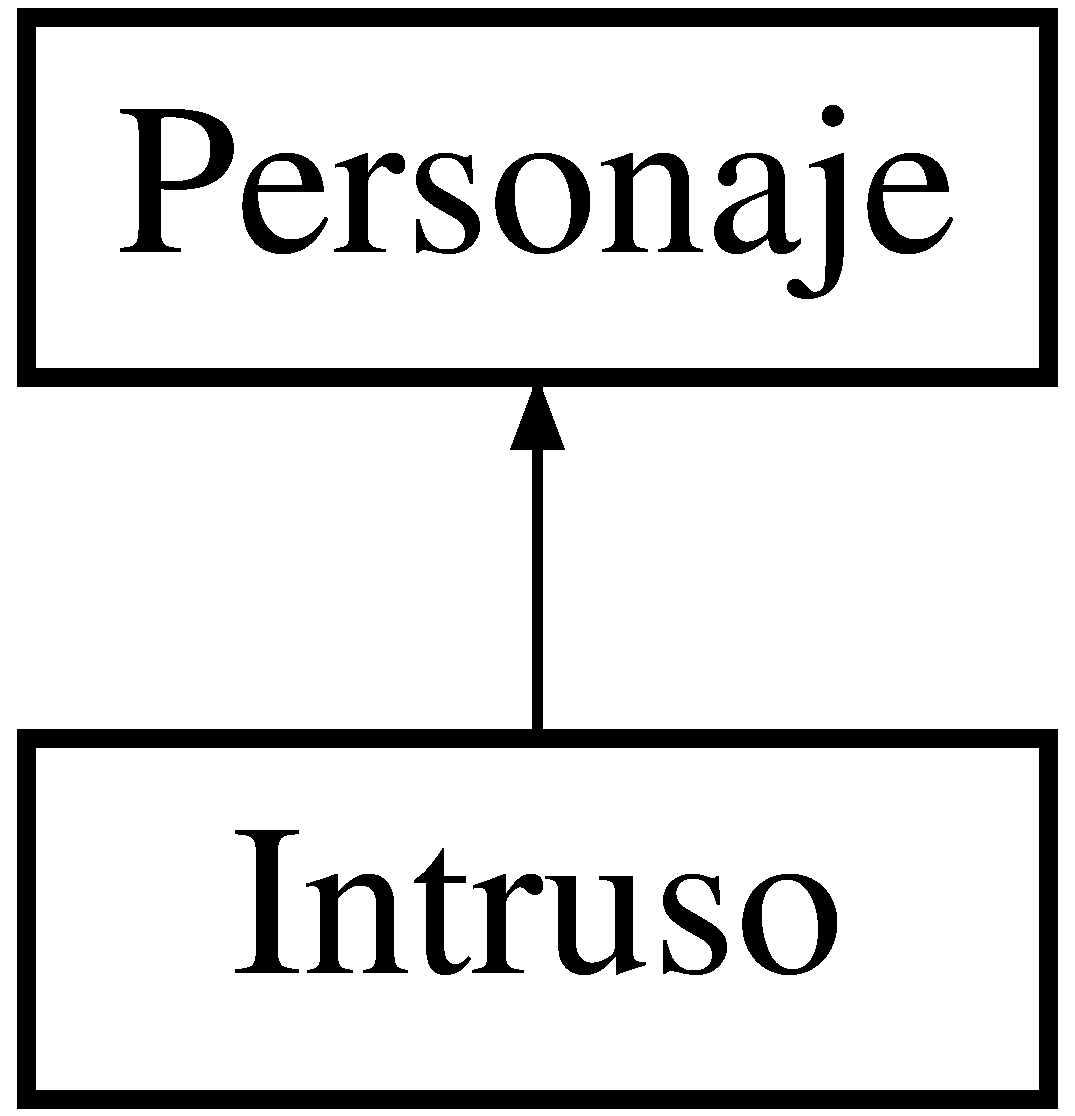
\includegraphics[height=2cm]{classIntruso}
\end{center}
\end{figure}
\subsection*{Public Member Functions}
\begin{CompactItemize}
\item 
\hyperlink{classIntruso_f36bc9ec8ef7b46e9335c6842908a527}{Intruso} ()
\item 
\hyperlink{classIntruso_c8f76c5d9e67549e75cb816820867e7f}{Intruso} (char m, string n, int t, int ids, int idp)
\item 
void \hyperlink{classIntruso_06a5d236e669e5add8b1c6472303133e}{mostrar} ()
\item 
void \hyperlink{classIntruso_979c89c596d92d8ce69b8af5e556d62d}{escribeLog} (ofstream \&f)
\item 
void \hyperlink{classIntruso_6d239cda2dc32af27e50ba84524e4179}{caminoMinimo} (int origen, int destino, \hyperlink{classplanta}{planta} $\ast$pl)
\item 
void \hyperlink{classIntruso_2898ae82386e99d361f6f131122b7be1}{ruta} (ofstream \&f)
\item 
void \hyperlink{classIntruso_0f0142b1852ed9f0431af335d3ff6f14}{escribeLogRuta} (ofstream \&f)
\item 
void \hyperlink{classIntruso_dee71b00225e294086d8980625a32ab3}{accionUno} ()
\item 
void \hyperlink{classIntruso_6fef0ae823fdabc05796413f53d073e5}{accionDos} ()
\item 
void \hyperlink{classIntruso_52e521cc66983d5a9f20f3424818e6e4}{accionTres} ()
\item 
void \hyperlink{classIntruso_99e215b1df4387b629f25349378d3bbb}{accionCuatro} ()
\item 
\hyperlink{classIntruso_947673866dbb60c76b40eff5ab139bcd}{$\sim$Intruso} ()
\end{CompactItemize}


\subsection{Detailed Description}
\begin{Desc}
\item[Author:]Carlos,,, $<$carlos-linux$>$ \end{Desc}


\subsection{Constructor \& Destructor Documentation}
\hypertarget{classIntruso_f36bc9ec8ef7b46e9335c6842908a527}{
\index{Intruso@{Intruso}!Intruso@{Intruso}}
\index{Intruso@{Intruso}!Intruso@{Intruso}}
\subsubsection[Intruso]{\setlength{\rightskip}{0pt plus 5cm}Intruso::Intruso ()}}
\label{classIntruso_f36bc9ec8ef7b46e9335c6842908a527}


Constructor por defecto de mi clase intruso \begin{Desc}
\item[Parameters:]
\begin{description}
\item[{\em \char`\"{}\char`\"{}}]no recibe parametros \end{description}
\end{Desc}
\begin{Desc}
\item[Returns:]No retorna ningun valor \end{Desc}
\hypertarget{classIntruso_c8f76c5d9e67549e75cb816820867e7f}{
\index{Intruso@{Intruso}!Intruso@{Intruso}}
\index{Intruso@{Intruso}!Intruso@{Intruso}}
\subsubsection[Intruso]{\setlength{\rightskip}{0pt plus 5cm}Intruso::Intruso (char {\em m}, \/  string {\em n}, \/  int {\em t}, \/  int {\em ids}, \/  int {\em idp})}}
\label{classIntruso_c8f76c5d9e67549e75cb816820867e7f}


Constructor parametrizado de mi clase intruso \begin{Desc}
\item[Parameters:]
\begin{description}
\item[{\em m}]es la marca de mi personaje de tipo intruso \item[{\em n}]es la cadena asociada al nombre de mi personaje de tipo intruso \item[{\em t}]es un entero asociado al turno del personaje del tipo intruso \item[{\em ids}]es un entero asociado al identificador de la \hyperlink{classsala}{sala} de mi personaje del tipo intruso \item[{\em idp}]es un entero asociado al identificador de la \hyperlink{classplanta}{planta} de mi personaje del tipo intruso \end{description}
\end{Desc}
\begin{Desc}
\item[Returns:]No retorna ningun valor \end{Desc}
\hypertarget{classIntruso_947673866dbb60c76b40eff5ab139bcd}{
\index{Intruso@{Intruso}!$\sim$Intruso@{$\sim$Intruso}}
\index{$\sim$Intruso@{$\sim$Intruso}!Intruso@{Intruso}}
\subsubsection[$\sim$Intruso]{\setlength{\rightskip}{0pt plus 5cm}Intruso::$\sim$Intruso ()}}
\label{classIntruso_947673866dbb60c76b40eff5ab139bcd}


Destructor de mi clase intruso \begin{Desc}
\item[Parameters:]
\begin{description}
\item[{\em \char`\"{}\char`\"{}}]no recibe parametros \end{description}
\end{Desc}
\begin{Desc}
\item[Returns:]No retorna ningun valor \end{Desc}


\subsection{Member Function Documentation}
\hypertarget{classIntruso_06a5d236e669e5add8b1c6472303133e}{
\index{Intruso@{Intruso}!mostrar@{mostrar}}
\index{mostrar@{mostrar}!Intruso@{Intruso}}
\subsubsection[mostrar]{\setlength{\rightskip}{0pt plus 5cm}void Intruso::mostrar ()\hspace{0.3cm}{\tt  \mbox{[}virtual\mbox{]}}}}
\label{classIntruso_06a5d236e669e5add8b1c6472303133e}


Metodo mostrar (por pantalla) de mi clase intruso \begin{Desc}
\item[Parameters:]
\begin{description}
\item[{\em \char`\"{}\char`\"{}}]no recibe parametros \end{description}
\end{Desc}
\begin{Desc}
\item[Returns:]No retorna ningun valor \end{Desc}


Reimplemented from \hyperlink{classPersonaje_e9f6bd8027b8a5c2e660a327d9e513ca}{Personaje}.\hypertarget{classIntruso_979c89c596d92d8ce69b8af5e556d62d}{
\index{Intruso@{Intruso}!escribeLog@{escribeLog}}
\index{escribeLog@{escribeLog}!Intruso@{Intruso}}
\subsubsection[escribeLog]{\setlength{\rightskip}{0pt plus 5cm}void Intruso::escribeLog (ofstream \& {\em f})\hspace{0.3cm}{\tt  \mbox{[}virtual\mbox{]}}}}
\label{classIntruso_979c89c596d92d8ce69b8af5e556d62d}


Metodo que escribe la informacion correspondiente al intruso en mi registro.log \begin{Desc}
\item[Parameters:]
\begin{description}
\item[{\em f}]es un flujo de entrada salida que escribe en mi fichero la informacion correspondiente al personaje de tipo intruso \end{description}
\end{Desc}
\begin{Desc}
\item[Returns:]No retorna ningun valor \end{Desc}


Reimplemented from \hyperlink{classPersonaje_86fe4a1ff708072d98c6be42bbd512ea}{Personaje}.\hypertarget{classIntruso_6d239cda2dc32af27e50ba84524e4179}{
\index{Intruso@{Intruso}!caminoMinimo@{caminoMinimo}}
\index{caminoMinimo@{caminoMinimo}!Intruso@{Intruso}}
\subsubsection[caminoMinimo]{\setlength{\rightskip}{0pt plus 5cm}void Intruso::caminoMinimo (int {\em origen}, \/  int {\em destino}, \/  {\bf planta} $\ast$ {\em pl})}}
\label{classIntruso_6d239cda2dc32af27e50ba84524e4179}


Metodo calcula el camino minimo entre 2 nodos de la \hyperlink{classplanta}{planta} que recibe como parametro (pl en este caso) \begin{Desc}
\item[Parameters:]
\begin{description}
\item[{\em origen}]es un entero que se corresponde con el origen del grafo donde empieza mi camino \item[{\em destino}]es un entero que se corresponde con el destino del grafo donde termina mi camino \item[{\em pl}]es un puntero a un objeto de la clase Planta \end{description}
\end{Desc}
\begin{Desc}
\item[Returns:]No retorna ningun valor \end{Desc}
\hypertarget{classIntruso_2898ae82386e99d361f6f131122b7be1}{
\index{Intruso@{Intruso}!ruta@{ruta}}
\index{ruta@{ruta}!Intruso@{Intruso}}
\subsubsection[ruta]{\setlength{\rightskip}{0pt plus 5cm}void Intruso::ruta (ofstream \& {\em f})\hspace{0.3cm}{\tt  \mbox{[}virtual\mbox{]}}}}
\label{classIntruso_2898ae82386e99d361f6f131122b7be1}


Metodo que calcula la ruta del personaje de tipo intruso y escribe en el registro.log su ruta correspondiente \begin{Desc}
\item[Parameters:]
\begin{description}
\item[{\em f}]es un flujo de entrada salida \end{description}
\end{Desc}
\begin{Desc}
\item[Returns:]No retorna ningun valor \end{Desc}


Reimplemented from \hyperlink{classPersonaje_f6dc20013805229005dfb87fc6f273b5}{Personaje}.\hypertarget{classIntruso_0f0142b1852ed9f0431af335d3ff6f14}{
\index{Intruso@{Intruso}!escribeLogRuta@{escribeLogRuta}}
\index{escribeLogRuta@{escribeLogRuta}!Intruso@{Intruso}}
\subsubsection[escribeLogRuta]{\setlength{\rightskip}{0pt plus 5cm}void Intruso::escribeLogRuta (ofstream \& {\em f})}}
\label{classIntruso_0f0142b1852ed9f0431af335d3ff6f14}


Metodo que escribe en mi registro.log la informacion correspondiente al personaje de tipo intruso \begin{Desc}
\item[Parameters:]
\begin{description}
\item[{\em f}]es un flujo de entrada salida \end{description}
\end{Desc}
\begin{Desc}
\item[Returns:]No retorna ningun valor \end{Desc}
\hypertarget{classIntruso_dee71b00225e294086d8980625a32ab3}{
\index{Intruso@{Intruso}!accionUno@{accionUno}}
\index{accionUno@{accionUno}!Intruso@{Intruso}}
\subsubsection[accionUno]{\setlength{\rightskip}{0pt plus 5cm}void Intruso::accionUno ()\hspace{0.3cm}{\tt  \mbox{[}virtual\mbox{]}}}}
\label{classIntruso_dee71b00225e294086d8980625a32ab3}


Metodo que realiza la accion uno del intruso \begin{Desc}
\item[Parameters:]
\begin{description}
\item[{\em \char`\"{}\char`\"{}}]no recibe parametros \end{description}
\end{Desc}
\begin{Desc}
\item[Returns:]No retorna ningun valor \end{Desc}


Reimplemented from \hyperlink{classPersonaje_0454b75ccc8f7e33f03e2cfb2c59e725}{Personaje}.\hypertarget{classIntruso_6fef0ae823fdabc05796413f53d073e5}{
\index{Intruso@{Intruso}!accionDos@{accionDos}}
\index{accionDos@{accionDos}!Intruso@{Intruso}}
\subsubsection[accionDos]{\setlength{\rightskip}{0pt plus 5cm}void Intruso::accionDos ()\hspace{0.3cm}{\tt  \mbox{[}virtual\mbox{]}}}}
\label{classIntruso_6fef0ae823fdabc05796413f53d073e5}


Metodo que realiza la accion dos del intruso \begin{Desc}
\item[Parameters:]
\begin{description}
\item[{\em \char`\"{}\char`\"{}}]no recibe parametros \end{description}
\end{Desc}
\begin{Desc}
\item[Returns:]No retorna ningun valor \end{Desc}


Reimplemented from \hyperlink{classPersonaje_af7763eb6099390038b7833129a1ef9f}{Personaje}.\hypertarget{classIntruso_52e521cc66983d5a9f20f3424818e6e4}{
\index{Intruso@{Intruso}!accionTres@{accionTres}}
\index{accionTres@{accionTres}!Intruso@{Intruso}}
\subsubsection[accionTres]{\setlength{\rightskip}{0pt plus 5cm}void Intruso::accionTres ()\hspace{0.3cm}{\tt  \mbox{[}virtual\mbox{]}}}}
\label{classIntruso_52e521cc66983d5a9f20f3424818e6e4}


Metodo que realiza la accion tres del intruso \begin{Desc}
\item[Parameters:]
\begin{description}
\item[{\em \char`\"{}\char`\"{}}]no recibe parametros \end{description}
\end{Desc}
\begin{Desc}
\item[Returns:]No retorna ningun valor \end{Desc}


Reimplemented from \hyperlink{classPersonaje_85c25ff0362bf4f4f5e69965c1ae4cfb}{Personaje}.\hypertarget{classIntruso_99e215b1df4387b629f25349378d3bbb}{
\index{Intruso@{Intruso}!accionCuatro@{accionCuatro}}
\index{accionCuatro@{accionCuatro}!Intruso@{Intruso}}
\subsubsection[accionCuatro]{\setlength{\rightskip}{0pt plus 5cm}void Intruso::accionCuatro ()\hspace{0.3cm}{\tt  \mbox{[}virtual\mbox{]}}}}
\label{classIntruso_99e215b1df4387b629f25349378d3bbb}


Metodo que realiza la accion cuatro del intruso \begin{Desc}
\item[Parameters:]
\begin{description}
\item[{\em \char`\"{}\char`\"{}}]no recibe parametros \end{description}
\end{Desc}
\begin{Desc}
\item[Returns:]No retorna ningun valor \end{Desc}


Reimplemented from \hyperlink{classPersonaje_3aed5959a6a829819e0b0a6dcca9c2e4}{Personaje}.

The documentation for this class was generated from the following files:\begin{CompactItemize}
\item 
Desktop/academia\_\-lp2/EC3\_\-LPII/src/intruso.h\item 
Desktop/academia\_\-lp2/EC3\_\-LPII/src/intruso.cpp\end{CompactItemize}

\hypertarget{classLider}{
\section{Lider Class Reference}
\label{classLider}\index{Lider@{Lider}}
}
{\tt \#include $<$lider.h$>$}

Inheritance diagram for Lider::\begin{figure}[H]
\begin{center}
\leavevmode
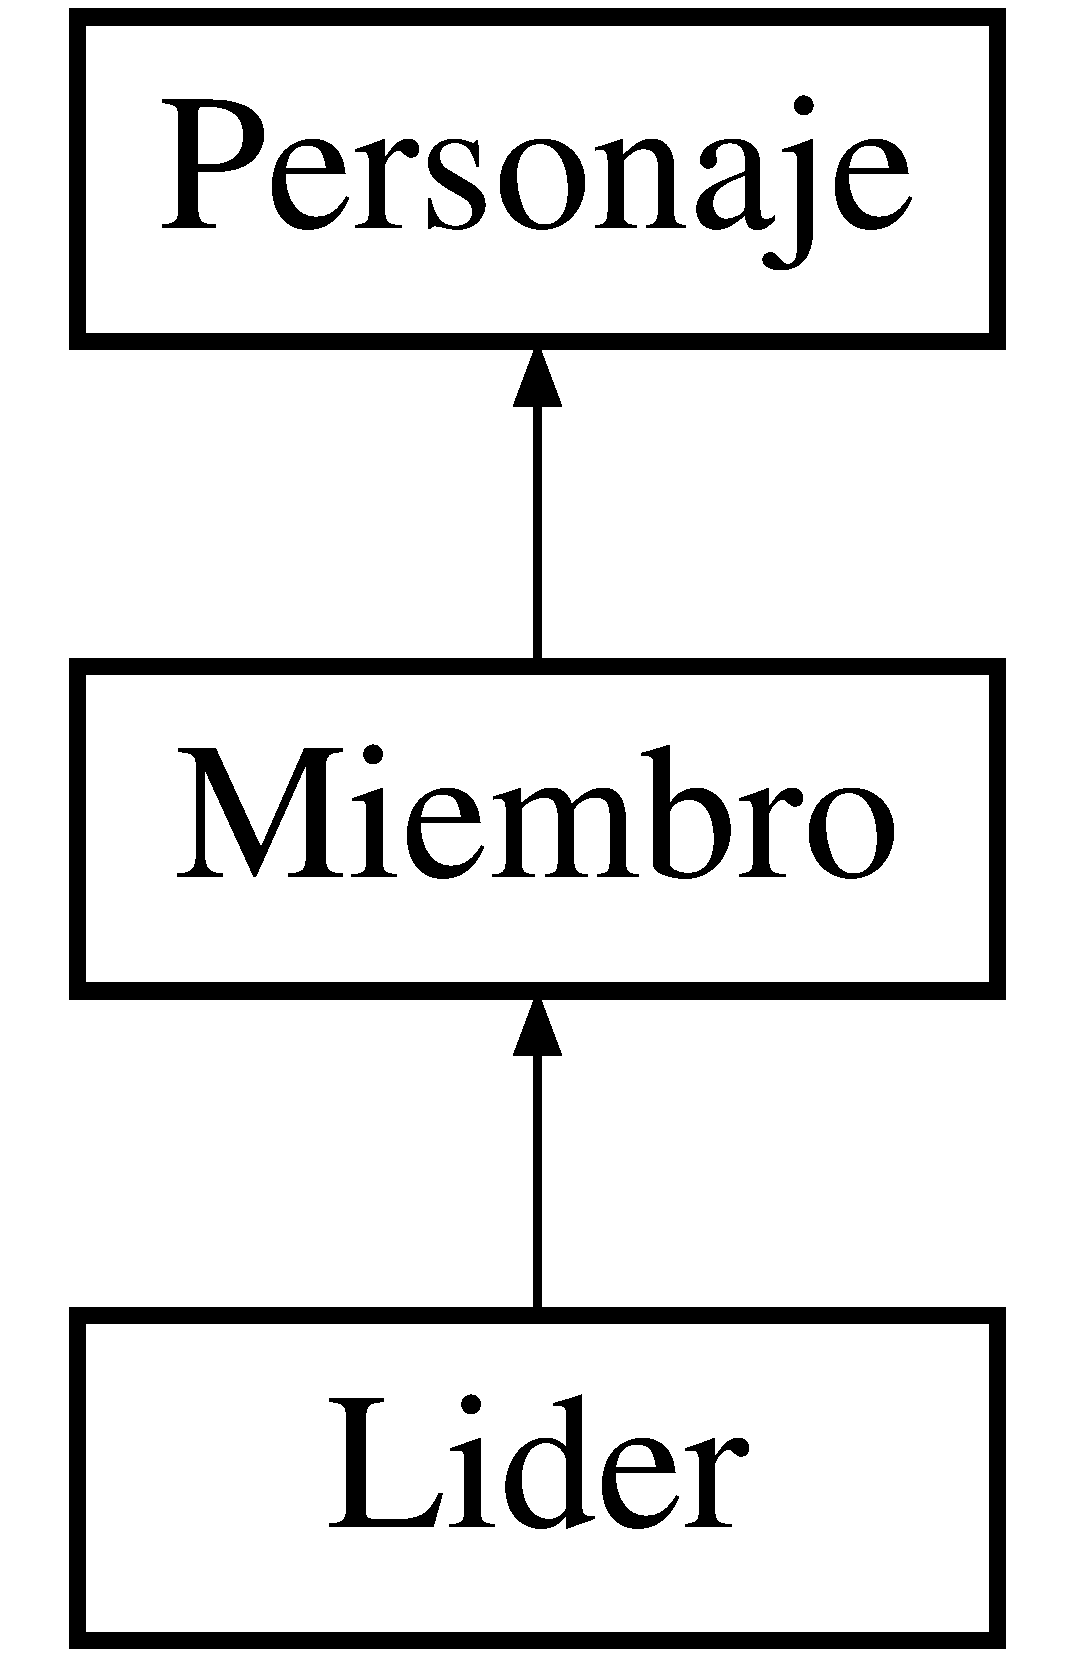
\includegraphics[height=3cm]{classLider}
\end{center}
\end{figure}
\subsection*{Public Member Functions}
\begin{CompactItemize}
\item 
\hyperlink{classLider_bbdd9719261866f4f316620b4319d7e6}{Lider} ()
\item 
\hyperlink{classLider_16da42712d18eb29d78b81613f3d916d}{Lider} (char m, string n, int t, int ids, int idp, string sec, char mov)
\item 
void \hyperlink{classLider_8b7b93efc0b6cecbab4ae82992ebcd11}{setMovimiento} (char m)
\item 
char \hyperlink{classLider_2fb77f30c5ebb7bce39dc7ee4711d4d2}{getMovimiento} ()
\item 
void \hyperlink{classLider_84acf3920a695ab792f9bbcb494ea7c8}{setSecuenciaOrientaciones} (string s)
\item 
void \hyperlink{classLider_38d5268d1d780494277063ce96c52881}{getSecuenciaOrientaciones} (string \&s)
\item 
void \hyperlink{classLider_125acbb3a1432f217efdc9826a2b8d8f}{mostrar} ()
\item 
void \hyperlink{classLider_fcd179370f87dbc08bf6619ff9742f66}{escribeLog} (ofstream \&f)
\item 
void \hyperlink{classLider_6b98929df0d59cd29b85e6fb8aeb36f1}{ruta} (ofstream \&f)
\item 
void \hyperlink{classLider_87a0b4fca538efa5c9b7d01992f362e6}{actualizarMovimiento} ()
\item 
bool \hyperlink{classLider_9b40d8d989e80fbfd39a17bac209b73e}{recorrerVecinos} (int ids, stack$<$ char $>$ \&secorientaciones, stack$<$ int $>$ \&idvecinos, set$<$ int $>$ \&vecinos)
\item 
void \hyperlink{classLider_4643215eb946b9bd002d6882c5a24aeb}{escribeLogRuta} (ofstream \&f, stack$<$ char $>$ \&s, stack$<$ int $>$ \&idsalas)
\item 
void \hyperlink{classLider_2729cb612e6ca2d2750f48b85743107e}{accionUno} ()
\item 
void \hyperlink{classLider_51fb2d9c6dfe283a13d61b8f546068f3}{accionDos} ()
\item 
void \hyperlink{classLider_993a29f5a5615bd8a41dfe550dfccb61}{accionTres} ()
\item 
\hyperlink{classLider_64481cdebf71c9b28ec7aef689fed43e}{$\sim$Lider} ()
\end{CompactItemize}


\subsection{Detailed Description}
\begin{Desc}
\item[Author:]Carlos,,, $<$carlos-linux$>$ \end{Desc}


\subsection{Constructor \& Destructor Documentation}
\hypertarget{classLider_bbdd9719261866f4f316620b4319d7e6}{
\index{Lider@{Lider}!Lider@{Lider}}
\index{Lider@{Lider}!Lider@{Lider}}
\subsubsection[Lider]{\setlength{\rightskip}{0pt plus 5cm}Lider::Lider ()}}
\label{classLider_bbdd9719261866f4f316620b4319d7e6}


Constructor por defecto de mi clase lider \begin{Desc}
\item[Parameters:]
\begin{description}
\item[{\em \char`\"{}\char`\"{}}]no recibe parametros \end{description}
\end{Desc}
\begin{Desc}
\item[Returns:]No retorna ningun valor \end{Desc}
\hypertarget{classLider_16da42712d18eb29d78b81613f3d916d}{
\index{Lider@{Lider}!Lider@{Lider}}
\index{Lider@{Lider}!Lider@{Lider}}
\subsubsection[Lider]{\setlength{\rightskip}{0pt plus 5cm}Lider::Lider (char {\em m}, \/  string {\em n}, \/  int {\em t}, \/  int {\em ids}, \/  int {\em idp}, \/  string {\em sec}, \/  char {\em mov})}}
\label{classLider_16da42712d18eb29d78b81613f3d916d}


Constructor parametrizado de mi clase lider \begin{Desc}
\item[Parameters:]
\begin{description}
\item[{\em m}]es un caracter correspondiente a la marca de mi personaje de tipo lider \item[{\em n}]es una cadena correspondiente al nombre de mi personaje del tipo lider \item[{\em t}]es un entero correspondiente al turno de mi personaje del tipo lider \item[{\em ids}]es un entero correspondiente al identificador de la \hyperlink{classsala}{sala} de mi personaje del tipo lider \item[{\em idp}]es un entero correspondiente al identificador de la \hyperlink{classplanta}{planta} de mi personaje del tipo lider \item[{\em sec}]es una cadena que se corresponde con la secuencia de orientaciones que sigue mi personaje del tipo lider \item[{\em mov}]es un caracter que se corresponde con el movimiento asociado a mi personaje del tipo lider \end{description}
\end{Desc}
\begin{Desc}
\item[Returns:]No retorna ningun valor \end{Desc}
\hypertarget{classLider_64481cdebf71c9b28ec7aef689fed43e}{
\index{Lider@{Lider}!$\sim$Lider@{$\sim$Lider}}
\index{$\sim$Lider@{$\sim$Lider}!Lider@{Lider}}
\subsubsection[$\sim$Lider]{\setlength{\rightskip}{0pt plus 5cm}Lider::$\sim$Lider ()}}
\label{classLider_64481cdebf71c9b28ec7aef689fed43e}


Destructor de mi clase lider \begin{Desc}
\item[Parameters:]
\begin{description}
\item[{\em \char`\"{}\char`\"{}}]no recibe parametros \end{description}
\end{Desc}
\begin{Desc}
\item[Returns:]No retorna ningun valor \end{Desc}


\subsection{Member Function Documentation}
\hypertarget{classLider_8b7b93efc0b6cecbab4ae82992ebcd11}{
\index{Lider@{Lider}!setMovimiento@{setMovimiento}}
\index{setMovimiento@{setMovimiento}!Lider@{Lider}}
\subsubsection[setMovimiento]{\setlength{\rightskip}{0pt plus 5cm}void Lider::setMovimiento (char {\em m})}}
\label{classLider_8b7b93efc0b6cecbab4ae82992ebcd11}


Metodo que establece a mi atributo movimiento el valor de m \begin{Desc}
\item[Parameters:]
\begin{description}
\item[{\em m}]es un parametro de entrada del tipo caracter que establece el movimiento de mi personaje de tipo lider \end{description}
\end{Desc}
\begin{Desc}
\item[Returns:]No retorna ningun valor \end{Desc}
\hypertarget{classLider_2fb77f30c5ebb7bce39dc7ee4711d4d2}{
\index{Lider@{Lider}!getMovimiento@{getMovimiento}}
\index{getMovimiento@{getMovimiento}!Lider@{Lider}}
\subsubsection[getMovimiento]{\setlength{\rightskip}{0pt plus 5cm}char Lider::getMovimiento ()}}
\label{classLider_2fb77f30c5ebb7bce39dc7ee4711d4d2}


Metodo que devuelve el caracter correspondiente al movimiento de mi personaje de tipo lider \begin{Desc}
\item[Parameters:]
\begin{description}
\item[{\em \char`\"{}\char`\"{}}]no recibe parametros \end{description}
\end{Desc}
\begin{Desc}
\item[Returns:]Retorna un caracter que se corresponde con el movimiento asociado a mi personaje de tipo lider \end{Desc}
\hypertarget{classLider_84acf3920a695ab792f9bbcb494ea7c8}{
\index{Lider@{Lider}!setSecuenciaOrientaciones@{setSecuenciaOrientaciones}}
\index{setSecuenciaOrientaciones@{setSecuenciaOrientaciones}!Lider@{Lider}}
\subsubsection[setSecuenciaOrientaciones]{\setlength{\rightskip}{0pt plus 5cm}void Lider::setSecuenciaOrientaciones (string {\em s})}}
\label{classLider_84acf3920a695ab792f9bbcb494ea7c8}


Metodo que asigna a mi atributo secuenciaorientaciones la cadena s \begin{Desc}
\item[Parameters:]
\begin{description}
\item[{\em s}]es un parametro de entrada del tipo string \end{description}
\end{Desc}
\begin{Desc}
\item[Returns:]No retorna ningun valor \end{Desc}
\hypertarget{classLider_38d5268d1d780494277063ce96c52881}{
\index{Lider@{Lider}!getSecuenciaOrientaciones@{getSecuenciaOrientaciones}}
\index{getSecuenciaOrientaciones@{getSecuenciaOrientaciones}!Lider@{Lider}}
\subsubsection[getSecuenciaOrientaciones]{\setlength{\rightskip}{0pt plus 5cm}void Lider::getSecuenciaOrientaciones (string \& {\em s})}}
\label{classLider_38d5268d1d780494277063ce96c52881}


Metodo que devuelve en s la cadena correspondiente a mi atributo secuenciaorientaciones \begin{Desc}
\item[Parameters:]
\begin{description}
\item[{\em s}]es un parametro de entrada salida que almacena la cadena secuenciaorientaciones \end{description}
\end{Desc}
\begin{Desc}
\item[Returns:]No retorna ningun valor \end{Desc}
\hypertarget{classLider_125acbb3a1432f217efdc9826a2b8d8f}{
\index{Lider@{Lider}!mostrar@{mostrar}}
\index{mostrar@{mostrar}!Lider@{Lider}}
\subsubsection[mostrar]{\setlength{\rightskip}{0pt plus 5cm}void Lider::mostrar ()\hspace{0.3cm}{\tt  \mbox{[}virtual\mbox{]}}}}
\label{classLider_125acbb3a1432f217efdc9826a2b8d8f}


Metodo que muestra por pantalla el tipo de personaje que se trata, en este caso , es un lider \begin{Desc}
\item[Parameters:]
\begin{description}
\item[{\em \char`\"{}\char`\"{}}]no recibe parametros \end{description}
\end{Desc}
\begin{Desc}
\item[Returns:]No retorna ningun valor \end{Desc}


Reimplemented from \hyperlink{classMiembro_28498c7229e81e64d0cb7ea69515dca0}{Miembro}.\hypertarget{classLider_fcd179370f87dbc08bf6619ff9742f66}{
\index{Lider@{Lider}!escribeLog@{escribeLog}}
\index{escribeLog@{escribeLog}!Lider@{Lider}}
\subsubsection[escribeLog]{\setlength{\rightskip}{0pt plus 5cm}void Lider::escribeLog (ofstream \& {\em f})\hspace{0.3cm}{\tt  \mbox{[}virtual\mbox{]}}}}
\label{classLider_fcd179370f87dbc08bf6619ff9742f66}


Metodo que escribe en mi registro.log la informacion de mi personaje de tipo lider y además escribo la informacion correspondiente a los personajes que se encuentran en el atributo grupo \begin{Desc}
\item[Parameters:]
\begin{description}
\item[{\em f}]es un flujo de entrada salida \end{description}
\end{Desc}
\begin{Desc}
\item[Returns:]No retorna ningun valor \end{Desc}


aqui hago el log de cada miembro que hay en su grupo 

Reimplemented from \hyperlink{classPersonaje_86fe4a1ff708072d98c6be42bbd512ea}{Personaje}.\hypertarget{classLider_6b98929df0d59cd29b85e6fb8aeb36f1}{
\index{Lider@{Lider}!ruta@{ruta}}
\index{ruta@{ruta}!Lider@{Lider}}
\subsubsection[ruta]{\setlength{\rightskip}{0pt plus 5cm}void Lider::ruta (ofstream \& {\em f})\hspace{0.3cm}{\tt  \mbox{[}virtual\mbox{]}}}}
\label{classLider_6b98929df0d59cd29b85e6fb8aeb36f1}


Metodo que calcula la ruta de mi personaje de tipo lider \begin{Desc}
\item[Parameters:]
\begin{description}
\item[{\em f}]es un flujo de entrada salida \end{description}
\end{Desc}
\begin{Desc}
\item[Returns:]No retorna ningun valor \end{Desc}


Reimplemented from \hyperlink{classPersonaje_f6dc20013805229005dfb87fc6f273b5}{Personaje}.\hypertarget{classLider_87a0b4fca538efa5c9b7d01992f362e6}{
\index{Lider@{Lider}!actualizarMovimiento@{actualizarMovimiento}}
\index{actualizarMovimiento@{actualizarMovimiento}!Lider@{Lider}}
\subsubsection[actualizarMovimiento]{\setlength{\rightskip}{0pt plus 5cm}void Lider::actualizarMovimiento ()}}
\label{classLider_87a0b4fca538efa5c9b7d01992f362e6}


Metodo actualiza el movimiento de mi personaje de tipo lider \begin{Desc}
\item[Parameters:]
\begin{description}
\item[{\em \char`\"{}\char`\"{}}]no recibe parametros \end{description}
\end{Desc}
\begin{Desc}
\item[Returns:]No retorna ningun valor \end{Desc}
\hypertarget{classLider_9b40d8d989e80fbfd39a17bac209b73e}{
\index{Lider@{Lider}!recorrerVecinos@{recorrerVecinos}}
\index{recorrerVecinos@{recorrerVecinos}!Lider@{Lider}}
\subsubsection[recorrerVecinos]{\setlength{\rightskip}{0pt plus 5cm}bool Lider::recorrerVecinos (int {\em ids}, \/  stack$<$ char $>$ \& {\em secorientaciones}, \/  stack$<$ int $>$ \& {\em idsalas}, \/  set$<$ int $>$ \& {\em vecinos})}}
\label{classLider_9b40d8d989e80fbfd39a17bac209b73e}


Metodo booleano que calcula los vecinos de mi personaje de tipo lider \begin{Desc}
\item[Parameters:]
\begin{description}
\item[{\em ids}]es un parametro de entrada del tipo entero correspondiente al identificador de la \hyperlink{classsala}{sala} \item[{\em secorientaciones}]es un parametro de entrada salida del tipo stack (pila) que almacena los caracteres correspondiente a la posicion cardinal de los vecinos que se van obteniendo \item[{\em idsalas}]es un parametro de entrada salida del tipo stack(pila) que almacena los enteros correspondientes a los identificadores de las salas de los vecinos donde se mueve mi personaje de tipo lider \item[{\em vecinos}]es un parametro de entrada salida del tipo set (conjunto) de enteros que almacena los enteros correspondientes a los identificadores de las salas de los vecinos de mi personaje de tipo lider\end{description}
\end{Desc}
\begin{Desc}
\item[Returns:]Retorna true si el personaje del tipo lider alcanza la \hyperlink{classsala}{sala} de salida de la \hyperlink{classplanta}{planta} y false en caso contrario \end{Desc}
\hypertarget{classLider_4643215eb946b9bd002d6882c5a24aeb}{
\index{Lider@{Lider}!escribeLogRuta@{escribeLogRuta}}
\index{escribeLogRuta@{escribeLogRuta}!Lider@{Lider}}
\subsubsection[escribeLogRuta]{\setlength{\rightskip}{0pt plus 5cm}void Lider::escribeLogRuta (ofstream \& {\em f}, \/  stack$<$ char $>$ \& {\em sec}, \/  stack$<$ int $>$ \& {\em idsalas})}}
\label{classLider_4643215eb946b9bd002d6882c5a24aeb}


Metodo que escribe en mi registro.log toda la informacion correspondiente a la ruta de mi personaje del tipo lider \begin{Desc}
\item[Parameters:]
\begin{description}
\item[{\em f}]es un flujo de entrada salida \item[{\em sec}]es un parametro de entrada salida del tipo stack(pila) de caracteres que almacena las posiciones cardinales del movimiento de mi personaje del tipo lider \item[{\em idsalas}]es un parametro de entrada salida del tipo stack (pila) que almacena los enteros correspondientes a los identificadores de las salas donde se mueve mi personaje del tipo lider \end{description}
\end{Desc}
\begin{Desc}
\item[Returns:]No retorna ningun valor \end{Desc}
\hypertarget{classLider_2729cb612e6ca2d2750f48b85743107e}{
\index{Lider@{Lider}!accionUno@{accionUno}}
\index{accionUno@{accionUno}!Lider@{Lider}}
\subsubsection[accionUno]{\setlength{\rightskip}{0pt plus 5cm}void Lider::accionUno ()\hspace{0.3cm}{\tt  \mbox{[}virtual\mbox{]}}}}
\label{classLider_2729cb612e6ca2d2750f48b85743107e}


Metodo que realiza la accion uno del lider \begin{Desc}
\item[Parameters:]
\begin{description}
\item[{\em \char`\"{}\char`\"{}}]no recibe parametros \end{description}
\end{Desc}
\begin{Desc}
\item[Returns:]No retorna ningun valor \end{Desc}


aqui pruebo con cada una de las llaves que llevan los miembros en el grupo (sólo con la 1ª de cada uno) 

Reimplemented from \hyperlink{classPersonaje_0454b75ccc8f7e33f03e2cfb2c59e725}{Personaje}.\hypertarget{classLider_51fb2d9c6dfe283a13d61b8f546068f3}{
\index{Lider@{Lider}!accionDos@{accionDos}}
\index{accionDos@{accionDos}!Lider@{Lider}}
\subsubsection[accionDos]{\setlength{\rightskip}{0pt plus 5cm}void Lider::accionDos ()\hspace{0.3cm}{\tt  \mbox{[}virtual\mbox{]}}}}
\label{classLider_51fb2d9c6dfe283a13d61b8f546068f3}


Metodo realiza la accion dos del lider \begin{Desc}
\item[Parameters:]
\begin{description}
\item[{\em \char`\"{}\char`\"{}}]no recibe parametros \end{description}
\end{Desc}
\begin{Desc}
\item[Returns:]No retorna ningun valor \end{Desc}


Si estoy en la \hyperlink{classsala}{sala} de salida y la \hyperlink{classpuerta}{puerta} está cerrada NO me puedo mover 

Reimplemented from \hyperlink{classPersonaje_af7763eb6099390038b7833129a1ef9f}{Personaje}.\hypertarget{classLider_993a29f5a5615bd8a41dfe550dfccb61}{
\index{Lider@{Lider}!accionTres@{accionTres}}
\index{accionTres@{accionTres}!Lider@{Lider}}
\subsubsection[accionTres]{\setlength{\rightskip}{0pt plus 5cm}void Lider::accionTres ()\hspace{0.3cm}{\tt  \mbox{[}virtual\mbox{]}}}}
\label{classLider_993a29f5a5615bd8a41dfe550dfccb61}


Metodo realiza la accion tres del lider \begin{Desc}
\item[Parameters:]
\begin{description}
\item[{\em \char`\"{}\char`\"{}}]no recibe parametros \end{description}
\end{Desc}
\begin{Desc}
\item[Returns:]No retorna ningun valor \end{Desc}


Reimplemented from \hyperlink{classPersonaje_85c25ff0362bf4f4f5e69965c1ae4cfb}{Personaje}.

The documentation for this class was generated from the following files:\begin{CompactItemize}
\item 
Desktop/academia\_\-lp2/EC3\_\-LPII/src/lider.h\item 
Desktop/academia\_\-lp2/EC3\_\-LPII/src/lider.cpp\end{CompactItemize}

\hypertarget{classLlave}{
\section{Llave Class Reference}
\label{classLlave}\index{Llave@{Llave}}
}
{\tt \#include $<$llave.h$>$}

\subsection*{Public Member Functions}
\begin{CompactItemize}
\item 
\hyperlink{classLlave_a2f4f79518899176f8760ce8d0cc6c26}{Llave} ()
\item 
void \hyperlink{classLlave_c80fb30127165c307bc38873545e57fc}{setIdentificador} (int n)
\item 
int \hyperlink{classLlave_21a4a576a987126d469a6eecb167aed1}{getIdentificador} ()
\item 
\hyperlink{classLlave_b3bedc41ed2e5fedbc6d661d625c5cfb}{Llave} (int n)
\item 
int \hyperlink{classLlave_3ed579466201fc80172774d871ece003}{operator==} (\hyperlink{classLlave}{Llave} \&l)
\item 
int \hyperlink{classLlave_932475670e3d7c9e47ca0837d829a7eb}{operator$<$} (\hyperlink{classLlave}{Llave} \&l)
\item 
int \hyperlink{classLlave_be84640478b66d4114fc5995b7981dfb}{operator$>$} (\hyperlink{classLlave}{Llave} \&l)
\item 
int \hyperlink{classLlave_da6d6ec0cb9dc0c04b2b39d4a0dd9128}{operator!=} (\hyperlink{classLlave}{Llave} \&l)
\item 
int \hyperlink{classLlave_82d40399d2418c8e117f62f7df6ee95c}{operator$<$=} (\hyperlink{classLlave}{Llave} \&l)
\item 
int \hyperlink{classLlave_ad93df44517e7d51ceef30182afb8232}{operator$>$=} (\hyperlink{classLlave}{Llave} \&l)
\item 
int \hyperlink{classLlave_635d5c55c24d90520c5460973058b1ef}{operator==} (int n)
\item 
int \hyperlink{classLlave_a6d47e36c8bcd46f7153d00f7ca343d5}{operator$<$} (int n)
\item 
int \hyperlink{classLlave_c5abd96ecfa2d3e8827fce2710b1cbdd}{operator$>$} (int n)
\item 
int \hyperlink{classLlave_c4fdcbca296854f56c8ec7606c15ca40}{operator!=} (int n)
\item 
int \hyperlink{classLlave_6953a596b1bc6e951ef5ca434b5c1036}{operator$<$=} (int n)
\item 
int \hyperlink{classLlave_21d29952725fc8390d668e5ad2094110}{operator$>$=} (int n)
\item 
\hyperlink{classLlave_7db4b83fa86cc3974ac90c6c34c9c56e}{Llave} (const \hyperlink{classLlave}{Llave} \&l)
\item 
\hyperlink{classLlave_b0e13e4c7afa757571506ac3d04e5df2}{$\sim$Llave} ()
\end{CompactItemize}
\subsection*{Friends}
\begin{CompactItemize}
\item 
ostream \& \hyperlink{classLlave_749fde97e089059539e396738c36b7d3}{operator$<$$<$} (ostream \&f, \hyperlink{classLlave}{Llave} \&l)
\end{CompactItemize}


\subsection{Detailed Description}
\begin{Desc}
\item[Author:]Carlos,,, $<$carlos-linux$>$ \end{Desc}


\subsection{Constructor \& Destructor Documentation}
\hypertarget{classLlave_a2f4f79518899176f8760ce8d0cc6c26}{
\index{Llave@{Llave}!Llave@{Llave}}
\index{Llave@{Llave}!Llave@{Llave}}
\subsubsection[Llave]{\setlength{\rightskip}{0pt plus 5cm}Llave::Llave ()}}
\label{classLlave_a2f4f79518899176f8760ce8d0cc6c26}


Constructor por defecto de mi clase \hyperlink{classLlave}{Llave} \begin{Desc}
\item[Parameters:]
\begin{description}
\item[{\em \char`\"{}\char`\"{}}]no recibe parametros \end{description}
\end{Desc}
\begin{Desc}
\item[Returns:]No retorna ningun valor \end{Desc}
\hypertarget{classLlave_b3bedc41ed2e5fedbc6d661d625c5cfb}{
\index{Llave@{Llave}!Llave@{Llave}}
\index{Llave@{Llave}!Llave@{Llave}}
\subsubsection[Llave]{\setlength{\rightskip}{0pt plus 5cm}Llave::Llave (int {\em n})}}
\label{classLlave_b3bedc41ed2e5fedbc6d661d625c5cfb}


Constructor parametrizado de mi clase \hyperlink{classLlave}{Llave} \begin{Desc}
\item[Parameters:]
\begin{description}
\item[{\em n}]es un parametro de entrada del tipo entero \end{description}
\end{Desc}
\begin{Desc}
\item[Returns:]No retorna ningun valor \end{Desc}
\hypertarget{classLlave_7db4b83fa86cc3974ac90c6c34c9c56e}{
\index{Llave@{Llave}!Llave@{Llave}}
\index{Llave@{Llave}!Llave@{Llave}}
\subsubsection[Llave]{\setlength{\rightskip}{0pt plus 5cm}Llave::Llave (const {\bf Llave} \& {\em l})}}
\label{classLlave_7db4b83fa86cc3974ac90c6c34c9c56e}


Constructor por copia de mi clase \hyperlink{classLlave}{Llave} \begin{Desc}
\item[Parameters:]
\begin{description}
\item[{\em l}]es un parametro de entrada salida de la clase \hyperlink{classLlave}{Llave} \end{description}
\end{Desc}
\begin{Desc}
\item[Returns:]No retorna ningun valor \end{Desc}
\hypertarget{classLlave_b0e13e4c7afa757571506ac3d04e5df2}{
\index{Llave@{Llave}!$\sim$Llave@{$\sim$Llave}}
\index{$\sim$Llave@{$\sim$Llave}!Llave@{Llave}}
\subsubsection[$\sim$Llave]{\setlength{\rightskip}{0pt plus 5cm}Llave::$\sim$Llave ()}}
\label{classLlave_b0e13e4c7afa757571506ac3d04e5df2}


Destructor de mi clase Llav e \begin{Desc}
\item[Parameters:]
\begin{description}
\item[{\em \char`\"{}\char`\"{}}]no recibe parametros \end{description}
\end{Desc}
\begin{Desc}
\item[Returns:]No retorna ningun valor \end{Desc}


\subsection{Member Function Documentation}
\hypertarget{classLlave_c80fb30127165c307bc38873545e57fc}{
\index{Llave@{Llave}!setIdentificador@{setIdentificador}}
\index{setIdentificador@{setIdentificador}!Llave@{Llave}}
\subsubsection[setIdentificador]{\setlength{\rightskip}{0pt plus 5cm}void Llave::setIdentificador (int {\em n})}}
\label{classLlave_c80fb30127165c307bc38873545e57fc}


Metodo que establece al atributo identificador de mi clase \hyperlink{classLlave}{Llave} el valor n \begin{Desc}
\item[Parameters:]
\begin{description}
\item[{\em n}]es un parametro de entrada del tipo entero \end{description}
\end{Desc}
\begin{Desc}
\item[Returns:]No retorna ningun valor \end{Desc}
\hypertarget{classLlave_21a4a576a987126d469a6eecb167aed1}{
\index{Llave@{Llave}!getIdentificador@{getIdentificador}}
\index{getIdentificador@{getIdentificador}!Llave@{Llave}}
\subsubsection[getIdentificador]{\setlength{\rightskip}{0pt plus 5cm}int Llave::getIdentificador ()}}
\label{classLlave_21a4a576a987126d469a6eecb167aed1}


Metodo que devuelve el valor entero de mi atributo identificador de mi clase \hyperlink{classLlave}{Llave} \begin{Desc}
\item[Parameters:]
\begin{description}
\item[{\em \char`\"{}\char`\"{}}]no recibe parametros \end{description}
\end{Desc}
\begin{Desc}
\item[Returns:]Retorna el valor entero correspondiente al atributo identificador de mi clase \hyperlink{classLlave}{Llave} \end{Desc}
\hypertarget{classLlave_3ed579466201fc80172774d871ece003}{
\index{Llave@{Llave}!operator==@{operator==}}
\index{operator==@{operator==}!Llave@{Llave}}
\subsubsection[operator==]{\setlength{\rightskip}{0pt plus 5cm}int Llave::operator== ({\bf Llave} \& {\em l})}}
\label{classLlave_3ed579466201fc80172774d871ece003}


Sobrecarga del operador == de mi clase \hyperlink{classLlave}{Llave} \begin{Desc}
\item[Parameters:]
\begin{description}
\item[{\em l}]es un parametro de entrada salida de mi clase \hyperlink{classLlave}{Llave} \end{description}
\end{Desc}
\begin{Desc}
\item[Returns:]No retorna ningun valor \end{Desc}
\hypertarget{classLlave_932475670e3d7c9e47ca0837d829a7eb}{
\index{Llave@{Llave}!operator$<$@{operator$<$}}
\index{operator$<$@{operator$<$}!Llave@{Llave}}
\subsubsection[operator$<$]{\setlength{\rightskip}{0pt plus 5cm}int Llave::operator$<$ ({\bf Llave} \& {\em l})}}
\label{classLlave_932475670e3d7c9e47ca0837d829a7eb}


Sobrecarga del operador \char`\"{}$<$\char`\"{} de mi clase \hyperlink{classLlave}{Llave} \begin{Desc}
\item[Parameters:]
\begin{description}
\item[{\em l}]es un parametro de entrada salida de la clase \hyperlink{classLlave}{Llave} \end{description}
\end{Desc}
\begin{Desc}
\item[Returns:]No retorna ningun valor \end{Desc}
\hypertarget{classLlave_be84640478b66d4114fc5995b7981dfb}{
\index{Llave@{Llave}!operator$>$@{operator$>$}}
\index{operator$>$@{operator$>$}!Llave@{Llave}}
\subsubsection[operator$>$]{\setlength{\rightskip}{0pt plus 5cm}int Llave::operator$>$ ({\bf Llave} \& {\em l})}}
\label{classLlave_be84640478b66d4114fc5995b7981dfb}


sobrecarga del operador \char`\"{}$>$\char`\"{}de mi clase \hyperlink{classLlave}{Llave} \begin{Desc}
\item[Parameters:]
\begin{description}
\item[{\em l}]es un parametro de entrada salida de la clase \hyperlink{classLlave}{Llave} \end{description}
\end{Desc}
\begin{Desc}
\item[Returns:]No retorna ningun valor \end{Desc}
\hypertarget{classLlave_da6d6ec0cb9dc0c04b2b39d4a0dd9128}{
\index{Llave@{Llave}!operator"!=@{operator"!=}}
\index{operator"!=@{operator"!=}!Llave@{Llave}}
\subsubsection[operator"!=]{\setlength{\rightskip}{0pt plus 5cm}int Llave::operator!= ({\bf Llave} \& {\em l})}}
\label{classLlave_da6d6ec0cb9dc0c04b2b39d4a0dd9128}


sobrecarga del operador \char`\"{}!=\char`\"{}de mi clase \hyperlink{classLlave}{Llave} \begin{Desc}
\item[Parameters:]
\begin{description}
\item[{\em l}]es un parametro de entrada salida de la clase \hyperlink{classLlave}{Llave} \end{description}
\end{Desc}
\begin{Desc}
\item[Returns:]No retorna ningun valor \end{Desc}
\hypertarget{classLlave_82d40399d2418c8e117f62f7df6ee95c}{
\index{Llave@{Llave}!operator$<$=@{operator$<$=}}
\index{operator$<$=@{operator$<$=}!Llave@{Llave}}
\subsubsection[operator$<$=]{\setlength{\rightskip}{0pt plus 5cm}int Llave::operator$<$= ({\bf Llave} \& {\em l})}}
\label{classLlave_82d40399d2418c8e117f62f7df6ee95c}


sobrecarga del operador \char`\"{}$<$=\char`\"{}de mi clase \hyperlink{classLlave}{Llave} \begin{Desc}
\item[Parameters:]
\begin{description}
\item[{\em l}]es un parametro de entrada salida de la clase \hyperlink{classLlave}{Llave} \end{description}
\end{Desc}
\begin{Desc}
\item[Returns:]No retorna ningun valor \end{Desc}
\hypertarget{classLlave_ad93df44517e7d51ceef30182afb8232}{
\index{Llave@{Llave}!operator$>$=@{operator$>$=}}
\index{operator$>$=@{operator$>$=}!Llave@{Llave}}
\subsubsection[operator$>$=]{\setlength{\rightskip}{0pt plus 5cm}int Llave::operator$>$= ({\bf Llave} \& {\em l})}}
\label{classLlave_ad93df44517e7d51ceef30182afb8232}


sobrecarga del operador \char`\"{}$>$=\char`\"{}de mi clase \hyperlink{classLlave}{Llave} \begin{Desc}
\item[Parameters:]
\begin{description}
\item[{\em l}]es un parametro de entrada salida de la clase \hyperlink{classLlave}{Llave} \end{description}
\end{Desc}
\begin{Desc}
\item[Returns:]No retorna ningun valor \end{Desc}
\hypertarget{classLlave_635d5c55c24d90520c5460973058b1ef}{
\index{Llave@{Llave}!operator==@{operator==}}
\index{operator==@{operator==}!Llave@{Llave}}
\subsubsection[operator==]{\setlength{\rightskip}{0pt plus 5cm}int Llave::operator== (int {\em n})}}
\label{classLlave_635d5c55c24d90520c5460973058b1ef}


Sobrecarga del operador == para los identificadores de los objetos de la clase \hyperlink{classLlave}{Llave} \begin{Desc}
\item[Parameters:]
\begin{description}
\item[{\em n}]es un parametro de entrada del tipo entero correspondiente al identificador de la llave a comparar \end{description}
\end{Desc}
\begin{Desc}
\item[Returns:]No retorna ningun valor \end{Desc}
\hypertarget{classLlave_a6d47e36c8bcd46f7153d00f7ca343d5}{
\index{Llave@{Llave}!operator$<$@{operator$<$}}
\index{operator$<$@{operator$<$}!Llave@{Llave}}
\subsubsection[operator$<$]{\setlength{\rightskip}{0pt plus 5cm}int Llave::operator$<$ (int {\em n})}}
\label{classLlave_a6d47e36c8bcd46f7153d00f7ca343d5}


sobrecarga del operador \char`\"{}$<$\char`\"{}de mi clase \hyperlink{classLlave}{Llave} \begin{Desc}
\item[Parameters:]
\begin{description}
\item[{\em n}]es un parametro de entrada del tipo entero \end{description}
\end{Desc}
\begin{Desc}
\item[Returns:]No retorna ningun valor \end{Desc}
\hypertarget{classLlave_c5abd96ecfa2d3e8827fce2710b1cbdd}{
\index{Llave@{Llave}!operator$>$@{operator$>$}}
\index{operator$>$@{operator$>$}!Llave@{Llave}}
\subsubsection[operator$>$]{\setlength{\rightskip}{0pt plus 5cm}int Llave::operator$>$ (int {\em n})}}
\label{classLlave_c5abd96ecfa2d3e8827fce2710b1cbdd}


sobrecarga del operador \char`\"{}$>$\char`\"{}de mi clase \hyperlink{classLlave}{Llave} \begin{Desc}
\item[Parameters:]
\begin{description}
\item[{\em n}]es un parametro de entrada del tipo entero \end{description}
\end{Desc}
\begin{Desc}
\item[Returns:]No retorna ningun valor \end{Desc}
\hypertarget{classLlave_c4fdcbca296854f56c8ec7606c15ca40}{
\index{Llave@{Llave}!operator"!=@{operator"!=}}
\index{operator"!=@{operator"!=}!Llave@{Llave}}
\subsubsection[operator"!=]{\setlength{\rightskip}{0pt plus 5cm}int Llave::operator!= (int {\em n})}}
\label{classLlave_c4fdcbca296854f56c8ec7606c15ca40}


sobrecarga del operador \char`\"{}!=\char`\"{}de mi clase \hyperlink{classLlave}{Llave} \begin{Desc}
\item[Parameters:]
\begin{description}
\item[{\em n}]es un parametro de entrada del tipo entero \end{description}
\end{Desc}
\begin{Desc}
\item[Returns:]No retorna ningun valor \end{Desc}
\hypertarget{classLlave_6953a596b1bc6e951ef5ca434b5c1036}{
\index{Llave@{Llave}!operator$<$=@{operator$<$=}}
\index{operator$<$=@{operator$<$=}!Llave@{Llave}}
\subsubsection[operator$<$=]{\setlength{\rightskip}{0pt plus 5cm}int Llave::operator$<$= (int {\em n})}}
\label{classLlave_6953a596b1bc6e951ef5ca434b5c1036}


sobrecarga del operador \char`\"{}$<$=\char`\"{}de mi clase \hyperlink{classLlave}{Llave} \begin{Desc}
\item[Parameters:]
\begin{description}
\item[{\em n}]es un parametro de entrada del tipo entero \end{description}
\end{Desc}
\begin{Desc}
\item[Returns:]No retorna ningun valor \end{Desc}
\hypertarget{classLlave_21d29952725fc8390d668e5ad2094110}{
\index{Llave@{Llave}!operator$>$=@{operator$>$=}}
\index{operator$>$=@{operator$>$=}!Llave@{Llave}}
\subsubsection[operator$>$=]{\setlength{\rightskip}{0pt plus 5cm}int Llave::operator$>$= (int {\em n})}}
\label{classLlave_21d29952725fc8390d668e5ad2094110}


sobrecarga del operador \char`\"{}$>$=\char`\"{}de mi clase \hyperlink{classLlave}{Llave} \begin{Desc}
\item[Parameters:]
\begin{description}
\item[{\em n}]es un parametro de entrada del tipo entero \end{description}
\end{Desc}
\begin{Desc}
\item[Returns:]No retorna ningun valor \end{Desc}


\subsection{Friends And Related Function Documentation}
\hypertarget{classLlave_749fde97e089059539e396738c36b7d3}{
\index{Llave@{Llave}!operator$<$$<$@{operator$<$$<$}}
\index{operator$<$$<$@{operator$<$$<$}!Llave@{Llave}}
\subsubsection[operator$<$$<$]{\setlength{\rightskip}{0pt plus 5cm}ostream\& operator$<$$<$ (ostream \& {\em f}, \/  {\bf Llave} \& {\em l})\hspace{0.3cm}{\tt  \mbox{[}friend\mbox{]}}}}
\label{classLlave_749fde97e089059539e396738c36b7d3}


Sobrecarga del operador $<$$<$ de mi clase \hyperlink{classLlave}{Llave} \begin{Desc}
\item[Parameters:]
\begin{description}
\item[{\em f}]es un flujo de entrada salida \item[{\em l}]es un parametro de entrada salida de la clase \hyperlink{classLlave}{Llave} \end{description}
\end{Desc}
\begin{Desc}
\item[Returns:]No retorna ningun valor \end{Desc}


The documentation for this class was generated from the following files:\begin{CompactItemize}
\item 
Desktop/academia\_\-lp2/EC3\_\-LPII/src/llave.h\item 
Desktop/academia\_\-lp2/EC3\_\-LPII/src/llave.cpp\end{CompactItemize}

\hypertarget{classMiembro}{
\section{Miembro Class Reference}
\label{classMiembro}\index{Miembro@{Miembro}}
}
{\tt \#include $<$miembro.h$>$}

Inheritance diagram for Miembro::\begin{figure}[H]
\begin{center}
\leavevmode
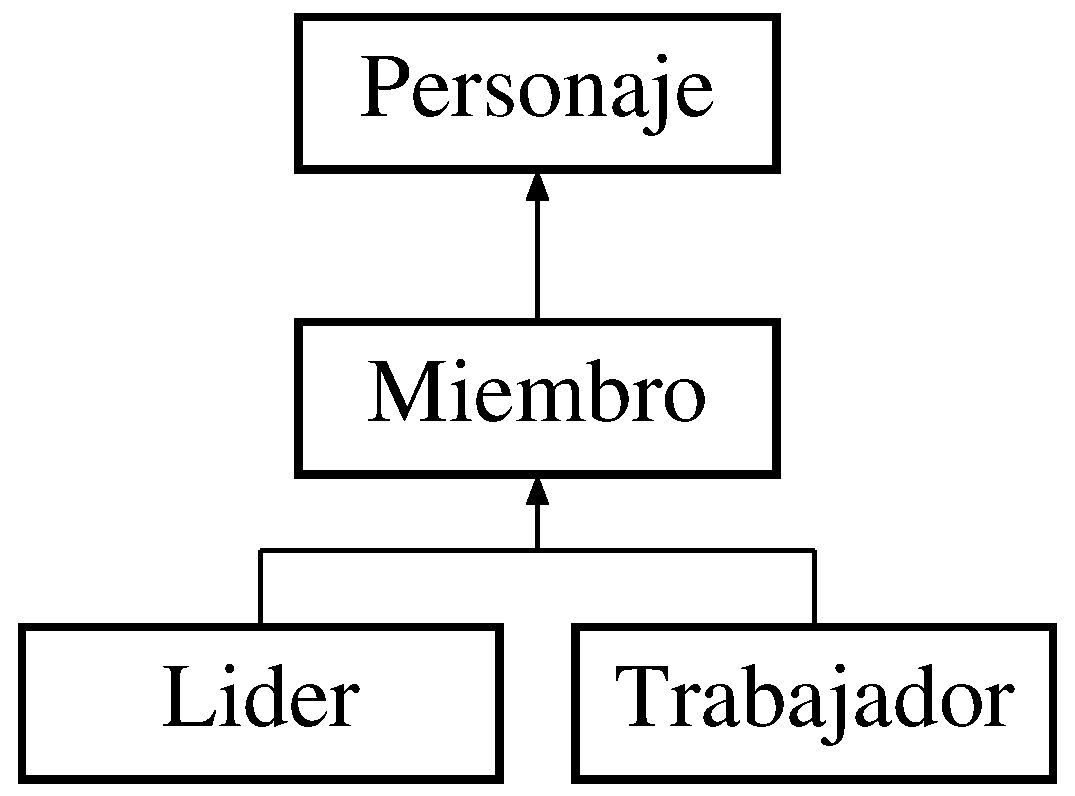
\includegraphics[height=3cm]{classMiembro}
\end{center}
\end{figure}
\subsection*{Public Member Functions}
\begin{CompactItemize}
\item 
\hyperlink{classMiembro_d5ad341737a1f4631694393c99204d91}{Miembro} ()
\item 
\hyperlink{classMiembro_d90b29c63638e16aa8f83f978cb7ec47}{Miembro} (char m, string n, int t, int ids, int idp)
\item 
void \hyperlink{classMiembro_28498c7229e81e64d0cb7ea69515dca0}{mostrar} ()
\item 
void \hyperlink{classMiembro_b286484cab275d7754c6ce2b513fdc9a}{accionCuatro} ()
\item 
\hyperlink{classMiembro_d8af12663ae1b9a195d05b4f700726c3}{$\sim$Miembro} ()
\end{CompactItemize}


\subsection{Detailed Description}
\begin{Desc}
\item[Author:]Carlos,,, $<$carlos-linux$>$ \end{Desc}


\subsection{Constructor \& Destructor Documentation}
\hypertarget{classMiembro_d5ad341737a1f4631694393c99204d91}{
\index{Miembro@{Miembro}!Miembro@{Miembro}}
\index{Miembro@{Miembro}!Miembro@{Miembro}}
\subsubsection[Miembro]{\setlength{\rightskip}{0pt plus 5cm}Miembro::Miembro ()}}
\label{classMiembro_d5ad341737a1f4631694393c99204d91}


Constructor por defecto de mi clase \hyperlink{classMiembro}{Miembro} \begin{Desc}
\item[Parameters:]
\begin{description}
\item[{\em \char`\"{}\char`\"{}}]no recibe parametros \end{description}
\end{Desc}
\begin{Desc}
\item[Returns:]No retorna ningun valor \end{Desc}
\hypertarget{classMiembro_d90b29c63638e16aa8f83f978cb7ec47}{
\index{Miembro@{Miembro}!Miembro@{Miembro}}
\index{Miembro@{Miembro}!Miembro@{Miembro}}
\subsubsection[Miembro]{\setlength{\rightskip}{0pt plus 5cm}Miembro::Miembro (char {\em m}, \/  string {\em n}, \/  int {\em t}, \/  int {\em ids}, \/  int {\em idp})}}
\label{classMiembro_d90b29c63638e16aa8f83f978cb7ec47}


Constructor parametrizado de mi clase miembro \begin{Desc}
\item[Parameters:]
\begin{description}
\item[{\em m}]es un parametro de entrada del tipo char correspondiente al atributo movimiento de mi clase \hyperlink{classPersonaje}{Personaje} \item[{\em n}]es un parametro de entrada del tipo string correspondiente al atributo nombre de mi clase \hyperlink{classPersonaje}{Personaje} \item[{\em t}]es un parametro de entrada del tipo entero correspondiente al atributo turno de mi clase \hyperlink{classPersonaje}{Personaje} \item[{\em ids}]es un parametro de entrada del tipo entero correspondiente al atributo idsala de mi clase \hyperlink{classPersonaje}{Personaje} \item[{\em idp}]es un parametro de entrada del tipo entero correspondiente al atributo idplanta de mi clase \hyperlink{classPersonaje}{Personaje} \end{description}
\end{Desc}
\begin{Desc}
\item[Returns:]No retorna ningun valor \end{Desc}
\hypertarget{classMiembro_d8af12663ae1b9a195d05b4f700726c3}{
\index{Miembro@{Miembro}!$\sim$Miembro@{$\sim$Miembro}}
\index{$\sim$Miembro@{$\sim$Miembro}!Miembro@{Miembro}}
\subsubsection[$\sim$Miembro]{\setlength{\rightskip}{0pt plus 5cm}Miembro::$\sim$Miembro ()}}
\label{classMiembro_d8af12663ae1b9a195d05b4f700726c3}


Destructor de mi clase \hyperlink{classMiembro}{Miembro} \begin{Desc}
\item[Parameters:]
\begin{description}
\item[{\em \char`\"{}\char`\"{}}]no recibe parametros \end{description}
\end{Desc}
\begin{Desc}
\item[Returns:]No retorna ningun valor \end{Desc}


\subsection{Member Function Documentation}
\hypertarget{classMiembro_28498c7229e81e64d0cb7ea69515dca0}{
\index{Miembro@{Miembro}!mostrar@{mostrar}}
\index{mostrar@{mostrar}!Miembro@{Miembro}}
\subsubsection[mostrar]{\setlength{\rightskip}{0pt plus 5cm}void Miembro::mostrar ()\hspace{0.3cm}{\tt  \mbox{[}virtual\mbox{]}}}}
\label{classMiembro_28498c7229e81e64d0cb7ea69515dca0}


Metodo que muestra por pantalla que el personaje es de tipo miembro \begin{Desc}
\item[Parameters:]
\begin{description}
\item[{\em \char`\"{}\char`\"{}}]no recibe parametros \end{description}
\end{Desc}
\begin{Desc}
\item[Returns:]No retorna ningun valor \end{Desc}


Reimplemented from \hyperlink{classPersonaje_e9f6bd8027b8a5c2e660a327d9e513ca}{Personaje}.

Reimplemented in \hyperlink{classLider_125acbb3a1432f217efdc9826a2b8d8f}{Lider}, and \hyperlink{classTrabajador_49e5a94181d6a517d9f5213335da1e27}{Trabajador}.\hypertarget{classMiembro_b286484cab275d7754c6ce2b513fdc9a}{
\index{Miembro@{Miembro}!accionCuatro@{accionCuatro}}
\index{accionCuatro@{accionCuatro}!Miembro@{Miembro}}
\subsubsection[accionCuatro]{\setlength{\rightskip}{0pt plus 5cm}void Miembro::accionCuatro ()\hspace{0.3cm}{\tt  \mbox{[}virtual\mbox{]}}}}
\label{classMiembro_b286484cab275d7754c6ce2b513fdc9a}


Metodo que realiza la accion cuatro de la clase miembro (lider y trabajador) \begin{Desc}
\item[Parameters:]
\begin{description}
\item[{\em \char`\"{}\char`\"{}}]no recibe parametros \end{description}
\end{Desc}
\begin{Desc}
\item[Returns:]No retorna ningun valor \end{Desc}


Reimplemented from \hyperlink{classPersonaje_3aed5959a6a829819e0b0a6dcca9c2e4}{Personaje}.

The documentation for this class was generated from the following files:\begin{CompactItemize}
\item 
Desktop/academia\_\-lp2/EC3\_\-LPII/src/miembro.h\item 
Desktop/academia\_\-lp2/EC3\_\-LPII/src/miembro.cpp\end{CompactItemize}

\hypertarget{classPersonaje}{
\section{Personaje Class Reference}
\label{classPersonaje}\index{Personaje@{Personaje}}
}
{\tt \#include $<$personaje.h$>$}

Inheritance diagram for Personaje::\begin{figure}[H]
\begin{center}
\leavevmode
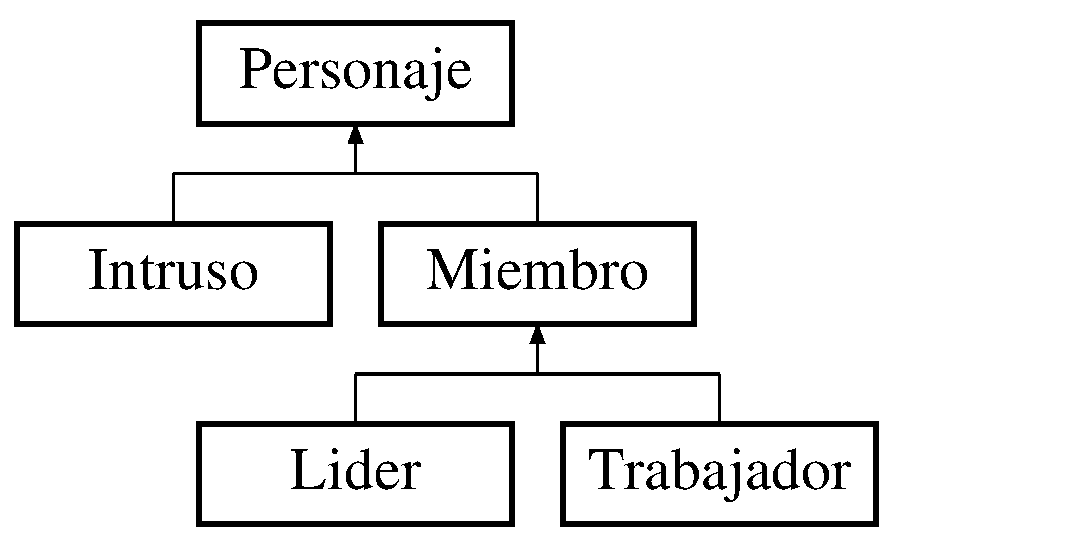
\includegraphics[height=3cm]{classPersonaje}
\end{center}
\end{figure}
\subsection*{Public Member Functions}
\begin{CompactItemize}
\item 
\hyperlink{classPersonaje_9238a75aae652b20dd423e85cfa1ee17}{Personaje} ()
\item 
\hyperlink{classPersonaje_a86eafddc218e8afa94f989b3642bcbd}{Personaje} (char m, string n, int t, int ids, int idp)
\item 
void \hyperlink{classPersonaje_475630fe753b7fb80a2472c558d99169}{setMarca} (char m)
\item 
char \hyperlink{classPersonaje_36e1ba57799adb58163bec5a4f0015e0}{getMarca} ()
\item 
void \hyperlink{classPersonaje_2e84ee485f46b434f1d23558ad3eb7c9}{setNombre} (string n)
\item 
void \hyperlink{classPersonaje_801e7fe38d0727d3219e51e916e2ce67}{getNombre} (string \&n)
\item 
void \hyperlink{classPersonaje_de04da7a674a165aeaa09566b219a828}{setTurno} (int t)
\item 
int \hyperlink{classPersonaje_425c743df0309deab48e9575d715eed9}{getTurno} ()
\item 
void \hyperlink{classPersonaje_43a551a88fe3c6d4458719135992114b}{setIdSala} (int ids)
\item 
int \hyperlink{classPersonaje_5266df5bdfa75df5dfc631d94be2993d}{getIdSala} ()
\item 
void \hyperlink{classPersonaje_361e72e69c915f6e0c7d2c5e82ae0744}{setIdPlanta} (int idp)
\item 
int \hyperlink{classPersonaje_f388d329d466b136c60fa26c6c4800a7}{getIdPlanta} ()
\item 
void \hyperlink{classPersonaje_1ad939228d858b75826ddb4effa67ceb}{liberarMemoriaPila} (stack$<$ \hyperlink{classLlave}{Llave} $\ast$ $>$ $\ast$\&lis)
\item 
void \hyperlink{classPersonaje_6ede7d70599342ba61eb034027a41f2a}{insertarPila} (\hyperlink{classLlave}{Llave} $\ast$l)
\item 
void \hyperlink{classPersonaje_8880afa570d1f919516e2810b2226b08}{cojerLlave} (\hyperlink{classLlave}{Llave} $\ast$\&l)
\item 
bool \hyperlink{classPersonaje_27166f7a52fcfb3570e0dc20f37a2402}{pilaVacia} ()
\item 
void \hyperlink{classPersonaje_66ec23478444efc795d29734cc010809}{insertarCola} (int i)
\item 
void \hyperlink{classPersonaje_786951aff09e227527d3da60338effec}{TodasAcciones} ()
\item 
virtual void \hyperlink{classPersonaje_0454b75ccc8f7e33f03e2cfb2c59e725}{accionUno} ()
\item 
virtual void \hyperlink{classPersonaje_af7763eb6099390038b7833129a1ef9f}{accionDos} ()
\item 
virtual void \hyperlink{classPersonaje_85c25ff0362bf4f4f5e69965c1ae4cfb}{accionTres} ()
\item 
virtual void \hyperlink{classPersonaje_3aed5959a6a829819e0b0a6dcca9c2e4}{accionCuatro} ()
\item 
virtual void \hyperlink{classPersonaje_f6dc20013805229005dfb87fc6f273b5}{ruta} (ofstream \&f)
\item 
virtual void \hyperlink{classPersonaje_86fe4a1ff708072d98c6be42bbd512ea}{escribeLog} (ofstream \&f)
\item 
virtual void \hyperlink{classPersonaje_e9f6bd8027b8a5c2e660a327d9e513ca}{mostrar} ()
\item 
virtual \hyperlink{classPersonaje_0b3c25862a6081aaee96e77c08edda29}{$\sim$Personaje} ()
\item 
int \hyperlink{classPersonaje_5870893672c215b1d99594233f7f5fd0}{operator==} (\hyperlink{classPersonaje}{Personaje} \&p)
\item 
int \hyperlink{classPersonaje_7717f9a6ad3d7b68a5c953930510f575}{operator$>$} (\hyperlink{classPersonaje}{Personaje} \&p)
\item 
int \hyperlink{classPersonaje_e55182c2fd21118b27c5e911f800c1d6}{operator$<$} (\hyperlink{classPersonaje}{Personaje} \&p)
\item 
int \hyperlink{classPersonaje_5b7fbb10c092e6f953738fa54a380e33}{operator$>$=} (\hyperlink{classPersonaje}{Personaje} \&p)
\item 
int \hyperlink{classPersonaje_824156240864cc79a8b7319985eaec58}{operator$<$=} (\hyperlink{classPersonaje}{Personaje} \&p)
\item 
int \hyperlink{classPersonaje_be7f26619dd67133806688d4306d877e}{operator!=} (\hyperlink{classPersonaje}{Personaje} \&p)
\end{CompactItemize}
\subsection*{Protected Attributes}
\begin{CompactItemize}
\item 
\hypertarget{classPersonaje_8f20063ad43d9f85a6d1f0022d32e0b4}{
char \textbf{marca}}
\label{classPersonaje_8f20063ad43d9f85a6d1f0022d32e0b4}

\item 
\hypertarget{classPersonaje_0c1fedf7d7ec93a6ca1d38aa6a79b7e2}{
string \textbf{nombre}}
\label{classPersonaje_0c1fedf7d7ec93a6ca1d38aa6a79b7e2}

\item 
\hypertarget{classPersonaje_0bce8e11746271ccf72035ea3da1138e}{
int \textbf{turno}}
\label{classPersonaje_0bce8e11746271ccf72035ea3da1138e}

\item 
\hypertarget{classPersonaje_31a8a079b785a74622cc8dd51a9f745c}{
int \textbf{idsala}}
\label{classPersonaje_31a8a079b785a74622cc8dd51a9f745c}

\item 
\hypertarget{classPersonaje_8160f258ed0b5836b1173cbef638bde3}{
int \textbf{idplanta}}
\label{classPersonaje_8160f258ed0b5836b1173cbef638bde3}

\item 
\hypertarget{classPersonaje_ea1a86738c789e65792ed745039bce46}{
queue$<$ int $>$ \textbf{secuencia}}
\label{classPersonaje_ea1a86738c789e65792ed745039bce46}

\item 
\hypertarget{classPersonaje_e98a94dc9f84d09e3a62266d5cac700c}{
stack$<$ \hyperlink{classLlave}{Llave} $\ast$ $>$ $\ast$ \textbf{juegollaves}}
\label{classPersonaje_e98a94dc9f84d09e3a62266d5cac700c}

\end{CompactItemize}


\subsection{Detailed Description}
\begin{Desc}
\item[Author:]Carlos,,, $<$carlos-linux$>$ \end{Desc}


\subsection{Constructor \& Destructor Documentation}
\hypertarget{classPersonaje_9238a75aae652b20dd423e85cfa1ee17}{
\index{Personaje@{Personaje}!Personaje@{Personaje}}
\index{Personaje@{Personaje}!Personaje@{Personaje}}
\subsubsection[Personaje]{\setlength{\rightskip}{0pt plus 5cm}Personaje::Personaje ()}}
\label{classPersonaje_9238a75aae652b20dd423e85cfa1ee17}


Constructor por defecto de mi clase \hyperlink{classPersonaje}{Personaje} \begin{Desc}
\item[Parameters:]
\begin{description}
\item[{\em \char`\"{}\char`\"{}}]no recibe parametros \end{description}
\end{Desc}
\begin{Desc}
\item[Returns:]No retorna ningun valor \end{Desc}
\hypertarget{classPersonaje_a86eafddc218e8afa94f989b3642bcbd}{
\index{Personaje@{Personaje}!Personaje@{Personaje}}
\index{Personaje@{Personaje}!Personaje@{Personaje}}
\subsubsection[Personaje]{\setlength{\rightskip}{0pt plus 5cm}Personaje::Personaje (char {\em m}, \/  string {\em n}, \/  int {\em t}, \/  int {\em ids}, \/  int {\em idp})}}
\label{classPersonaje_a86eafddc218e8afa94f989b3642bcbd}


Constructor parametrizado de mi clase \hyperlink{classPersonaje}{Personaje} \begin{Desc}
\item[Parameters:]
\begin{description}
\item[{\em m}]es un parametro de entrada del tipo char asociado al atributo movimiento de mi clase \hyperlink{classPersonaje}{Personaje} \item[{\em n}]es un parametro de entrada del tipo string asociado al atributo nombre de mi clase \hyperlink{classPersonaje}{Personaje} \item[{\em t}]es un parametro de entrada del tipo entero asociado al atributo turno de mi clase \hyperlink{classPersonaje}{Personaje} \item[{\em ids}]es un parametro de entrada del tipo entero asociado al atributo idsala de mi clase \hyperlink{classPersonaje}{Personaje} \item[{\em idp}]es un parametro de entrada del tipo entero asociado al atributo idplanta de mi clase \hyperlink{classPersonaje}{Personaje} \end{description}
\end{Desc}
\begin{Desc}
\item[Returns:]No retorna ningun valor \end{Desc}
\hypertarget{classPersonaje_0b3c25862a6081aaee96e77c08edda29}{
\index{Personaje@{Personaje}!$\sim$Personaje@{$\sim$Personaje}}
\index{$\sim$Personaje@{$\sim$Personaje}!Personaje@{Personaje}}
\subsubsection[$\sim$Personaje]{\setlength{\rightskip}{0pt plus 5cm}Personaje::$\sim$Personaje ()\hspace{0.3cm}{\tt  \mbox{[}virtual\mbox{]}}}}
\label{classPersonaje_0b3c25862a6081aaee96e77c08edda29}


Destructor de mi clase \hyperlink{classPersonaje}{Personaje} \begin{Desc}
\item[Parameters:]
\begin{description}
\item[{\em \char`\"{}\char`\"{}}]no recibe parametros \end{description}
\end{Desc}
\begin{Desc}
\item[Returns:]No retorna ningun valor \end{Desc}


\subsection{Member Function Documentation}
\hypertarget{classPersonaje_475630fe753b7fb80a2472c558d99169}{
\index{Personaje@{Personaje}!setMarca@{setMarca}}
\index{setMarca@{setMarca}!Personaje@{Personaje}}
\subsubsection[setMarca]{\setlength{\rightskip}{0pt plus 5cm}void Personaje::setMarca (char {\em m})}}
\label{classPersonaje_475630fe753b7fb80a2472c558d99169}


Metodo que establece al atributo movimiento de mi clase personaje el valor de m \begin{Desc}
\item[Parameters:]
\begin{description}
\item[{\em m}]es un parametro de entrada del tipo char \end{description}
\end{Desc}
\begin{Desc}
\item[Returns:]No retorna ningun valor \end{Desc}
\hypertarget{classPersonaje_36e1ba57799adb58163bec5a4f0015e0}{
\index{Personaje@{Personaje}!getMarca@{getMarca}}
\index{getMarca@{getMarca}!Personaje@{Personaje}}
\subsubsection[getMarca]{\setlength{\rightskip}{0pt plus 5cm}char Personaje::getMarca ()}}
\label{classPersonaje_36e1ba57799adb58163bec5a4f0015e0}


Metodo que devuelve el caracter asociado al atributo movimiento de mi clase \hyperlink{classPersonaje}{Personaje} \begin{Desc}
\item[Parameters:]
\begin{description}
\item[{\em \char`\"{}\char`\"{}}]no recibe parametros \end{description}
\end{Desc}
\begin{Desc}
\item[Returns:]Retorna el char correspondiente al atributo movimiento de mi clase \hyperlink{classPersonaje}{Personaje} \end{Desc}
\hypertarget{classPersonaje_2e84ee485f46b434f1d23558ad3eb7c9}{
\index{Personaje@{Personaje}!setNombre@{setNombre}}
\index{setNombre@{setNombre}!Personaje@{Personaje}}
\subsubsection[setNombre]{\setlength{\rightskip}{0pt plus 5cm}void Personaje::setNombre (string {\em n})}}
\label{classPersonaje_2e84ee485f46b434f1d23558ad3eb7c9}


Metodo que establece el valor de mi atributo de tipo string, nombre, de mi clase \hyperlink{classPersonaje}{Personaje} \begin{Desc}
\item[Parameters:]
\begin{description}
\item[{\em n}]es un parametro de entrada del tipo string asociado al atributo nombre de mi clase \hyperlink{classPersonaje}{Personaje} \end{description}
\end{Desc}
\begin{Desc}
\item[Returns:]No retorna ningun valor \end{Desc}
\hypertarget{classPersonaje_801e7fe38d0727d3219e51e916e2ce67}{
\index{Personaje@{Personaje}!getNombre@{getNombre}}
\index{getNombre@{getNombre}!Personaje@{Personaje}}
\subsubsection[getNombre]{\setlength{\rightskip}{0pt plus 5cm}void Personaje::getNombre (string \& {\em n})}}
\label{classPersonaje_801e7fe38d0727d3219e51e916e2ce67}


Metodo que devuelve el contenido del atributo nombre de mi clase \hyperlink{classPersonaje}{Personaje} \begin{Desc}
\item[Parameters:]
\begin{description}
\item[{\em n}]es un parametro salida que devuelve el contenido de mi atributo nombre de mi clase \hyperlink{classPersonaje}{Personaje} \end{description}
\end{Desc}
\begin{Desc}
\item[Returns:]No retorna ningun valor \end{Desc}
\hypertarget{classPersonaje_de04da7a674a165aeaa09566b219a828}{
\index{Personaje@{Personaje}!setTurno@{setTurno}}
\index{setTurno@{setTurno}!Personaje@{Personaje}}
\subsubsection[setTurno]{\setlength{\rightskip}{0pt plus 5cm}void Personaje::setTurno (int {\em t})}}
\label{classPersonaje_de04da7a674a165aeaa09566b219a828}


Metodo que establece el valor de mi atributo turno de mi clase \hyperlink{classPersonaje}{Personaje} \begin{Desc}
\item[Parameters:]
\begin{description}
\item[{\em t}]es un parametro de entrada del tipo entero \end{description}
\end{Desc}
\begin{Desc}
\item[Returns:]No retorna ningun valor \end{Desc}
\hypertarget{classPersonaje_425c743df0309deab48e9575d715eed9}{
\index{Personaje@{Personaje}!getTurno@{getTurno}}
\index{getTurno@{getTurno}!Personaje@{Personaje}}
\subsubsection[getTurno]{\setlength{\rightskip}{0pt plus 5cm}int Personaje::getTurno ()}}
\label{classPersonaje_425c743df0309deab48e9575d715eed9}


Metodo que devuelve el valor del atributo turno de mi clase \hyperlink{classPersonaje}{Personaje} \begin{Desc}
\item[Parameters:]
\begin{description}
\item[{\em \char`\"{}\char`\"{}}]no recibe parametros \end{description}
\end{Desc}
\begin{Desc}
\item[Returns:]Devuelve el entero correspondiente al valor de mi atributo turno de mi clase \hyperlink{classPersonaje}{Personaje} \end{Desc}
\hypertarget{classPersonaje_43a551a88fe3c6d4458719135992114b}{
\index{Personaje@{Personaje}!setIdSala@{setIdSala}}
\index{setIdSala@{setIdSala}!Personaje@{Personaje}}
\subsubsection[setIdSala]{\setlength{\rightskip}{0pt plus 5cm}void Personaje::setIdSala (int {\em ids})}}
\label{classPersonaje_43a551a88fe3c6d4458719135992114b}


Metodo que establece el valor de mi atributo idsala de mi clase \hyperlink{classPersonaje}{Personaje} \begin{Desc}
\item[Parameters:]
\begin{description}
\item[{\em ids}]es un parametro de entrada del tipo entero \end{description}
\end{Desc}
\begin{Desc}
\item[Returns:]No retorna ningun valor \end{Desc}
\hypertarget{classPersonaje_5266df5bdfa75df5dfc631d94be2993d}{
\index{Personaje@{Personaje}!getIdSala@{getIdSala}}
\index{getIdSala@{getIdSala}!Personaje@{Personaje}}
\subsubsection[getIdSala]{\setlength{\rightskip}{0pt plus 5cm}int Personaje::getIdSala ()}}
\label{classPersonaje_5266df5bdfa75df5dfc631d94be2993d}


Metodo que devuelve el valor asociado a mi atributo idsala de mi clase \hyperlink{classPersonaje}{Personaje} \begin{Desc}
\item[Parameters:]
\begin{description}
\item[{\em \char`\"{}\char`\"{}}]no recibe parametros \end{description}
\end{Desc}
\begin{Desc}
\item[Returns:]Retorna el valor correspondiente al atributo idsala de mi clase \hyperlink{classPersonaje}{Personaje} \end{Desc}
\hypertarget{classPersonaje_361e72e69c915f6e0c7d2c5e82ae0744}{
\index{Personaje@{Personaje}!setIdPlanta@{setIdPlanta}}
\index{setIdPlanta@{setIdPlanta}!Personaje@{Personaje}}
\subsubsection[setIdPlanta]{\setlength{\rightskip}{0pt plus 5cm}void Personaje::setIdPlanta (int {\em idp})}}
\label{classPersonaje_361e72e69c915f6e0c7d2c5e82ae0744}


Metodo que establece el valor de mi atributo idplanta de mi clase \hyperlink{classPersonaje}{Personaje} \begin{Desc}
\item[Parameters:]
\begin{description}
\item[{\em idp}]es un parametro de entrada del tipo entero \end{description}
\end{Desc}
\begin{Desc}
\item[Returns:]No retorna ningun valor \end{Desc}
\hypertarget{classPersonaje_f388d329d466b136c60fa26c6c4800a7}{
\index{Personaje@{Personaje}!getIdPlanta@{getIdPlanta}}
\index{getIdPlanta@{getIdPlanta}!Personaje@{Personaje}}
\subsubsection[getIdPlanta]{\setlength{\rightskip}{0pt plus 5cm}int Personaje::getIdPlanta ()}}
\label{classPersonaje_f388d329d466b136c60fa26c6c4800a7}


Metodo que devuelve el valor correspondiente con el atributo idplanta de mi clase \hyperlink{classPersonaje}{Personaje} \begin{Desc}
\item[Parameters:]
\begin{description}
\item[{\em \char`\"{}\char`\"{}}]no recibe parametros \end{description}
\end{Desc}
\begin{Desc}
\item[Returns:]No retorna ningun valor \end{Desc}
\hypertarget{classPersonaje_1ad939228d858b75826ddb4effa67ceb}{
\index{Personaje@{Personaje}!liberarMemoriaPila@{liberarMemoriaPila}}
\index{liberarMemoriaPila@{liberarMemoriaPila}!Personaje@{Personaje}}
\subsubsection[liberarMemoriaPila]{\setlength{\rightskip}{0pt plus 5cm}void Personaje::liberarMemoriaPila (stack$<$ {\bf Llave} $\ast$ $>$ $\ast$\& {\em pil})}}
\label{classPersonaje_1ad939228d858b75826ddb4effa67ceb}


Metodo que libera la memoria de cada \hyperlink{classLlave}{Llave} contenida en mi estructura pila pil \begin{Desc}
\item[Parameters:]
\begin{description}
\item[{\em pil}]es un parametro de entrada salida (puntero) que almacena punteros a instancias de mi clase \hyperlink{classLlave}{Llave} \end{description}
\end{Desc}
\begin{Desc}
\item[Returns:]No retorna ningun valor \end{Desc}
\hypertarget{classPersonaje_6ede7d70599342ba61eb034027a41f2a}{
\index{Personaje@{Personaje}!insertarPila@{insertarPila}}
\index{insertarPila@{insertarPila}!Personaje@{Personaje}}
\subsubsection[insertarPila]{\setlength{\rightskip}{0pt plus 5cm}void Personaje::insertarPila ({\bf Llave} $\ast$ {\em l})}}
\label{classPersonaje_6ede7d70599342ba61eb034027a41f2a}


Metodo que inserta en mi atributo juegollaves del tipo pila un puntero a una instancia de mi clase \hyperlink{classLlave}{Llave} \begin{Desc}
\item[Parameters:]
\begin{description}
\item[{\em l}]es un parametro de entrada de mi clase \hyperlink{classLlave}{Llave} \end{description}
\end{Desc}
\begin{Desc}
\item[Returns:]No retorna ningun valor \end{Desc}
\hypertarget{classPersonaje_8880afa570d1f919516e2810b2226b08}{
\index{Personaje@{Personaje}!cojerLlave@{cojerLlave}}
\index{cojerLlave@{cojerLlave}!Personaje@{Personaje}}
\subsubsection[cojerLlave]{\setlength{\rightskip}{0pt plus 5cm}void Personaje::cojerLlave ({\bf Llave} $\ast$\& {\em l})}}
\label{classPersonaje_8880afa570d1f919516e2810b2226b08}


Metodo que devuelve la primera llave de mi atributo del tipo pila juegollaves si la cola no esta vacia y ademas ,desapila esa llave \begin{Desc}
\item[Parameters:]
\begin{description}
\item[{\em l}]es un parametro de entrada salida de mi clase \hyperlink{classLlave}{Llave} \end{description}
\end{Desc}
\begin{Desc}
\item[Returns:]No retorna ningun valor \end{Desc}
\hypertarget{classPersonaje_27166f7a52fcfb3570e0dc20f37a2402}{
\index{Personaje@{Personaje}!pilaVacia@{pilaVacia}}
\index{pilaVacia@{pilaVacia}!Personaje@{Personaje}}
\subsubsection[pilaVacia]{\setlength{\rightskip}{0pt plus 5cm}bool Personaje::pilaVacia ()}}
\label{classPersonaje_27166f7a52fcfb3570e0dc20f37a2402}


Metodo booleano que me indica si mi atributo del tipo pila juegollaves se encuentra vacia o no \begin{Desc}
\item[Parameters:]
\begin{description}
\item[{\em \char`\"{}\char`\"{}}]no recibe parametros \end{description}
\end{Desc}
\begin{Desc}
\item[Returns:]Retorna true si la pila esta vacia y false en caso contrario \end{Desc}
\hypertarget{classPersonaje_66ec23478444efc795d29734cc010809}{
\index{Personaje@{Personaje}!insertarCola@{insertarCola}}
\index{insertarCola@{insertarCola}!Personaje@{Personaje}}
\subsubsection[insertarCola]{\setlength{\rightskip}{0pt plus 5cm}void Personaje::insertarCola (int {\em i})}}
\label{classPersonaje_66ec23478444efc795d29734cc010809}


Metodo que inserta en mi cola secuencia un valor entero \begin{Desc}
\item[Parameters:]
\begin{description}
\item[{\em i}]es un parametro de entrada del tipo entero \end{description}
\end{Desc}
\begin{Desc}
\item[Returns:]No retorna ningun valor \end{Desc}
\hypertarget{classPersonaje_786951aff09e227527d3da60338effec}{
\index{Personaje@{Personaje}!TodasAcciones@{TodasAcciones}}
\index{TodasAcciones@{TodasAcciones}!Personaje@{Personaje}}
\subsubsection[TodasAcciones]{\setlength{\rightskip}{0pt plus 5cm}void Personaje::TodasAcciones ()}}
\label{classPersonaje_786951aff09e227527d3da60338effec}


Metodo que realiza todas las acciones (uno,dos,tres y cuatro) de la clase \hyperlink{classPersonaje}{Personaje} \begin{Desc}
\item[Parameters:]
\begin{description}
\item[{\em \char`\"{}\char`\"{}}]no recibe parametros \end{description}
\end{Desc}
\begin{Desc}
\item[Returns:]No retorna ningun valor \end{Desc}
\hypertarget{classPersonaje_0454b75ccc8f7e33f03e2cfb2c59e725}{
\index{Personaje@{Personaje}!accionUno@{accionUno}}
\index{accionUno@{accionUno}!Personaje@{Personaje}}
\subsubsection[accionUno]{\setlength{\rightskip}{0pt plus 5cm}void Personaje::accionUno ()\hspace{0.3cm}{\tt  \mbox{[}virtual\mbox{]}}}}
\label{classPersonaje_0454b75ccc8f7e33f03e2cfb2c59e725}


Metodo que realiza la accion uno de la clase \hyperlink{classPersonaje}{Personaje} \begin{Desc}
\item[Parameters:]
\begin{description}
\item[{\em \char`\"{}\char`\"{}}]no recibe parametros \end{description}
\end{Desc}
\begin{Desc}
\item[Returns:]No retorna ningun valor \end{Desc}


Reimplemented in \hyperlink{classIntruso_dee71b00225e294086d8980625a32ab3}{Intruso}, \hyperlink{classLider_2729cb612e6ca2d2750f48b85743107e}{Lider}, and \hyperlink{classTrabajador_ea6e8089295c87f0b5a5014895f28526}{Trabajador}.\hypertarget{classPersonaje_af7763eb6099390038b7833129a1ef9f}{
\index{Personaje@{Personaje}!accionDos@{accionDos}}
\index{accionDos@{accionDos}!Personaje@{Personaje}}
\subsubsection[accionDos]{\setlength{\rightskip}{0pt plus 5cm}void Personaje::accionDos ()\hspace{0.3cm}{\tt  \mbox{[}virtual\mbox{]}}}}
\label{classPersonaje_af7763eb6099390038b7833129a1ef9f}


Metodo que realiza la accion dos de la clase \hyperlink{classPersonaje}{Personaje} \begin{Desc}
\item[Parameters:]
\begin{description}
\item[{\em \char`\"{}\char`\"{}}]no recibe parametros \end{description}
\end{Desc}
\begin{Desc}
\item[Returns:]No retorna ningun valor \end{Desc}


Reimplemented in \hyperlink{classIntruso_6fef0ae823fdabc05796413f53d073e5}{Intruso}, \hyperlink{classLider_51fb2d9c6dfe283a13d61b8f546068f3}{Lider}, and \hyperlink{classTrabajador_598df69f74628e4da5d0dc776c98b114}{Trabajador}.\hypertarget{classPersonaje_85c25ff0362bf4f4f5e69965c1ae4cfb}{
\index{Personaje@{Personaje}!accionTres@{accionTres}}
\index{accionTres@{accionTres}!Personaje@{Personaje}}
\subsubsection[accionTres]{\setlength{\rightskip}{0pt plus 5cm}void Personaje::accionTres ()\hspace{0.3cm}{\tt  \mbox{[}virtual\mbox{]}}}}
\label{classPersonaje_85c25ff0362bf4f4f5e69965c1ae4cfb}


Metodo que realiza la accion tres de la clase \hyperlink{classPersonaje}{Personaje} \begin{Desc}
\item[Parameters:]
\begin{description}
\item[{\em \char`\"{}\char`\"{}}]no recibe parametros \end{description}
\end{Desc}
\begin{Desc}
\item[Returns:]No retorna ningun valor \end{Desc}


Reimplemented in \hyperlink{classIntruso_52e521cc66983d5a9f20f3424818e6e4}{Intruso}, \hyperlink{classLider_993a29f5a5615bd8a41dfe550dfccb61}{Lider}, and \hyperlink{classTrabajador_9203576ae93a8854b033f1d91e25fee7}{Trabajador}.\hypertarget{classPersonaje_3aed5959a6a829819e0b0a6dcca9c2e4}{
\index{Personaje@{Personaje}!accionCuatro@{accionCuatro}}
\index{accionCuatro@{accionCuatro}!Personaje@{Personaje}}
\subsubsection[accionCuatro]{\setlength{\rightskip}{0pt plus 5cm}void Personaje::accionCuatro ()\hspace{0.3cm}{\tt  \mbox{[}virtual\mbox{]}}}}
\label{classPersonaje_3aed5959a6a829819e0b0a6dcca9c2e4}


Metodo que realiza la accion cuatro de la clase \hyperlink{classPersonaje}{Personaje} \begin{Desc}
\item[Parameters:]
\begin{description}
\item[{\em \char`\"{}\char`\"{}}]no recibe parametros \end{description}
\end{Desc}
\begin{Desc}
\item[Returns:]No retorna ningun valor \end{Desc}


Reimplemented in \hyperlink{classIntruso_99e215b1df4387b629f25349378d3bbb}{Intruso}, and \hyperlink{classMiembro_b286484cab275d7754c6ce2b513fdc9a}{Miembro}.\hypertarget{classPersonaje_f6dc20013805229005dfb87fc6f273b5}{
\index{Personaje@{Personaje}!ruta@{ruta}}
\index{ruta@{ruta}!Personaje@{Personaje}}
\subsubsection[ruta]{\setlength{\rightskip}{0pt plus 5cm}void Personaje::ruta (ofstream \& {\em f})\hspace{0.3cm}{\tt  \mbox{[}virtual\mbox{]}}}}
\label{classPersonaje_f6dc20013805229005dfb87fc6f273b5}


Metodo que realiza la ruta de mi clase \hyperlink{classPersonaje}{Personaje} \begin{Desc}
\item[Parameters:]
\begin{description}
\item[{\em f}]es un flujo de entrada salida \end{description}
\end{Desc}
\begin{Desc}
\item[Returns:]No retorna ningun valor \end{Desc}


Reimplemented in \hyperlink{classIntruso_2898ae82386e99d361f6f131122b7be1}{Intruso}, \hyperlink{classLider_6b98929df0d59cd29b85e6fb8aeb36f1}{Lider}, and \hyperlink{classTrabajador_6b940e57a18466eafa2dcfe0a60313d3}{Trabajador}.\hypertarget{classPersonaje_86fe4a1ff708072d98c6be42bbd512ea}{
\index{Personaje@{Personaje}!escribeLog@{escribeLog}}
\index{escribeLog@{escribeLog}!Personaje@{Personaje}}
\subsubsection[escribeLog]{\setlength{\rightskip}{0pt plus 5cm}void Personaje::escribeLog (ofstream \& {\em f})\hspace{0.3cm}{\tt  \mbox{[}virtual\mbox{]}}}}
\label{classPersonaje_86fe4a1ff708072d98c6be42bbd512ea}


Metodo escribe en mi registro.log de mi clase \hyperlink{classPersonaje}{Personaje} \begin{Desc}
\item[Parameters:]
\begin{description}
\item[{\em f}]es un flujo de entrada salida \end{description}
\end{Desc}
\begin{Desc}
\item[Returns:]No retorna ningun valor \end{Desc}


Reimplemented in \hyperlink{classIntruso_979c89c596d92d8ce69b8af5e556d62d}{Intruso}, \hyperlink{classLider_fcd179370f87dbc08bf6619ff9742f66}{Lider}, and \hyperlink{classTrabajador_332796b26094df07fa7b8b39c345f8f4}{Trabajador}.\hypertarget{classPersonaje_e9f6bd8027b8a5c2e660a327d9e513ca}{
\index{Personaje@{Personaje}!mostrar@{mostrar}}
\index{mostrar@{mostrar}!Personaje@{Personaje}}
\subsubsection[mostrar]{\setlength{\rightskip}{0pt plus 5cm}void Personaje::mostrar ()\hspace{0.3cm}{\tt  \mbox{[}virtual\mbox{]}}}}
\label{classPersonaje_e9f6bd8027b8a5c2e660a327d9e513ca}


Metodo que muestra por pantalla que el personaje es del tipo personaje \begin{Desc}
\item[Parameters:]
\begin{description}
\item[{\em \char`\"{}\char`\"{}}]no recibe parametros \end{description}
\end{Desc}
\begin{Desc}
\item[Returns:]No retorna ningun valor \end{Desc}


Reimplemented in \hyperlink{classIntruso_06a5d236e669e5add8b1c6472303133e}{Intruso}, \hyperlink{classLider_125acbb3a1432f217efdc9826a2b8d8f}{Lider}, \hyperlink{classMiembro_28498c7229e81e64d0cb7ea69515dca0}{Miembro}, and \hyperlink{classTrabajador_49e5a94181d6a517d9f5213335da1e27}{Trabajador}.\hypertarget{classPersonaje_5870893672c215b1d99594233f7f5fd0}{
\index{Personaje@{Personaje}!operator==@{operator==}}
\index{operator==@{operator==}!Personaje@{Personaje}}
\subsubsection[operator==]{\setlength{\rightskip}{0pt plus 5cm}int Personaje::operator== ({\bf Personaje} \& {\em p})}}
\label{classPersonaje_5870893672c215b1d99594233f7f5fd0}


Sobrecarga del operador \char`\"{}==\char`\"{} de mi clase \hyperlink{classPersonaje}{Personaje} \begin{Desc}
\item[Parameters:]
\begin{description}
\item[{\em p}]es un parametro de entrada salida de mi clase \hyperlink{classPersonaje}{Personaje} \end{description}
\end{Desc}
\begin{Desc}
\item[Returns:]No retorna ningun valor \end{Desc}
\hypertarget{classPersonaje_7717f9a6ad3d7b68a5c953930510f575}{
\index{Personaje@{Personaje}!operator$>$@{operator$>$}}
\index{operator$>$@{operator$>$}!Personaje@{Personaje}}
\subsubsection[operator$>$]{\setlength{\rightskip}{0pt plus 5cm}int Personaje::operator$>$ ({\bf Personaje} \& {\em p})}}
\label{classPersonaje_7717f9a6ad3d7b68a5c953930510f575}


Sobrecarga del operador \char`\"{}$>$\char`\"{} de mi clase \hyperlink{classPersonaje}{Personaje} \begin{Desc}
\item[Parameters:]
\begin{description}
\item[{\em p}]es un parametro de entrada salida de mi clase \hyperlink{classPersonaje}{Personaje} \end{description}
\end{Desc}
\begin{Desc}
\item[Returns:]No retorna ningun valor \end{Desc}
\hypertarget{classPersonaje_e55182c2fd21118b27c5e911f800c1d6}{
\index{Personaje@{Personaje}!operator$<$@{operator$<$}}
\index{operator$<$@{operator$<$}!Personaje@{Personaje}}
\subsubsection[operator$<$]{\setlength{\rightskip}{0pt plus 5cm}int Personaje::operator$<$ ({\bf Personaje} \& {\em p})}}
\label{classPersonaje_e55182c2fd21118b27c5e911f800c1d6}


Sobrecarga del operador \char`\"{}$<$\char`\"{} de mi clase \hyperlink{classPersonaje}{Personaje} \begin{Desc}
\item[Parameters:]
\begin{description}
\item[{\em p}]es un parametro de entrada salida de mi clase \hyperlink{classPersonaje}{Personaje} \end{description}
\end{Desc}
\begin{Desc}
\item[Returns:]No retorna ningun valor \end{Desc}
\hypertarget{classPersonaje_5b7fbb10c092e6f953738fa54a380e33}{
\index{Personaje@{Personaje}!operator$>$=@{operator$>$=}}
\index{operator$>$=@{operator$>$=}!Personaje@{Personaje}}
\subsubsection[operator$>$=]{\setlength{\rightskip}{0pt plus 5cm}int Personaje::operator$>$= ({\bf Personaje} \& {\em p})}}
\label{classPersonaje_5b7fbb10c092e6f953738fa54a380e33}


Sobrecarga del operador \char`\"{}$>$=\char`\"{} de mi clase \hyperlink{classPersonaje}{Personaje} \begin{Desc}
\item[Parameters:]
\begin{description}
\item[{\em p}]es un parametro de entrada salida de mi clase \hyperlink{classPersonaje}{Personaje} \end{description}
\end{Desc}
\begin{Desc}
\item[Returns:]No retorna ningun valor \end{Desc}
\hypertarget{classPersonaje_824156240864cc79a8b7319985eaec58}{
\index{Personaje@{Personaje}!operator$<$=@{operator$<$=}}
\index{operator$<$=@{operator$<$=}!Personaje@{Personaje}}
\subsubsection[operator$<$=]{\setlength{\rightskip}{0pt plus 5cm}int Personaje::operator$<$= ({\bf Personaje} \& {\em p})}}
\label{classPersonaje_824156240864cc79a8b7319985eaec58}


Sobrecarga del operador \char`\"{}$<$=\char`\"{} de mi clase \hyperlink{classPersonaje}{Personaje} \begin{Desc}
\item[Parameters:]
\begin{description}
\item[{\em p}]es un parametro de entrada salida de mi clase \hyperlink{classPersonaje}{Personaje} \end{description}
\end{Desc}
\begin{Desc}
\item[Returns:]No retorna ningun valor \end{Desc}
\hypertarget{classPersonaje_be7f26619dd67133806688d4306d877e}{
\index{Personaje@{Personaje}!operator"!=@{operator"!=}}
\index{operator"!=@{operator"!=}!Personaje@{Personaje}}
\subsubsection[operator"!=]{\setlength{\rightskip}{0pt plus 5cm}int Personaje::operator!= ({\bf Personaje} \& {\em p})}}
\label{classPersonaje_be7f26619dd67133806688d4306d877e}


Sobrecarga del operador \char`\"{}!=\char`\"{} de mi clase \hyperlink{classPersonaje}{Personaje} \begin{Desc}
\item[Parameters:]
\begin{description}
\item[{\em p}]es un parametro de entrada salida de mi clase \hyperlink{classPersonaje}{Personaje} \end{description}
\end{Desc}
\begin{Desc}
\item[Returns:]No retorna ningun valor \end{Desc}


The documentation for this class was generated from the following files:\begin{CompactItemize}
\item 
Desktop/academia\_\-lp2/EC3\_\-LPII/src/personaje.h\item 
Desktop/academia\_\-lp2/EC3\_\-LPII/src/personaje.cpp\end{CompactItemize}

\hypertarget{classplanta}{
\section{planta Class Reference}
\label{classplanta}\index{planta@{planta}}
}
{\tt \#include $<$planta.h$>$}

\subsection*{Public Member Functions}
\begin{CompactItemize}
\item 
\hyperlink{classplanta_4c93b85a355bf29b1613cc22f0ed0f46}{planta} ()
\item 
\hyperlink{classplanta_e6a56480cf07955e354043f1221177fe}{planta} (int idp, int se, int ss, int nll, int anch, int alt)
\item 
void \hyperlink{classplanta_cd23abae2d6e377abe25d48d850f7319}{setIdPlanta} (int n)
\item 
int \hyperlink{classplanta_6e9b552f6542f68eca605ed69a283980}{getIdPlanta} ()
\item 
void \hyperlink{classplanta_b322da5e5360a302601c15c98748213c}{setSalaEntrada} (int n)
\item 
int \hyperlink{classplanta_9ea0125af87508895b27bc0c2235e42a}{getSalaEntrada} ()
\item 
void \hyperlink{classplanta_3a3256c74ea714e55de672068d05ec4d}{setSalaSalida} (int n)
\item 
int \hyperlink{classplanta_dbb3b23569c310dcd01163e09674009c}{getSalaSalida} ()
\item 
void \hyperlink{classplanta_4b11a7bc1bd000f01a7af5da1df7a285}{setNLlaves} (int n)
\item 
int \hyperlink{classplanta_5087143df250ee8686a3c5387961f01e}{getNLlaves} ()
\item 
void \hyperlink{classplanta_aa7dd29c052394b78b67d7be90bbb3c3}{setAnchoPlanta} (int n)
\item 
int \hyperlink{classplanta_ef93598d5bca7e2235035a07147f4bbe}{getAnchoPlanta} ()
\item 
void \hyperlink{classplanta_935647ba7aa07152ac9a4a5bf0ec92fd}{setAltoPlanta} (int n)
\item 
int \hyperlink{classplanta_3d9fad702134aa5718b9d00ae11d7646}{getAltoPlanta} ()
\item 
void \hyperlink{classplanta_dd824feb63f74fa79c07b35292b6164d}{calcularPosiblesVecinos} (\hyperlink{classsala}{sala} $\ast$s, list$<$ TipoArco $>$ \&larcos)
\item 
void \hyperlink{classplanta_8f751a6905970cdc9922b9662b33f24c}{vecinosTodasSalas} (list$<$ TipoArco $>$ \&larcos)
\item 
void \hyperlink{classplanta_878639aab40d24f515031619abbd7a61}{insertarVector} (\hyperlink{classsala}{sala} $\ast$s)
\item 
void \hyperlink{classplanta_8ba7df6396d9bad77c0f65a729e85ec6}{insertarNodoGrafo} (TipoNodoGrafo n)
\item 
void \hyperlink{classplanta_c97835a31f875ecdc01f33517dfc71d4}{obtenerCeldaVector} (int i, \hyperlink{classsala}{sala} $\ast$\&s)
\item 
void \hyperlink{classplanta_af4bebbde71513fa6496c3f60d0214f3}{algoritmoKruskal} (list$<$ TipoArco $>$ \&l)
\item 
void \hyperlink{classplanta_b4ffd08f4b41a91e0f1ad667e2e9014f}{pintarEstructura} (ofstream \&f)
\item 
void \hyperlink{classplanta_d9f49ae6d392d9f7de7320140c87b285}{generarAtajos} ()
\item 
bool \hyperlink{classplanta_894574ebadf95dc0fd29a692f4c8e563}{AtajoNorte} (\hyperlink{classsala}{sala} $\ast$s)
\item 
bool \hyperlink{classplanta_6f30a6db1b7f9796a8608348bb438efb}{AtajoSur} (\hyperlink{classsala}{sala} $\ast$s)
\item 
bool \hyperlink{classplanta_289d62512ce27210c8d2b065c2e1ad7f}{AtajoOeste} (\hyperlink{classsala}{sala} $\ast$s)
\item 
bool \hyperlink{classplanta_9de280e30bde3f6acd5f758567f39ad6}{AtajoEste} (\hyperlink{classsala}{sala} $\ast$s)
\item 
bool \hyperlink{classplanta_6420d2f76781945da90ff6187967694d}{siHayAtajo} (\hyperlink{classsala}{sala} $\ast$s)
\item 
void \hyperlink{classplanta_8fab738328778b64c683e169a2aa58dc}{generarPlanta} (ofstream \&f)
\item 
void \hyperlink{classplanta_99d7ef1836db1ae602104e1878f5f430}{repartoLlaves} (ofstream \&f)
\item 
void \hyperlink{classplanta_5a10e66e70a71d957e1dde4a019b8280}{establecerCondicionApertura} (int ap)
\item 
void \hyperlink{classplanta_12c7cfe94fb585ff80db86046756e3d9}{salasMasFrecuentadas} (TipoNodoGrafo v, TipoCjtoNodos visitados)
\item 
void \hyperlink{classplanta_b2856a872a24f50fb52dd6b35e878c55}{insertarPersonajeSala} (\hyperlink{classPersonaje}{Personaje} $\ast$p)
\item 
int \hyperlink{classplanta_9d424f5bb63dbae72f7f3ed6906d7095}{totalSalas} ()
\item 
void \hyperlink{classplanta_40ec013e3c503f0675c688c5dce3828a}{pintarPersonajes} (ofstream \&f)
\item 
void \hyperlink{classplanta_2e62f6407ca66f91c2ef10647ec5f869}{siguienteGrafo} (int origen, int destino, int \&sig)
\item 
void \hyperlink{classplanta_d11674698b9703b7c570643723ced5fd}{calcularRutaSalasPlanta} (ofstream \&f)
\item 
void \hyperlink{classplanta_afb5b4511eeaa66b208cb6ec08c60a9e}{calcularVecinosReales} (\hyperlink{classsala}{sala} $\ast$s)
\item 
void \hyperlink{classplanta_40af5c175ab9b779d8aceebc0c4361c2}{calcularVecinosRealesTodasSalas} ()
\item 
void \hyperlink{classplanta_d66544ed0d0c8f20a98d7c8ce401a43f}{obtenerPuerta} (\hyperlink{classpuerta}{puerta} $\ast$\&puer)
\item 
void \hyperlink{classplanta_015d9890a348a62c9680edaec54c3975}{accionesPersonajesSalas} ()
\item 
void \hyperlink{classplanta_715eedf1f6fab5d7daa52a2b7cbb2744}{escribeLogPlanta} (ofstream \&f)
\item 
\hyperlink{classplanta_a86392313eeb2f2c217454abf0c7e216}{$\sim$planta} ()
\end{CompactItemize}


\subsection{Detailed Description}
\begin{Desc}
\item[Author:]Carlos,,, $<$carlos-linux$>$ \end{Desc}


\subsection{Constructor \& Destructor Documentation}
\hypertarget{classplanta_4c93b85a355bf29b1613cc22f0ed0f46}{
\index{planta@{planta}!planta@{planta}}
\index{planta@{planta}!planta@{planta}}
\subsubsection[planta]{\setlength{\rightskip}{0pt plus 5cm}planta::planta ()}}
\label{classplanta_4c93b85a355bf29b1613cc22f0ed0f46}


Constructor por defecto de mi clase \hyperlink{classplanta}{planta} \begin{Desc}
\item[Parameters:]
\begin{description}
\item[{\em \char`\"{}\char`\"{}}]no recibe parametros \end{description}
\end{Desc}
\begin{Desc}
\item[Returns:]No retorna ningun valor \end{Desc}
\hypertarget{classplanta_e6a56480cf07955e354043f1221177fe}{
\index{planta@{planta}!planta@{planta}}
\index{planta@{planta}!planta@{planta}}
\subsubsection[planta]{\setlength{\rightskip}{0pt plus 5cm}planta::planta (int {\em idp}, \/  int {\em se}, \/  int {\em ss}, \/  int {\em nll}, \/  int {\em anch}, \/  int {\em alt})}}
\label{classplanta_e6a56480cf07955e354043f1221177fe}


Constructor parametrizado de mi clase \hyperlink{classplanta}{planta} \begin{Desc}
\item[Parameters:]
\begin{description}
\item[{\em idp}]es un parametro de entrada del tipo entero asociado al atributo idplanta de mi clase Planta \item[{\em se}]es un prametro de entrada del tipo entero asociado al atributo salaentrada de mi clase Planta \item[{\em ss}]es un parametro de entrada del tipo entero asociado al atributo salasalida de mi clase Planta \item[{\em nll}]es un parametro de entrada del tipo entero asociado al atributo nllaves e mi clase \hyperlink{classplanta}{planta} \item[{\em anch}]es un parametro de entrada del tipo entero asociado al atributo anchoplanta de mi clase Planta \item[{\em alt}]es un parametro de entrada del tipo entero asociado al atributo altoplanta de mi clase Planta \end{description}
\end{Desc}
\begin{Desc}
\item[Returns:]No retorna ningun valor \end{Desc}
\hypertarget{classplanta_a86392313eeb2f2c217454abf0c7e216}{
\index{planta@{planta}!$\sim$planta@{$\sim$planta}}
\index{$\sim$planta@{$\sim$planta}!planta@{planta}}
\subsubsection[$\sim$planta]{\setlength{\rightskip}{0pt plus 5cm}planta::$\sim$planta ()}}
\label{classplanta_a86392313eeb2f2c217454abf0c7e216}


Destructor de mi clase \hyperlink{classplanta}{planta} \begin{Desc}
\item[Parameters:]
\begin{description}
\item[{\em \char`\"{}\char`\"{}}]no recibe parametros \end{description}
\end{Desc}
\begin{Desc}
\item[Returns:]No retorna ningun valor \end{Desc}


\subsection{Member Function Documentation}
\hypertarget{classplanta_cd23abae2d6e377abe25d48d850f7319}{
\index{planta@{planta}!setIdPlanta@{setIdPlanta}}
\index{setIdPlanta@{setIdPlanta}!planta@{planta}}
\subsubsection[setIdPlanta]{\setlength{\rightskip}{0pt plus 5cm}void planta::setIdPlanta (int {\em n})}}
\label{classplanta_cd23abae2d6e377abe25d48d850f7319}


Metodo que establece el valor n al atributo idplanta de mi clase \hyperlink{classplanta}{planta} \begin{Desc}
\item[Parameters:]
\begin{description}
\item[{\em n}]es un parametro de entrada del tipo entero \end{description}
\end{Desc}
\begin{Desc}
\item[Returns:]No retorna ningun valor \end{Desc}
\hypertarget{classplanta_6e9b552f6542f68eca605ed69a283980}{
\index{planta@{planta}!getIdPlanta@{getIdPlanta}}
\index{getIdPlanta@{getIdPlanta}!planta@{planta}}
\subsubsection[getIdPlanta]{\setlength{\rightskip}{0pt plus 5cm}int planta::getIdPlanta ()}}
\label{classplanta_6e9b552f6542f68eca605ed69a283980}


Metodo que devuelve el valor de mi atributo idplanta de mi clase Planta \begin{Desc}
\item[Parameters:]
\begin{description}
\item[{\em \char`\"{}\char`\"{}}]no recibe parametros \end{description}
\end{Desc}
\begin{Desc}
\item[Returns:]Retorna un entero correspondiente con el valor del atributo idplanta de mi clase Planta \end{Desc}
\hypertarget{classplanta_b322da5e5360a302601c15c98748213c}{
\index{planta@{planta}!setSalaEntrada@{setSalaEntrada}}
\index{setSalaEntrada@{setSalaEntrada}!planta@{planta}}
\subsubsection[setSalaEntrada]{\setlength{\rightskip}{0pt plus 5cm}void planta::setSalaEntrada (int {\em n})}}
\label{classplanta_b322da5e5360a302601c15c98748213c}


Metodo que establece el valor n al atributo salaentrada de mi clase \hyperlink{classplanta}{planta} \begin{Desc}
\item[Parameters:]
\begin{description}
\item[{\em n}]es un parametro de entrada del tipo entero \end{description}
\end{Desc}
\begin{Desc}
\item[Returns:]No retorna ningun valor \end{Desc}
\hypertarget{classplanta_9ea0125af87508895b27bc0c2235e42a}{
\index{planta@{planta}!getSalaEntrada@{getSalaEntrada}}
\index{getSalaEntrada@{getSalaEntrada}!planta@{planta}}
\subsubsection[getSalaEntrada]{\setlength{\rightskip}{0pt plus 5cm}int planta::getSalaEntrada ()}}
\label{classplanta_9ea0125af87508895b27bc0c2235e42a}


Metodo que devuelve el entero asociado al valor del atributo salaentrada de mi clase PLanta \begin{Desc}
\item[Parameters:]
\begin{description}
\item[{\em \char`\"{}\char`\"{}}]no recibe parametros \end{description}
\end{Desc}
\begin{Desc}
\item[Returns:]Retorna el entero correspondiente al atributo salaentrada de mi clase Planta \end{Desc}
\hypertarget{classplanta_3a3256c74ea714e55de672068d05ec4d}{
\index{planta@{planta}!setSalaSalida@{setSalaSalida}}
\index{setSalaSalida@{setSalaSalida}!planta@{planta}}
\subsubsection[setSalaSalida]{\setlength{\rightskip}{0pt plus 5cm}void planta::setSalaSalida (int {\em n})}}
\label{classplanta_3a3256c74ea714e55de672068d05ec4d}


Metodo que establece el valor n al atributo salasalida de mi clase \hyperlink{classplanta}{planta} \begin{Desc}
\item[Parameters:]
\begin{description}
\item[{\em n}]es un parametro de entrada del tipo entero \end{description}
\end{Desc}
\begin{Desc}
\item[Returns:]No retorna ningun valor \end{Desc}
\hypertarget{classplanta_dbb3b23569c310dcd01163e09674009c}{
\index{planta@{planta}!getSalaSalida@{getSalaSalida}}
\index{getSalaSalida@{getSalaSalida}!planta@{planta}}
\subsubsection[getSalaSalida]{\setlength{\rightskip}{0pt plus 5cm}int planta::getSalaSalida ()}}
\label{classplanta_dbb3b23569c310dcd01163e09674009c}


Metodo devuelve el valor asociado a mi atributo salasalida de mi clase Planta \begin{Desc}
\item[Parameters:]
\begin{description}
\item[{\em \char`\"{}\char`\"{}}]no recibe parametros \end{description}
\end{Desc}
\begin{Desc}
\item[Returns:]Retorna el entero correspondiente al atributo salasalida de mi clase Planta \end{Desc}
\hypertarget{classplanta_4b11a7bc1bd000f01a7af5da1df7a285}{
\index{planta@{planta}!setNLlaves@{setNLlaves}}
\index{setNLlaves@{setNLlaves}!planta@{planta}}
\subsubsection[setNLlaves]{\setlength{\rightskip}{0pt plus 5cm}void planta::setNLlaves (int {\em n})}}
\label{classplanta_4b11a7bc1bd000f01a7af5da1df7a285}


Metodo establece un valor al atributo nllaves de mi clase Planta \begin{Desc}
\item[Parameters:]
\begin{description}
\item[{\em n}]es un parametro de entrada del tipo entero \end{description}
\end{Desc}
\begin{Desc}
\item[Returns:]No retorna ningun valor \end{Desc}
\hypertarget{classplanta_5087143df250ee8686a3c5387961f01e}{
\index{planta@{planta}!getNLlaves@{getNLlaves}}
\index{getNLlaves@{getNLlaves}!planta@{planta}}
\subsubsection[getNLlaves]{\setlength{\rightskip}{0pt plus 5cm}int planta::getNLlaves ()}}
\label{classplanta_5087143df250ee8686a3c5387961f01e}


Metodo que devuelve el valor del atributo nllaves de mi clase Planta \begin{Desc}
\item[Parameters:]
\begin{description}
\item[{\em \char`\"{}\char`\"{}}]no recibe parametros \end{description}
\end{Desc}
\begin{Desc}
\item[Returns:]Devuelve el entero correspondiente a mi atributo nllaves de mi clase PLanta \end{Desc}
\hypertarget{classplanta_aa7dd29c052394b78b67d7be90bbb3c3}{
\index{planta@{planta}!setAnchoPlanta@{setAnchoPlanta}}
\index{setAnchoPlanta@{setAnchoPlanta}!planta@{planta}}
\subsubsection[setAnchoPlanta]{\setlength{\rightskip}{0pt plus 5cm}void planta::setAnchoPlanta (int {\em n})}}
\label{classplanta_aa7dd29c052394b78b67d7be90bbb3c3}


Metodo que establece el valor n al atributo anchoplanta de mi clase \hyperlink{classplanta}{planta} \begin{Desc}
\item[Parameters:]
\begin{description}
\item[{\em n}]es un parametro de entrada del tipo entero \end{description}
\end{Desc}
\begin{Desc}
\item[Returns:]No retorna ningun valor \end{Desc}
\hypertarget{classplanta_ef93598d5bca7e2235035a07147f4bbe}{
\index{planta@{planta}!getAnchoPlanta@{getAnchoPlanta}}
\index{getAnchoPlanta@{getAnchoPlanta}!planta@{planta}}
\subsubsection[getAnchoPlanta]{\setlength{\rightskip}{0pt plus 5cm}int planta::getAnchoPlanta ()}}
\label{classplanta_ef93598d5bca7e2235035a07147f4bbe}


Metodo que devuelve el valor asociado al atributo anchoplanta de mi clase Planta \begin{Desc}
\item[Parameters:]
\begin{description}
\item[{\em \char`\"{}\char`\"{}}]no recibe parametros \end{description}
\end{Desc}
\begin{Desc}
\item[Returns:]Devuelve un valor del tipo entero correspondiente al atributo anchoplanta de mi clase PLanta \end{Desc}
\hypertarget{classplanta_935647ba7aa07152ac9a4a5bf0ec92fd}{
\index{planta@{planta}!setAltoPlanta@{setAltoPlanta}}
\index{setAltoPlanta@{setAltoPlanta}!planta@{planta}}
\subsubsection[setAltoPlanta]{\setlength{\rightskip}{0pt plus 5cm}void planta::setAltoPlanta (int {\em n})}}
\label{classplanta_935647ba7aa07152ac9a4a5bf0ec92fd}


Metodo que establece el valor n al atributo altoplanta de mi clase \hyperlink{classplanta}{planta} \begin{Desc}
\item[Parameters:]
\begin{description}
\item[{\em n}]es un parametro de entrada del tipo entero \end{description}
\end{Desc}
\begin{Desc}
\item[Returns:]No retorna ningun valor \end{Desc}
\hypertarget{classplanta_3d9fad702134aa5718b9d00ae11d7646}{
\index{planta@{planta}!getAltoPlanta@{getAltoPlanta}}
\index{getAltoPlanta@{getAltoPlanta}!planta@{planta}}
\subsubsection[getAltoPlanta]{\setlength{\rightskip}{0pt plus 5cm}int planta::getAltoPlanta ()}}
\label{classplanta_3d9fad702134aa5718b9d00ae11d7646}


Metodo que devuelve el valor asociado a mi atributo altoplanta de mi clase PLanta \begin{Desc}
\item[Parameters:]
\begin{description}
\item[{\em \char`\"{}\char`\"{}}]no recibe parametros \end{description}
\end{Desc}
\begin{Desc}
\item[Returns:]devuelve el valor correspondiente a mi atributo altoplanta de mi clase Planta \end{Desc}
\hypertarget{classplanta_dd824feb63f74fa79c07b35292b6164d}{
\index{planta@{planta}!calcularPosiblesVecinos@{calcularPosiblesVecinos}}
\index{calcularPosiblesVecinos@{calcularPosiblesVecinos}!planta@{planta}}
\subsubsection[calcularPosiblesVecinos]{\setlength{\rightskip}{0pt plus 5cm}void planta::calcularPosiblesVecinos ({\bf sala} $\ast$ {\em s}, \/  list$<$ TipoArco $>$ \& {\em larcos})}}
\label{classplanta_dd824feb63f74fa79c07b35292b6164d}


Metodo calcula los posibles vecinos de una \hyperlink{classsala}{sala} \begin{Desc}
\item[Parameters:]
\begin{description}
\item[{\em s}]es un parametro de entrada (puntero) de la clase Sala \item[{\em larcos}]es un parametro de entrada salida del tipo lista (ED STL) que almacena datos del tipo TipoArco \end{description}
\end{Desc}
\begin{Desc}
\item[Returns:]No retorna ningun valor \end{Desc}
\hypertarget{classplanta_8f751a6905970cdc9922b9662b33f24c}{
\index{planta@{planta}!vecinosTodasSalas@{vecinosTodasSalas}}
\index{vecinosTodasSalas@{vecinosTodasSalas}!planta@{planta}}
\subsubsection[vecinosTodasSalas]{\setlength{\rightskip}{0pt plus 5cm}void planta::vecinosTodasSalas (list$<$ TipoArco $>$ \& {\em larcos})}}
\label{classplanta_8f751a6905970cdc9922b9662b33f24c}


Metodo que calcula los vecinos de cada una de las salas de mi vector de salas de mi clase Planta \begin{Desc}
\item[Parameters:]
\begin{description}
\item[{\em larcos}]es un parametro de entrada salida del tipo list (ED STL) que almacena datos del tipo TipoArco \end{description}
\end{Desc}
\begin{Desc}
\item[Returns:]No retorna ningun valor \end{Desc}
\hypertarget{classplanta_878639aab40d24f515031619abbd7a61}{
\index{planta@{planta}!insertarVector@{insertarVector}}
\index{insertarVector@{insertarVector}!planta@{planta}}
\subsubsection[insertarVector]{\setlength{\rightskip}{0pt plus 5cm}void planta::insertarVector ({\bf sala} $\ast$ {\em s})}}
\label{classplanta_878639aab40d24f515031619abbd7a61}


Metodo que inserta en mi vector de salas de mi clase \hyperlink{classplanta}{planta} un puntero a una instancia de mi clase Sala \begin{Desc}
\item[Parameters:]
\begin{description}
\item[{\em s}]es un parametro de entrada puntero a una instancia de la clase Sala \end{description}
\end{Desc}
\begin{Desc}
\item[Returns:]No retorna ningun valor \end{Desc}
\hypertarget{classplanta_8ba7df6396d9bad77c0f65a729e85ec6}{
\index{planta@{planta}!insertarNodoGrafo@{insertarNodoGrafo}}
\index{insertarNodoGrafo@{insertarNodoGrafo}!planta@{planta}}
\subsubsection[insertarNodoGrafo]{\setlength{\rightskip}{0pt plus 5cm}void planta::insertarNodoGrafo (TipoNodoGrafo {\em n})}}
\label{classplanta_8ba7df6396d9bad77c0f65a729e85ec6}


Metodo que inserta un nodo nuevo en el grafo de mi clase Planta \begin{Desc}
\item[Parameters:]
\begin{description}
\item[{\em n}]es un parametro de entrada del tipo TipoNodoGrafo \end{description}
\end{Desc}
\begin{Desc}
\item[Returns:]No retorna ningun valor \end{Desc}
\hypertarget{classplanta_c97835a31f875ecdc01f33517dfc71d4}{
\index{planta@{planta}!obtenerCeldaVector@{obtenerCeldaVector}}
\index{obtenerCeldaVector@{obtenerCeldaVector}!planta@{planta}}
\subsubsection[obtenerCeldaVector]{\setlength{\rightskip}{0pt plus 5cm}void planta::obtenerCeldaVector (int {\em i}, \/  {\bf sala} $\ast$\& {\em s})}}
\label{classplanta_c97835a31f875ecdc01f33517dfc71d4}


Metodo me devuelve un puntero a una \hyperlink{classsala}{sala} correspondiente con la posicion i \begin{Desc}
\item[Parameters:]
\begin{description}
\item[{\em i}]es un parametro de entrada del tipo entero \item[{\em s}]es un parametro de salida del tipo instancia a la clase Sala \end{description}
\end{Desc}
\begin{Desc}
\item[Returns:]No retorna ningun valor \end{Desc}
\hypertarget{classplanta_af4bebbde71513fa6496c3f60d0214f3}{
\index{planta@{planta}!algoritmoKruskal@{algoritmoKruskal}}
\index{algoritmoKruskal@{algoritmoKruskal}!planta@{planta}}
\subsubsection[algoritmoKruskal]{\setlength{\rightskip}{0pt plus 5cm}void planta::algoritmoKruskal (list$<$ TipoArco $>$ \& {\em l})}}
\label{classplanta_af4bebbde71513fa6496c3f60d0214f3}


Metodo que realiza el algoritmo de kruskal \begin{Desc}
\item[Parameters:]
\begin{description}
\item[{\em l}]es un parametro de entrada salida del tipo list (ED STL) \end{description}
\end{Desc}
\begin{Desc}
\item[Returns:]No retorna ningun valor \end{Desc}
\hypertarget{classplanta_b4ffd08f4b41a91e0f1ad667e2e9014f}{
\index{planta@{planta}!pintarEstructura@{pintarEstructura}}
\index{pintarEstructura@{pintarEstructura}!planta@{planta}}
\subsubsection[pintarEstructura]{\setlength{\rightskip}{0pt plus 5cm}void planta::pintarEstructura (ofstream \& {\em f})}}
\label{classplanta_b4ffd08f4b41a91e0f1ad667e2e9014f}


Metodo que pinta en mi registro.log la estructura de cada \hyperlink{classplanta}{planta} \begin{Desc}
\item[Parameters:]
\begin{description}
\item[{\em f}]es un flujo de entrada salida \end{description}
\end{Desc}
\begin{Desc}
\item[Returns:]No retorna ningun valor \end{Desc}
\hypertarget{classplanta_d9f49ae6d392d9f7de7320140c87b285}{
\index{planta@{planta}!generarAtajos@{generarAtajos}}
\index{generarAtajos@{generarAtajos}!planta@{planta}}
\subsubsection[generarAtajos]{\setlength{\rightskip}{0pt plus 5cm}void planta::generarAtajos ()}}
\label{classplanta_d9f49ae6d392d9f7de7320140c87b285}


Metodo que genera los atajos correspondientes hasta llegar al 5\% del total de salas que posee el vector de salas de mi clase PLanta \begin{Desc}
\item[Parameters:]
\begin{description}
\item[{\em \char`\"{}\char`\"{}}]no recibe parametros \end{description}
\end{Desc}
\begin{Desc}
\item[Returns:]No retorna ningun valor \end{Desc}
\hypertarget{classplanta_894574ebadf95dc0fd29a692f4c8e563}{
\index{planta@{planta}!AtajoNorte@{AtajoNorte}}
\index{AtajoNorte@{AtajoNorte}!planta@{planta}}
\subsubsection[AtajoNorte]{\setlength{\rightskip}{0pt plus 5cm}bool planta::AtajoNorte ({\bf sala} $\ast$ {\em s})}}
\label{classplanta_894574ebadf95dc0fd29a692f4c8e563}


Metodo que calcula los atajos por el norte \begin{Desc}
\item[Parameters:]
\begin{description}
\item[{\em s}]es un parametro de entrada del tipo puntero a instancia de la clase Sala \end{description}
\end{Desc}
\begin{Desc}
\item[Returns:]Retorna true en caso de que haya atajo por el norte y false en caso contrario \end{Desc}
\hypertarget{classplanta_6f30a6db1b7f9796a8608348bb438efb}{
\index{planta@{planta}!AtajoSur@{AtajoSur}}
\index{AtajoSur@{AtajoSur}!planta@{planta}}
\subsubsection[AtajoSur]{\setlength{\rightskip}{0pt plus 5cm}bool planta::AtajoSur ({\bf sala} $\ast$ {\em s})}}
\label{classplanta_6f30a6db1b7f9796a8608348bb438efb}


Metodo que calcula los atajos por el sur \begin{Desc}
\item[Parameters:]
\begin{description}
\item[{\em s}]es un parametro de entrada del tipo puntero a instancia de la clase Sala \end{description}
\end{Desc}
\begin{Desc}
\item[Returns:]Retorna true en caso de que haya atajo por el sur y false en caso contrario \end{Desc}
\hypertarget{classplanta_289d62512ce27210c8d2b065c2e1ad7f}{
\index{planta@{planta}!AtajoOeste@{AtajoOeste}}
\index{AtajoOeste@{AtajoOeste}!planta@{planta}}
\subsubsection[AtajoOeste]{\setlength{\rightskip}{0pt plus 5cm}bool planta::AtajoOeste ({\bf sala} $\ast$ {\em s})}}
\label{classplanta_289d62512ce27210c8d2b065c2e1ad7f}


Metodo que calcula los atajos por el oeste \begin{Desc}
\item[Parameters:]
\begin{description}
\item[{\em s}]es un parametro de entrada del tipo puntero a instancia de la clase Sala \end{description}
\end{Desc}
\begin{Desc}
\item[Returns:]Retorna true en caso de que haya atajo por el oeste y false en caso contrario \end{Desc}
\hypertarget{classplanta_9de280e30bde3f6acd5f758567f39ad6}{
\index{planta@{planta}!AtajoEste@{AtajoEste}}
\index{AtajoEste@{AtajoEste}!planta@{planta}}
\subsubsection[AtajoEste]{\setlength{\rightskip}{0pt plus 5cm}bool planta::AtajoEste ({\bf sala} $\ast$ {\em s})}}
\label{classplanta_9de280e30bde3f6acd5f758567f39ad6}


Metodo que calcula los atajos por el este \begin{Desc}
\item[Parameters:]
\begin{description}
\item[{\em s}]es un parametro de entrada del tipo puntero a instancia de la clase Sala \end{description}
\end{Desc}
\begin{Desc}
\item[Returns:]Retorna true en caso de que haya atajo por el este y false en caso contrario \end{Desc}
\hypertarget{classplanta_6420d2f76781945da90ff6187967694d}{
\index{planta@{planta}!siHayAtajo@{siHayAtajo}}
\index{siHayAtajo@{siHayAtajo}!planta@{planta}}
\subsubsection[siHayAtajo]{\setlength{\rightskip}{0pt plus 5cm}bool planta::siHayAtajo ({\bf sala} $\ast$ {\em s})}}
\label{classplanta_6420d2f76781945da90ff6187967694d}


Metodo booleano que me indica la existencia o no de un atajo \begin{Desc}
\item[Parameters:]
\begin{description}
\item[{\em s}]es un parametro de entrada del tipo puntero a instancia de la clase Sala \end{description}
\end{Desc}
\begin{Desc}
\item[Returns:]Retorna true en caso de que haya atajo y false en caso contrario \end{Desc}
\hypertarget{classplanta_8fab738328778b64c683e169a2aa58dc}{
\index{planta@{planta}!generarPlanta@{generarPlanta}}
\index{generarPlanta@{generarPlanta}!planta@{planta}}
\subsubsection[generarPlanta]{\setlength{\rightskip}{0pt plus 5cm}void planta::generarPlanta (ofstream \& {\em f})}}
\label{classplanta_8fab738328778b64c683e169a2aa58dc}


Metodo que se encarga de generar todo lo corespondiente a la \hyperlink{classplanta}{planta} en el registro.log \begin{Desc}
\item[Parameters:]
\begin{description}
\item[{\em f}]es un flujo de entrada salida \end{description}
\end{Desc}
\begin{Desc}
\item[Returns:]No retorna ningun valor \end{Desc}
\hypertarget{classplanta_99d7ef1836db1ae602104e1878f5f430}{
\index{planta@{planta}!repartoLlaves@{repartoLlaves}}
\index{repartoLlaves@{repartoLlaves}!planta@{planta}}
\subsubsection[repartoLlaves]{\setlength{\rightskip}{0pt plus 5cm}void planta::repartoLlaves (ofstream \& {\em f})}}
\label{classplanta_99d7ef1836db1ae602104e1878f5f430}


Metodo que se encarga de repartir las llaves por las distintas salas \begin{Desc}
\item[Parameters:]
\begin{description}
\item[{\em f}]es un flujo de entrada salida \end{description}
\end{Desc}
\begin{Desc}
\item[Returns:]No retorna ningun valor \end{Desc}
\hypertarget{classplanta_5a10e66e70a71d957e1dde4a019b8280}{
\index{planta@{planta}!establecerCondicionApertura@{establecerCondicionApertura}}
\index{establecerCondicionApertura@{establecerCondicionApertura}!planta@{planta}}
\subsubsection[establecerCondicionApertura]{\setlength{\rightskip}{0pt plus 5cm}void planta::establecerCondicionApertura (int {\em ap})}}
\label{classplanta_5a10e66e70a71d957e1dde4a019b8280}


Metodo que establece la condicion de apertura de la \hyperlink{classpuerta}{puerta} de mi clase PLanta \begin{Desc}
\item[Parameters:]
\begin{description}
\item[{\em ap}]es un parametro de entrada del tipo entero \end{description}
\end{Desc}
\begin{Desc}
\item[Returns:]No retorna ningun valor \end{Desc}
\hypertarget{classplanta_12c7cfe94fb585ff80db86046756e3d9}{
\index{planta@{planta}!salasMasFrecuentadas@{salasMasFrecuentadas}}
\index{salasMasFrecuentadas@{salasMasFrecuentadas}!planta@{planta}}
\subsubsection[salasMasFrecuentadas]{\setlength{\rightskip}{0pt plus 5cm}void planta::salasMasFrecuentadas (TipoNodoGrafo {\em f}, \/  TipoCjtoNodos {\em visitados})}}
\label{classplanta_12c7cfe94fb585ff80db86046756e3d9}


Metodo que se encarga de aumentar las frecuencias de las salas de mi vector de salas de mi clase PLanta \begin{Desc}
\item[Parameters:]
\begin{description}
\item[{\em f}]es un parametro de entrada del tipo TipoNodoGrafo \item[{\em visitados}]es un parametro de entrada del tipo TipoCjtoNodos \end{description}
\end{Desc}
\begin{Desc}
\item[Returns:]No retorna ningun valor \end{Desc}
\hypertarget{classplanta_b2856a872a24f50fb52dd6b35e878c55}{
\index{planta@{planta}!insertarPersonajeSala@{insertarPersonajeSala}}
\index{insertarPersonajeSala@{insertarPersonajeSala}!planta@{planta}}
\subsubsection[insertarPersonajeSala]{\setlength{\rightskip}{0pt plus 5cm}void planta::insertarPersonajeSala ({\bf Personaje} $\ast$ {\em p})}}
\label{classplanta_b2856a872a24f50fb52dd6b35e878c55}


Metodo que se encarga de repartir las llaves por las distintas salas \begin{Desc}
\item[Parameters:]
\begin{description}
\item[{\em f}]es un flujo de entrada salida \end{description}
\end{Desc}
\begin{Desc}
\item[Returns:]No retorna ningun valor \end{Desc}
\hypertarget{classplanta_9d424f5bb63dbae72f7f3ed6906d7095}{
\index{planta@{planta}!totalSalas@{totalSalas}}
\index{totalSalas@{totalSalas}!planta@{planta}}
\subsubsection[totalSalas]{\setlength{\rightskip}{0pt plus 5cm}int planta::totalSalas ()}}
\label{classplanta_9d424f5bb63dbae72f7f3ed6906d7095}


Metodo que devuelve el tamaño de mi vector de salas de mi clase PLanta ( es decir, el numero de salas de cada \hyperlink{classplanta}{planta}) \begin{Desc}
\item[Parameters:]
\begin{description}
\item[{\em \char`\"{}\char`\"{}}]no recibe parametros \end{description}
\end{Desc}
\begin{Desc}
\item[Returns:]No retorna ningun valor \end{Desc}
\hypertarget{classplanta_40ec013e3c503f0675c688c5dce3828a}{
\index{planta@{planta}!pintarPersonajes@{pintarPersonajes}}
\index{pintarPersonajes@{pintarPersonajes}!planta@{planta}}
\subsubsection[pintarPersonajes]{\setlength{\rightskip}{0pt plus 5cm}void planta::pintarPersonajes (ofstream \& {\em f})}}
\label{classplanta_40ec013e3c503f0675c688c5dce3828a}


Metodo que se encarga de pintar todos los personajes de cada \hyperlink{classsala}{sala} en mi registro.log ( pinta un entero si hay mas de un personaje o su marca en caso de que solo haya un personaje) \begin{Desc}
\item[Parameters:]
\begin{description}
\item[{\em f}]es un flujo de entrada salida \end{description}
\end{Desc}
\begin{Desc}
\item[Returns:]No retorna ningun valor \end{Desc}
\hypertarget{classplanta_2e62f6407ca66f91c2ef10647ec5f869}{
\index{planta@{planta}!siguienteGrafo@{siguienteGrafo}}
\index{siguienteGrafo@{siguienteGrafo}!planta@{planta}}
\subsubsection[siguienteGrafo]{\setlength{\rightskip}{0pt plus 5cm}void planta::siguienteGrafo (int {\em origen}, \/  int {\em destino}, \/  int \& {\em sig})}}
\label{classplanta_2e62f6407ca66f91c2ef10647ec5f869}


Metodo que me devuelve el entero correspondiente al nodo siguiente entre los nodos origen y destino \begin{Desc}
\item[Parameters:]
\begin{description}
\item[{\em origen}]es un parametro de entrada del tipo entero que determina donde empieza mi camino \item[{\em destino}]es un parametro de entrada del tipo entero que determina donde termina mi camino \item[{\em sig}]es un parametro de salida del tipo entero que me devuelve el entero correspondiente al nodo siguiente que se encuentra entre los nodos origen y destino \end{description}
\end{Desc}
\begin{Desc}
\item[Returns:]No retorna ningun valor \end{Desc}
\hypertarget{classplanta_d11674698b9703b7c570643723ced5fd}{
\index{planta@{planta}!calcularRutaSalasPlanta@{calcularRutaSalasPlanta}}
\index{calcularRutaSalasPlanta@{calcularRutaSalasPlanta}!planta@{planta}}
\subsubsection[calcularRutaSalasPlanta]{\setlength{\rightskip}{0pt plus 5cm}void planta::calcularRutaSalasPlanta (ofstream \& {\em f})}}
\label{classplanta_d11674698b9703b7c570643723ced5fd}


Metodo que calcula las rutas de todos los personajes que estan incluidos dentro de cada \hyperlink{classsala}{sala} de mi vector de salas de mi clase PLanta \begin{Desc}
\item[Parameters:]
\begin{description}
\item[{\em f}]es un flujo de entrada salida \end{description}
\end{Desc}
\begin{Desc}
\item[Returns:]No retorna ningun valor \end{Desc}
\hypertarget{classplanta_afb5b4511eeaa66b208cb6ec08c60a9e}{
\index{planta@{planta}!calcularVecinosReales@{calcularVecinosReales}}
\index{calcularVecinosReales@{calcularVecinosReales}!planta@{planta}}
\subsubsection[calcularVecinosReales]{\setlength{\rightskip}{0pt plus 5cm}void planta::calcularVecinosReales ({\bf sala} $\ast$ {\em s})}}
\label{classplanta_afb5b4511eeaa66b208cb6ec08c60a9e}


Metodo que calcula los vecinos reales correspondientes a la \hyperlink{classsala}{sala} s \begin{Desc}
\item[Parameters:]
\begin{description}
\item[{\em s}]es un parametro de entrada del tipo puntero a instancia de la clase Sala que es mi \hyperlink{classsala}{sala} de referencia para calcular sus vecinos reales \end{description}
\end{Desc}
\begin{Desc}
\item[Returns:]No retorna ningun valor \end{Desc}
\hypertarget{classplanta_40af5c175ab9b779d8aceebc0c4361c2}{
\index{planta@{planta}!calcularVecinosRealesTodasSalas@{calcularVecinosRealesTodasSalas}}
\index{calcularVecinosRealesTodasSalas@{calcularVecinosRealesTodasSalas}!planta@{planta}}
\subsubsection[calcularVecinosRealesTodasSalas]{\setlength{\rightskip}{0pt plus 5cm}void planta::calcularVecinosRealesTodasSalas ()}}
\label{classplanta_40af5c175ab9b779d8aceebc0c4361c2}


Metodo que repite la funcion anterior para cada una de mis salas de mi vector de salas de mi clase PLanta \begin{Desc}
\item[Parameters:]
\begin{description}
\item[{\em \char`\"{}\char`\"{}}]no recibe parametros \end{description}
\end{Desc}
\begin{Desc}
\item[Returns:]No retorna ningun valor \end{Desc}
\hypertarget{classplanta_d66544ed0d0c8f20a98d7c8ce401a43f}{
\index{planta@{planta}!obtenerPuerta@{obtenerPuerta}}
\index{obtenerPuerta@{obtenerPuerta}!planta@{planta}}
\subsubsection[obtenerPuerta]{\setlength{\rightskip}{0pt plus 5cm}void planta::obtenerPuerta ({\bf puerta} $\ast$\& {\em puer})}}
\label{classplanta_d66544ed0d0c8f20a98d7c8ce401a43f}


Metodo que me copia en puer el atributo p de mi clase \hyperlink{classplanta}{planta} \begin{Desc}
\item[Parameters:]
\begin{description}
\item[{\em puer}]es un parametro de salida del tipo puntero a instancia de la clase Puerta \end{description}
\end{Desc}
\begin{Desc}
\item[Returns:]No retorna ningun valor \end{Desc}
\hypertarget{classplanta_015d9890a348a62c9680edaec54c3975}{
\index{planta@{planta}!accionesPersonajesSalas@{accionesPersonajesSalas}}
\index{accionesPersonajesSalas@{accionesPersonajesSalas}!planta@{planta}}
\subsubsection[accionesPersonajesSalas]{\setlength{\rightskip}{0pt plus 5cm}void planta::accionesPersonajesSalas ()}}
\label{classplanta_015d9890a348a62c9680edaec54c3975}


Metodo que se encarga de realizar las acciones correspondientes a los personajes de cada \hyperlink{classsala}{sala} de mi vector de salas \begin{Desc}
\item[Parameters:]
\begin{description}
\item[{\em \char`\"{}\char`\"{}}]no recibe parametros \end{description}
\end{Desc}
\begin{Desc}
\item[Returns:]No retorna ningun valor \end{Desc}
\hypertarget{classplanta_715eedf1f6fab5d7daa52a2b7cbb2744}{
\index{planta@{planta}!escribeLogPlanta@{escribeLogPlanta}}
\index{escribeLogPlanta@{escribeLogPlanta}!planta@{planta}}
\subsubsection[escribeLogPlanta]{\setlength{\rightskip}{0pt plus 5cm}void planta::escribeLogPlanta (ofstream \& {\em f})}}
\label{classplanta_715eedf1f6fab5d7daa52a2b7cbb2744}


Metodo que se encarga escribir en mi registro.log la informacion correspondiente a Planta \begin{Desc}
\item[Parameters:]
\begin{description}
\item[{\em f}]es un flujo de entrada salida \end{description}
\end{Desc}
\begin{Desc}
\item[Returns:]No retorna ningun valor \end{Desc}


The documentation for this class was generated from the following files:\begin{CompactItemize}
\item 
Desktop/academia\_\-lp2/EC3\_\-LPII/src/planta.h\item 
Desktop/academia\_\-lp2/EC3\_\-LPII/src/planta.cpp\end{CompactItemize}

\hypertarget{classpuerta}{
\section{puerta Class Reference}
\label{classpuerta}\index{puerta@{puerta}}
}
{\tt \#include $<$puerta.h$>$}

\subsection*{Public Member Functions}
\begin{CompactItemize}
\item 
\hyperlink{classpuerta_dae189c1b2be845ba10b3335e4c3b91d}{puerta} ()
\item 
\hyperlink{classpuerta_237f56c4736c97891edb19aeee750ed2}{puerta} (string ec, int alt)
\item 
int \hyperlink{classpuerta_facb52e11a8a2b23437d4d0821187edc}{getAlturaMaxima} ()
\item 
void \hyperlink{classpuerta_4dbec0518d2dfbf78e636ea18352cfe1}{setAlturaMaxima} (int a)
\item 
void \hyperlink{classpuerta_c7020654ddeefc2cdfd937fd5d3f6749}{setEstadoCerradura} (string e)
\item 
string \hyperlink{classpuerta_3c87fcb19f24d5348db587f0c6a9b27d}{getEstadoCerradura} ()
\item 
void \hyperlink{classpuerta_fc919a28f4751159e5109ec43e691e0e}{configurarPuerta} (Lista$<$ \hyperlink{classLlave}{Llave} $\ast$ $>$ $\ast$l)
\item 
void \hyperlink{classpuerta_8c3078b9245cb0fbc37e7f1b662be74b}{cerrar} ()
\item 
bool \hyperlink{classpuerta_a70c9e4a8a59555d1ba15caff7849497}{abrir} (\hyperlink{classLlave}{Llave} $\ast$l)
\item 
bool \hyperlink{classpuerta_9f108f67092846743458195fca60d6ca}{siEstaLlaveProbada} (\hyperlink{classLlave}{Llave} $\ast$l)
\item 
void \hyperlink{classpuerta_d4d085f48f3b014afbba4113510b63d8}{liberarArbol} (\hyperlink{classArbol}{Arbol}$<$ \hyperlink{classLlave}{Llave} $\ast$ $>$ $\ast$\&arbol)
\item 
void \hyperlink{classpuerta_e2bcee3940c85671615c2331bba3b755}{eliminarlista} (Lista$<$ \hyperlink{classLlave}{Llave} $\ast$ $>$ $\ast$\&l)
\item 
void \hyperlink{classpuerta_db48cb6b90ccdc012aa488850ac458b1}{escribirFichero} (ofstream \&f)
\item 
void \hyperlink{classpuerta_be41e285663cf9f509e6fe0583ba4202}{escribirInordenLlaves} (ofstream \&f, \hyperlink{classArbol}{Arbol}$<$ \hyperlink{classLlave}{Llave} $\ast$ $>$ $\ast$\&a)
\item 
\hyperlink{classpuerta_207e0983ca66391ee628453dffcf619f}{$\sim$puerta} ()
\end{CompactItemize}
\subsection*{Friends}
\begin{CompactItemize}
\item 
ostream \& \hyperlink{classpuerta_490c20cc328bef002a79831d7d649b47}{operator$<$$<$} (ostream \&f, \hyperlink{classpuerta}{puerta} \&p)
\end{CompactItemize}


\subsection{Detailed Description}
\begin{Desc}
\item[Author:]Carlos Fernández Villahermosa $<$\href{mailto:cfernandnv@alumnos.unex.es}{\tt cfernandnv@alumnos.unex.es}$>$ \end{Desc}


\subsection{Constructor \& Destructor Documentation}
\hypertarget{classpuerta_dae189c1b2be845ba10b3335e4c3b91d}{
\index{puerta@{puerta}!puerta@{puerta}}
\index{puerta@{puerta}!puerta@{puerta}}
\subsubsection[puerta]{\setlength{\rightskip}{0pt plus 5cm}puerta::puerta ()}}
\label{classpuerta_dae189c1b2be845ba10b3335e4c3b91d}


Constructor por defecto de mi clase Puerta \begin{Desc}
\item[Parameters:]
\begin{description}
\item[{\em \char`\"{}\char`\"{}}]no recibe parametros \end{description}
\end{Desc}
\begin{Desc}
\item[Returns:]No retorna ningun valor \end{Desc}
\hypertarget{classpuerta_237f56c4736c97891edb19aeee750ed2}{
\index{puerta@{puerta}!puerta@{puerta}}
\index{puerta@{puerta}!puerta@{puerta}}
\subsubsection[puerta]{\setlength{\rightskip}{0pt plus 5cm}puerta::puerta (string {\em ec}, \/  int {\em alt})}}
\label{classpuerta_237f56c4736c97891edb19aeee750ed2}


Constructor parametrizado de mi clase Puerta \begin{Desc}
\item[Parameters:]
\begin{description}
\item[{\em ec}]es un parametro de entrada del tipo string asociado al atributo estadoCerradura de mi clase Puerta \item[{\em alt}]es un parametro de entrada del tipo entero asociado al atributo alturaMaxima de mi clase Puerta \end{description}
\end{Desc}
\begin{Desc}
\item[Returns:]No retorna ningun valor \end{Desc}
\hypertarget{classpuerta_207e0983ca66391ee628453dffcf619f}{
\index{puerta@{puerta}!$\sim$puerta@{$\sim$puerta}}
\index{$\sim$puerta@{$\sim$puerta}!puerta@{puerta}}
\subsubsection[$\sim$puerta]{\setlength{\rightskip}{0pt plus 5cm}puerta::$\sim$puerta ()}}
\label{classpuerta_207e0983ca66391ee628453dffcf619f}


Destructor de mi clase Puerta \begin{Desc}
\item[Parameters:]
\begin{description}
\item[{\em \char`\"{}\char`\"{}}]no recibe parametros \end{description}
\end{Desc}
\begin{Desc}
\item[Returns:]No retorna ningun valor \end{Desc}


\subsection{Member Function Documentation}
\hypertarget{classpuerta_facb52e11a8a2b23437d4d0821187edc}{
\index{puerta@{puerta}!getAlturaMaxima@{getAlturaMaxima}}
\index{getAlturaMaxima@{getAlturaMaxima}!puerta@{puerta}}
\subsubsection[getAlturaMaxima]{\setlength{\rightskip}{0pt plus 5cm}int puerta::getAlturaMaxima ()}}
\label{classpuerta_facb52e11a8a2b23437d4d0821187edc}


Metodo que me devuelve el valor de mi atributo alturaMaxima de mi clase Puerta \begin{Desc}
\item[Parameters:]
\begin{description}
\item[{\em \char`\"{}\char`\"{}}]no recibe parametros \end{description}
\end{Desc}
\begin{Desc}
\item[Returns:]Retorna el valor asociado al atributo alturaMaxima de mi clase Puerta \end{Desc}
\hypertarget{classpuerta_4dbec0518d2dfbf78e636ea18352cfe1}{
\index{puerta@{puerta}!setAlturaMaxima@{setAlturaMaxima}}
\index{setAlturaMaxima@{setAlturaMaxima}!puerta@{puerta}}
\subsubsection[setAlturaMaxima]{\setlength{\rightskip}{0pt plus 5cm}void puerta::setAlturaMaxima (int {\em a})}}
\label{classpuerta_4dbec0518d2dfbf78e636ea18352cfe1}


Metodo que establece el valor a al atributo alturaMaxima de mi clase Puerta \begin{Desc}
\item[Parameters:]
\begin{description}
\item[{\em a}]es un parametro de entrada del tipo entero asociado al valor del atributo alturaMaxima de mi clase Puerta \end{description}
\end{Desc}
\begin{Desc}
\item[Returns:]No retorna ningun valor \end{Desc}
\hypertarget{classpuerta_c7020654ddeefc2cdfd937fd5d3f6749}{
\index{puerta@{puerta}!setEstadoCerradura@{setEstadoCerradura}}
\index{setEstadoCerradura@{setEstadoCerradura}!puerta@{puerta}}
\subsubsection[setEstadoCerradura]{\setlength{\rightskip}{0pt plus 5cm}void puerta::setEstadoCerradura (string {\em e})}}
\label{classpuerta_c7020654ddeefc2cdfd937fd5d3f6749}


Metodo que establece el valor del atributo estadoCerradura de mi clase Puerta \begin{Desc}
\item[Parameters:]
\begin{description}
\item[{\em e}]es un parametro de entrada del tipo string asociado al atributo estadoCerradura de mi clase Puerta \end{description}
\end{Desc}
\begin{Desc}
\item[Returns:]No retorna ningun valor \end{Desc}
\hypertarget{classpuerta_3c87fcb19f24d5348db587f0c6a9b27d}{
\index{puerta@{puerta}!getEstadoCerradura@{getEstadoCerradura}}
\index{getEstadoCerradura@{getEstadoCerradura}!puerta@{puerta}}
\subsubsection[getEstadoCerradura]{\setlength{\rightskip}{0pt plus 5cm}string puerta::getEstadoCerradura ()}}
\label{classpuerta_3c87fcb19f24d5348db587f0c6a9b27d}


Metodo que devuelve el string asociado al valor del atributo estadoCerradura de mi clase Puerta \begin{Desc}
\item[Parameters:]
\begin{description}
\item[{\em \char`\"{}\char`\"{}}]no recibe parametros \end{description}
\end{Desc}
\begin{Desc}
\item[Returns:]Retorna el string asociado al atributo estadoCerradura de mi clase Puerta \end{Desc}
\hypertarget{classpuerta_fc919a28f4751159e5109ec43e691e0e}{
\index{puerta@{puerta}!configurarPuerta@{configurarPuerta}}
\index{configurarPuerta@{configurarPuerta}!puerta@{puerta}}
\subsubsection[configurarPuerta]{\setlength{\rightskip}{0pt plus 5cm}void puerta::configurarPuerta (Lista$<$ {\bf Llave} $\ast$ $>$ $\ast$ {\em l})}}
\label{classpuerta_fc919a28f4751159e5109ec43e691e0e}


Metodo que configura la \hyperlink{classpuerta}{puerta} insertando todas las llaves de mi lista de llaves de forma ordenada \begin{Desc}
\item[Parameters:]
\begin{description}
\item[{\em l}]es un parametro de entrada del tipo puntero a instancia de mi clase lista que contiene punteros a instancias de mi clase \hyperlink{classLlave}{Llave} \end{description}
\end{Desc}
\begin{Desc}
\item[Returns:]No retorna ningun valor \end{Desc}
\hypertarget{classpuerta_8c3078b9245cb0fbc37e7f1b662be74b}{
\index{puerta@{puerta}!cerrar@{cerrar}}
\index{cerrar@{cerrar}!puerta@{puerta}}
\subsubsection[cerrar]{\setlength{\rightskip}{0pt plus 5cm}void puerta::cerrar ()}}
\label{classpuerta_8c3078b9245cb0fbc37e7f1b662be74b}


Metodo que cierra mi \hyperlink{classpuerta}{puerta} \begin{Desc}
\item[Parameters:]
\begin{description}
\item[{\em \char`\"{}\char`\"{}}]no recibe parametros \end{description}
\end{Desc}
\begin{Desc}
\item[Returns:]No retorna ningun valor \end{Desc}
\hypertarget{classpuerta_a70c9e4a8a59555d1ba15caff7849497}{
\index{puerta@{puerta}!abrir@{abrir}}
\index{abrir@{abrir}!puerta@{puerta}}
\subsubsection[abrir]{\setlength{\rightskip}{0pt plus 5cm}bool puerta::abrir ({\bf Llave} $\ast$ {\em l})}}
\label{classpuerta_a70c9e4a8a59555d1ba15caff7849497}


Metodo booleano que se encarga de probar una llave l para comprobar si puede abrise o no mi \hyperlink{classpuerta}{puerta} \begin{Desc}
\item[Parameters:]
\begin{description}
\item[{\em l}]es un parametro de entrada del tipo puntero a instancia de mi clase \hyperlink{classLlave}{Llave} \end{description}
\end{Desc}
\begin{Desc}
\item[Returns:]Retorna true en caso de que la llave probada sea valida para abrir mi \hyperlink{classpuerta}{puerta} y false en caso contrario \end{Desc}
\hypertarget{classpuerta_9f108f67092846743458195fca60d6ca}{
\index{puerta@{puerta}!siEstaLlaveProbada@{siEstaLlaveProbada}}
\index{siEstaLlaveProbada@{siEstaLlaveProbada}!puerta@{puerta}}
\subsubsection[siEstaLlaveProbada]{\setlength{\rightskip}{0pt plus 5cm}bool puerta::siEstaLlaveProbada ({\bf Llave} $\ast$ {\em l})}}
\label{classpuerta_9f108f67092846743458195fca60d6ca}


Metodo booleano que me indica si la llave l ha sido probada para abrir mi \hyperlink{classpuerta}{puerta} \begin{Desc}
\item[Parameters:]
\begin{description}
\item[{\em l}]es un parametro de entrada del tipo puntero a instancia de mi clase \hyperlink{classLlave}{Llave} \end{description}
\end{Desc}
\begin{Desc}
\item[Returns:]Retorna true en caso de que la llave l haya sido probada y false en caso contrario \end{Desc}
\hypertarget{classpuerta_d4d085f48f3b014afbba4113510b63d8}{
\index{puerta@{puerta}!liberarArbol@{liberarArbol}}
\index{liberarArbol@{liberarArbol}!puerta@{puerta}}
\subsubsection[liberarArbol]{\setlength{\rightskip}{0pt plus 5cm}void puerta::liberarArbol ({\bf Arbol}$<$ {\bf Llave} $\ast$ $>$ $\ast$\& {\em arbol})}}
\label{classpuerta_d4d085f48f3b014afbba4113510b63d8}


Metodo que se encarga de liberar la memoria de mi arbol de llaves arbol \begin{Desc}
\item[Parameters:]
\begin{description}
\item[{\em arbol}]es un parametro de entrada salida del tipo puntero a instancia de la clase arbol \end{description}
\end{Desc}
\begin{Desc}
\item[Returns:]No retorna ningun valor \end{Desc}
\hypertarget{classpuerta_e2bcee3940c85671615c2331bba3b755}{
\index{puerta@{puerta}!eliminarlista@{eliminarlista}}
\index{eliminarlista@{eliminarlista}!puerta@{puerta}}
\subsubsection[eliminarlista]{\setlength{\rightskip}{0pt plus 5cm}void puerta::eliminarlista (Lista$<$ {\bf Llave} $\ast$ $>$ $\ast$\& {\em l})}}
\label{classpuerta_e2bcee3940c85671615c2331bba3b755}


Metodo que elimina de la lista de llaves la llave l \begin{Desc}
\item[Parameters:]
\begin{description}
\item[{\em l}]es un parametro de entrada salida del tipo puntero a instancia de la clase llave que corresponde con la llave que se quiere eliminar de la lista \end{description}
\end{Desc}
\begin{Desc}
\item[Returns:]No retorna ningun valor \end{Desc}
\hypertarget{classpuerta_db48cb6b90ccdc012aa488850ac458b1}{
\index{puerta@{puerta}!escribirFichero@{escribirFichero}}
\index{escribirFichero@{escribirFichero}!puerta@{puerta}}
\subsubsection[escribirFichero]{\setlength{\rightskip}{0pt plus 5cm}void puerta::escribirFichero (ofstream \& {\em f})}}
\label{classpuerta_db48cb6b90ccdc012aa488850ac458b1}


Metodo que se encarga de escribir en mi registro.log la informacion contenida en la \hyperlink{classpuerta}{puerta} \begin{Desc}
\item[Parameters:]
\begin{description}
\item[{\em f}]es un flujo de entrada salida \end{description}
\end{Desc}
\begin{Desc}
\item[Returns:]No retorna ningun valor \end{Desc}
\hypertarget{classpuerta_be41e285663cf9f509e6fe0583ba4202}{
\index{puerta@{puerta}!escribirInordenLlaves@{escribirInordenLlaves}}
\index{escribirInordenLlaves@{escribirInordenLlaves}!puerta@{puerta}}
\subsubsection[escribirInordenLlaves]{\setlength{\rightskip}{0pt plus 5cm}void puerta::escribirInordenLlaves (ofstream \& {\em f}, \/  {\bf Arbol}$<$ {\bf Llave} $\ast$ $>$ $\ast$\& {\em arbol})}}
\label{classpuerta_be41e285663cf9f509e6fe0583ba4202}


Metodo que se encarga de escribir en mi registro.log de forma ordenada las llaves contenidas en el parametro arbol \begin{Desc}
\item[Parameters:]
\begin{description}
\item[{\em f}]es un flujo de entrada salida \item[{\em arbol}]es un parametro de entrada salida del tipo puntero a instancia de mi clase arbol que contiene las llaves de mi clase \hyperlink{classpuerta}{puerta} \end{description}
\end{Desc}
\begin{Desc}
\item[Returns:]No retorna ningun valor \end{Desc}


\subsection{Friends And Related Function Documentation}
\hypertarget{classpuerta_490c20cc328bef002a79831d7d649b47}{
\index{puerta@{puerta}!operator$<$$<$@{operator$<$$<$}}
\index{operator$<$$<$@{operator$<$$<$}!puerta@{puerta}}
\subsubsection[operator$<$$<$]{\setlength{\rightskip}{0pt plus 5cm}ostream\& operator$<$$<$ (ostream \& {\em f}, \/  {\bf puerta} \& {\em p})\hspace{0.3cm}{\tt  \mbox{[}friend\mbox{]}}}}
\label{classpuerta_490c20cc328bef002a79831d7d649b47}


Sobrecarga del operador \char`\"{}$<$$<$\char`\"{} de mi clase Puerta \begin{Desc}
\item[Parameters:]
\begin{description}
\item[{\em f}]es un flujo de entrada salida \item[{\em p}]es un parametro de entrada salida de mi clase Puerta \end{description}
\end{Desc}
\begin{Desc}
\item[Returns:]No retorna ningun valor \end{Desc}


The documentation for this class was generated from the following files:\begin{CompactItemize}
\item 
Desktop/academia\_\-lp2/EC3\_\-LPII/src/puerta.h\item 
Desktop/academia\_\-lp2/EC3\_\-LPII/src/puerta.cpp\end{CompactItemize}

\hypertarget{classsala}{
\section{sala Class Reference}
\label{classsala}\index{sala@{sala}}
}
{\tt \#include $<$sala.h$>$}

\subsection*{Public Member Functions}
\begin{CompactItemize}
\item 
\hyperlink{classsala_780a8c359e96eaf55403409c019d536a}{sala} ()
\item 
\hyperlink{classsala_265933f2f255cbce1f724d1c07957d69}{sala} (int id, int m, int f)
\item 
void \hyperlink{classsala_6e2f990c9e2b6fe2c08ba3853e5299c4}{setIdentificadorSala} (int id)
\item 
int \hyperlink{classsala_d6eb9a00920ec3f7eee7134d478ddf76}{getIdentificadorSala} ()
\item 
void \hyperlink{classsala_74d517148cdcaf0aa1a58bc877f9c910}{setMarcaSala} (int m)
\item 
int \hyperlink{classsala_099a7d79e8142f14dacfcc869f5557c3}{getMarcaSala} ()
\item 
void \hyperlink{classsala_ae7603393ce64c66c0d954e7ba452260}{setFrecuenciaSala} (int f)
\item 
int \hyperlink{classsala_24c1c2cf672362b9e82d0584cd63af97}{getFrecuenciaSala} ()
\item 
void \hyperlink{classsala_68552d6940a68c2a4cd4351f38acf546}{escribeLog} (ofstream \&f)
\item 
void \hyperlink{classsala_468ec985fcba82e578dd81de0102dede}{mostrar} ()
\item 
void \hyperlink{classsala_43d8051f7213fd82d30b5b7b56043877}{insertarLista} (\hyperlink{classLlave}{Llave} $\ast$l)
\item 
void \hyperlink{classsala_83833f513f3f53033e6e8fc3cacded73}{insertarCola} (\hyperlink{classPersonaje}{Personaje} $\ast$p)
\item 
void \hyperlink{classsala_306fe8573f4ed40792d59a7f9e580b30}{devolverPrimerPersonaje} (\hyperlink{classPersonaje}{Personaje} $\ast$\&per)
\item 
void \hyperlink{classsala_6bf07428f9bca5ff621845ac18b34ee4}{borrarElementoCola} ()
\item 
bool \hyperlink{classsala_0b13578fe6d2a10d6102920dfc9216b0}{siHayPersonajes} ()
\item 
bool \hyperlink{classsala_deee4cbad1198682fd86962d35aea256}{siHayLlaves} ()
\item 
void \hyperlink{classsala_f02e9b4d4608076a48e51f2c4ddf87d4}{escribeLogConEspacio} (ofstream \&f)
\item 
int \hyperlink{classsala_096e4d5f4a0389e546d97167c3c24f81}{cuantosPersonajes} ()
\item 
void \hyperlink{classsala_3717b76f3e6c98efd83fda02da5a1a06}{devolverFrente} (\hyperlink{classPersonaje}{Personaje} $\ast$\&p)
\item 
void \hyperlink{classsala_0c2411487cc9256b0ce9acfff8d48ded}{calcularRutaPersonajeSala} (ofstream \&f)
\item 
void \hyperlink{classsala_18ca39a6c0fea0cc2a0d155304b007fb}{volcarVectorVecinos} (vector$<$ \hyperlink{classsala}{sala} $\ast$ $>$ \&v)
\item 
void \hyperlink{classsala_c6ee6cab664ae4efa88eb4b7779b1498}{devolverCardinalVecino} (char c, \hyperlink{classsala}{sala} $\ast$\&v)
\item 
void \hyperlink{classsala_376c8d9684f212f6e8a8d8316f2ab733}{devolverPimeroLista} (\hyperlink{classLlave}{Llave} $\ast$\&l)
\item 
void \hyperlink{classsala_feef4f1219a7a014f58415eae0ff2e2b}{accionesColaPersonajes} ()
\item 
\hyperlink{classsala_108d16054e4c939568ab2c301a5cea83}{$\sim$sala} ()
\end{CompactItemize}
\subsection*{Friends}
\begin{CompactItemize}
\item 
\hypertarget{classsala_a48720e6448a633e51018e837eb49890}{
class \textbf{compararFrecuencias}}
\label{classsala_a48720e6448a633e51018e837eb49890}

\end{CompactItemize}


\subsection{Detailed Description}
\begin{Desc}
\item[Author:]Carlos,,, $<$carlos-linux$>$ \end{Desc}


\subsection{Constructor \& Destructor Documentation}
\hypertarget{classsala_780a8c359e96eaf55403409c019d536a}{
\index{sala@{sala}!sala@{sala}}
\index{sala@{sala}!sala@{sala}}
\subsubsection[sala]{\setlength{\rightskip}{0pt plus 5cm}sala::sala ()}}
\label{classsala_780a8c359e96eaf55403409c019d536a}


Constructor por defecto de mi clase \hyperlink{classsala}{sala} \begin{Desc}
\item[Parameters:]
\begin{description}
\item[{\em \char`\"{}\char`\"{}}]no recibe parametros \end{description}
\end{Desc}
\begin{Desc}
\item[Returns:]No retorna ningun valor \end{Desc}
\hypertarget{classsala_265933f2f255cbce1f724d1c07957d69}{
\index{sala@{sala}!sala@{sala}}
\index{sala@{sala}!sala@{sala}}
\subsubsection[sala]{\setlength{\rightskip}{0pt plus 5cm}sala::sala (int {\em id}, \/  int {\em m}, \/  int {\em f})}}
\label{classsala_265933f2f255cbce1f724d1c07957d69}


Constructor parametrizado de mi clase Sala \begin{Desc}
\item[Parameters:]
\begin{description}
\item[{\em id}]es un parametro de entrada del tipo entero asociado al valor del atributo idsala de mi clase Sala \item[{\em m}]es un parametro de entrada del tipo entero asociado al valor del atributo marca de mi clase \hyperlink{classsala}{sala} \item[{\em f}]es un parametro de entrada del tipo entero asociado al valor del atributo frecuencia de mi clase \hyperlink{classsala}{sala} \end{description}
\end{Desc}
\begin{Desc}
\item[Returns:]No retorna ningun valor \end{Desc}
\hypertarget{classsala_108d16054e4c939568ab2c301a5cea83}{
\index{sala@{sala}!$\sim$sala@{$\sim$sala}}
\index{$\sim$sala@{$\sim$sala}!sala@{sala}}
\subsubsection[$\sim$sala]{\setlength{\rightskip}{0pt plus 5cm}sala::$\sim$sala ()}}
\label{classsala_108d16054e4c939568ab2c301a5cea83}


Destructor de mi clase \hyperlink{classsala}{sala} \begin{Desc}
\item[Parameters:]
\begin{description}
\item[{\em \char`\"{}\char`\"{}}]no recibe parametros \end{description}
\end{Desc}
\begin{Desc}
\item[Returns:]No retorna ningun valor \end{Desc}


\subsection{Member Function Documentation}
\hypertarget{classsala_6e2f990c9e2b6fe2c08ba3853e5299c4}{
\index{sala@{sala}!setIdentificadorSala@{setIdentificadorSala}}
\index{setIdentificadorSala@{setIdentificadorSala}!sala@{sala}}
\subsubsection[setIdentificadorSala]{\setlength{\rightskip}{0pt plus 5cm}void sala::setIdentificadorSala (int {\em id})}}
\label{classsala_6e2f990c9e2b6fe2c08ba3853e5299c4}


Metodo que establece el valor de id a mi atributo idsala de mi clase \hyperlink{classsala}{sala} \begin{Desc}
\item[Parameters:]
\begin{description}
\item[{\em id}]es un parametro de entrada del tipo entero asociado al valor del atributo idsala de mi clase Sala \end{description}
\end{Desc}
\begin{Desc}
\item[Returns:]No retorna ningun valor \end{Desc}
\hypertarget{classsala_d6eb9a00920ec3f7eee7134d478ddf76}{
\index{sala@{sala}!getIdentificadorSala@{getIdentificadorSala}}
\index{getIdentificadorSala@{getIdentificadorSala}!sala@{sala}}
\subsubsection[getIdentificadorSala]{\setlength{\rightskip}{0pt plus 5cm}int sala::getIdentificadorSala ()}}
\label{classsala_d6eb9a00920ec3f7eee7134d478ddf76}


Metodo que devuelve el valor entero de mi atributo idsala de mi clase \hyperlink{classsala}{sala} \begin{Desc}
\item[Parameters:]
\begin{description}
\item[{\em \char`\"{}\char`\"{}}]no recibe parametros \end{description}
\end{Desc}
\begin{Desc}
\item[Returns:]retorna el valor entero correspondiente al atributo idsala de mi clase \hyperlink{classsala}{sala} \end{Desc}
\hypertarget{classsala_74d517148cdcaf0aa1a58bc877f9c910}{
\index{sala@{sala}!setMarcaSala@{setMarcaSala}}
\index{setMarcaSala@{setMarcaSala}!sala@{sala}}
\subsubsection[setMarcaSala]{\setlength{\rightskip}{0pt plus 5cm}void sala::setMarcaSala (int {\em m})}}
\label{classsala_74d517148cdcaf0aa1a58bc877f9c910}


Metodo que establece el valor de m a mi atributo marca de mi clase \hyperlink{classsala}{sala} \begin{Desc}
\item[Parameters:]
\begin{description}
\item[{\em m}]es un parametro de entrada del tipo int asociado al valor del atributo marca de mi clase Sala \end{description}
\end{Desc}
\begin{Desc}
\item[Returns:]No retorna ningun valor \end{Desc}
\hypertarget{classsala_099a7d79e8142f14dacfcc869f5557c3}{
\index{sala@{sala}!getMarcaSala@{getMarcaSala}}
\index{getMarcaSala@{getMarcaSala}!sala@{sala}}
\subsubsection[getMarcaSala]{\setlength{\rightskip}{0pt plus 5cm}int sala::getMarcaSala ()}}
\label{classsala_099a7d79e8142f14dacfcc869f5557c3}


Metodo que devuelve el valor del atributo marca de mi clase Sala \begin{Desc}
\item[Parameters:]
\begin{description}
\item[{\em \char`\"{}\char`\"{}}]no recibe parametros \end{description}
\end{Desc}
\begin{Desc}
\item[Returns:]Retorna el entero asociado al atributo marca de mi clase \hyperlink{classsala}{sala} \end{Desc}
\hypertarget{classsala_ae7603393ce64c66c0d954e7ba452260}{
\index{sala@{sala}!setFrecuenciaSala@{setFrecuenciaSala}}
\index{setFrecuenciaSala@{setFrecuenciaSala}!sala@{sala}}
\subsubsection[setFrecuenciaSala]{\setlength{\rightskip}{0pt plus 5cm}void sala::setFrecuenciaSala (int {\em f})}}
\label{classsala_ae7603393ce64c66c0d954e7ba452260}


Metodo que establece el valor de f a mi atributo frecuencia de mi clase \hyperlink{classsala}{sala} \begin{Desc}
\item[Parameters:]
\begin{description}
\item[{\em f}]es un parametro de entrada del tipo entero asociado al valor del atributo frecuencia de mi clase Sala \end{description}
\end{Desc}
\begin{Desc}
\item[Returns:]No retorna ningun valor \end{Desc}
\hypertarget{classsala_24c1c2cf672362b9e82d0584cd63af97}{
\index{sala@{sala}!getFrecuenciaSala@{getFrecuenciaSala}}
\index{getFrecuenciaSala@{getFrecuenciaSala}!sala@{sala}}
\subsubsection[getFrecuenciaSala]{\setlength{\rightskip}{0pt plus 5cm}int sala::getFrecuenciaSala ()}}
\label{classsala_24c1c2cf672362b9e82d0584cd63af97}


Metodo que devuelve el valor entero asociado al atributo frecuencia de mi clase \hyperlink{classsala}{sala} \begin{Desc}
\item[Parameters:]
\begin{description}
\item[{\em \char`\"{}\char`\"{}}]no recibe parametros \end{description}
\end{Desc}
\begin{Desc}
\item[Returns:]Retorna el valor entero asociado al atributo frecuencia de mi clase \hyperlink{classsala}{sala} \end{Desc}
\hypertarget{classsala_68552d6940a68c2a4cd4351f38acf546}{
\index{sala@{sala}!escribeLog@{escribeLog}}
\index{escribeLog@{escribeLog}!sala@{sala}}
\subsubsection[escribeLog]{\setlength{\rightskip}{0pt plus 5cm}void sala::escribeLog (ofstream \& {\em f})}}
\label{classsala_68552d6940a68c2a4cd4351f38acf546}


Metodo que escribe en mi registro.log la informacion correspondiente a la clase Sala \begin{Desc}
\item[Parameters:]
\begin{description}
\item[{\em f}]es un flujo de entrada salida \end{description}
\end{Desc}
\begin{Desc}
\item[Returns:]No retorna ningun valor \end{Desc}
\hypertarget{classsala_468ec985fcba82e578dd81de0102dede}{
\index{sala@{sala}!mostrar@{mostrar}}
\index{mostrar@{mostrar}!sala@{sala}}
\subsubsection[mostrar]{\setlength{\rightskip}{0pt plus 5cm}void sala::mostrar ()}}
\label{classsala_468ec985fcba82e578dd81de0102dede}


Metodo que muestra por pantalla la informacion contenida en mi clase \hyperlink{classsala}{sala} \begin{Desc}
\item[Parameters:]
\begin{description}
\item[{\em \char`\"{}\char`\"{}}]no recibe parametros \end{description}
\end{Desc}
\begin{Desc}
\item[Returns:]No retorna ningun valor \end{Desc}
\hypertarget{classsala_43d8051f7213fd82d30b5b7b56043877}{
\index{sala@{sala}!insertarLista@{insertarLista}}
\index{insertarLista@{insertarLista}!sala@{sala}}
\subsubsection[insertarLista]{\setlength{\rightskip}{0pt plus 5cm}void sala::insertarLista ({\bf Llave} $\ast$ {\em l})}}
\label{classsala_43d8051f7213fd82d30b5b7b56043877}


Metodo que inserta en mi atributo lista de mi clase Sala un puntero a una \hyperlink{classLlave}{Llave} l \begin{Desc}
\item[Parameters:]
\begin{description}
\item[{\em l}]es un parametro de entrada del tipo puntero a instancia de la clase \hyperlink{classLlave}{Llave} que corresponde con la llave a insertar en mi lista \end{description}
\end{Desc}
\begin{Desc}
\item[Returns:]No retorna ningun valor \end{Desc}
\hypertarget{classsala_83833f513f3f53033e6e8fc3cacded73}{
\index{sala@{sala}!insertarCola@{insertarCola}}
\index{insertarCola@{insertarCola}!sala@{sala}}
\subsubsection[insertarCola]{\setlength{\rightskip}{0pt plus 5cm}void sala::insertarCola ({\bf Personaje} $\ast$ {\em p})}}
\label{classsala_83833f513f3f53033e6e8fc3cacded73}


Metodo que inserta en mi cola de personajes un puntero a personaje \begin{Desc}
\item[Parameters:]
\begin{description}
\item[{\em p}]es un parametro de entrada del tipo puntero a instancia de la clase \hyperlink{classPersonaje}{Personaje} \end{description}
\end{Desc}
\begin{Desc}
\item[Returns:]No retorna ningun valor \end{Desc}
\hypertarget{classsala_306fe8573f4ed40792d59a7f9e580b30}{
\index{sala@{sala}!devolverPrimerPersonaje@{devolverPrimerPersonaje}}
\index{devolverPrimerPersonaje@{devolverPrimerPersonaje}!sala@{sala}}
\subsubsection[devolverPrimerPersonaje]{\setlength{\rightskip}{0pt plus 5cm}void sala::devolverPrimerPersonaje ({\bf Personaje} $\ast$\& {\em per})}}
\label{classsala_306fe8573f4ed40792d59a7f9e580b30}


Metodo que devuelve el primer personaje de mi cola de personajes de mi clase Sala \begin{Desc}
\item[Parameters:]
\begin{description}
\item[{\em per}]es un parametro de salida del tipo puntero a instancia de mi clase \hyperlink{classPersonaje}{Personaje} \end{description}
\end{Desc}
\begin{Desc}
\item[Returns:]no retorna ningun valor \end{Desc}
\hypertarget{classsala_6bf07428f9bca5ff621845ac18b34ee4}{
\index{sala@{sala}!borrarElementoCola@{borrarElementoCola}}
\index{borrarElementoCola@{borrarElementoCola}!sala@{sala}}
\subsubsection[borrarElementoCola]{\setlength{\rightskip}{0pt plus 5cm}void sala::borrarElementoCola ()}}
\label{classsala_6bf07428f9bca5ff621845ac18b34ee4}


Metodo que desencola un personaje de mi cola colapersonajes \begin{Desc}
\item[Parameters:]
\begin{description}
\item[{\em \char`\"{}\char`\"{}}]no recibe parametros \end{description}
\end{Desc}
\begin{Desc}
\item[Returns:]No retorna ningun valor \end{Desc}
\hypertarget{classsala_0b13578fe6d2a10d6102920dfc9216b0}{
\index{sala@{sala}!siHayPersonajes@{siHayPersonajes}}
\index{siHayPersonajes@{siHayPersonajes}!sala@{sala}}
\subsubsection[siHayPersonajes]{\setlength{\rightskip}{0pt plus 5cm}bool sala::siHayPersonajes ()}}
\label{classsala_0b13578fe6d2a10d6102920dfc9216b0}


Metodo booleano que me devuelve true en caso de que haya personajes en una \hyperlink{classsala}{sala} y false en caso contrario \begin{Desc}
\item[Parameters:]
\begin{description}
\item[{\em \char`\"{}\char`\"{}}]no recibe parametros \end{description}
\end{Desc}
\begin{Desc}
\item[Returns:]Devuelve true en caso de que el atributo colapersonajes no se encuentre vacio (es decir, hay personajes) y false en caso de que se encuentre vacia ( es decir , no hay personajes) \end{Desc}
\hypertarget{classsala_deee4cbad1198682fd86962d35aea256}{
\index{sala@{sala}!siHayLlaves@{siHayLlaves}}
\index{siHayLlaves@{siHayLlaves}!sala@{sala}}
\subsubsection[siHayLlaves]{\setlength{\rightskip}{0pt plus 5cm}bool sala::siHayLlaves ()}}
\label{classsala_deee4cbad1198682fd86962d35aea256}


Metodo booleano que devuelve true en caso de que la lista no este vacia ( es decir, hay alguna llave en mi lista ) y false en caso contrario \begin{Desc}
\item[Parameters:]
\begin{description}
\item[{\em \char`\"{}\char`\"{}}]no recibe parametros \end{description}
\end{Desc}
\begin{Desc}
\item[Returns:]Retorna un booleano ;true, en caso de que la lista no este vacia ( es decir, hay alguna llave en mi lista ) y false en caso contrario \end{Desc}
\hypertarget{classsala_f02e9b4d4608076a48e51f2c4ddf87d4}{
\index{sala@{sala}!escribeLogConEspacio@{escribeLogConEspacio}}
\index{escribeLogConEspacio@{escribeLogConEspacio}!sala@{sala}}
\subsubsection[escribeLogConEspacio]{\setlength{\rightskip}{0pt plus 5cm}void sala::escribeLogConEspacio (ofstream \& {\em f})}}
\label{classsala_f02e9b4d4608076a48e51f2c4ddf87d4}


Metodo que escribe en mi fichero.log la informacion contenida en la \hyperlink{classsala}{sala} y sus llaves correspondientes \begin{Desc}
\item[Parameters:]
\begin{description}
\item[{\em f}]es un flujo de entrada salida \end{description}
\end{Desc}
\begin{Desc}
\item[Returns:]no retorna ningun valor \end{Desc}
\hypertarget{classsala_096e4d5f4a0389e546d97167c3c24f81}{
\index{sala@{sala}!cuantosPersonajes@{cuantosPersonajes}}
\index{cuantosPersonajes@{cuantosPersonajes}!sala@{sala}}
\subsubsection[cuantosPersonajes]{\setlength{\rightskip}{0pt plus 5cm}int sala::cuantosPersonajes ()}}
\label{classsala_096e4d5f4a0389e546d97167c3c24f81}


Metodo que devuelve el tamaño de mi atributo colapersonajes \begin{Desc}
\item[Parameters:]
\begin{description}
\item[{\em \char`\"{}\char`\"{}}]no recibe parametros \end{description}
\end{Desc}
\begin{Desc}
\item[Returns:]Retorna un valor entero correspondiente al tamaño del atributo colapersonajes de mi clase Sala \end{Desc}
\hypertarget{classsala_3717b76f3e6c98efd83fda02da5a1a06}{
\index{sala@{sala}!devolverFrente@{devolverFrente}}
\index{devolverFrente@{devolverFrente}!sala@{sala}}
\subsubsection[devolverFrente]{\setlength{\rightskip}{0pt plus 5cm}void sala::devolverFrente ({\bf Personaje} $\ast$\& {\em p})}}
\label{classsala_3717b76f3e6c98efd83fda02da5a1a06}


Metodo que devuelve el frente de mi cola colapersonajes de mi clase Sala \begin{Desc}
\item[Parameters:]
\begin{description}
\item[{\em p}]es un parametro de salida del tipo puntero a instancia de mi clase \hyperlink{classPersonaje}{Personaje} que se corresponde con el frente de la cola colapersonajes \end{description}
\end{Desc}
\begin{Desc}
\item[Returns:]No retorna ningun valor \end{Desc}
\hypertarget{classsala_0c2411487cc9256b0ce9acfff8d48ded}{
\index{sala@{sala}!calcularRutaPersonajeSala@{calcularRutaPersonajeSala}}
\index{calcularRutaPersonajeSala@{calcularRutaPersonajeSala}!sala@{sala}}
\subsubsection[calcularRutaPersonajeSala]{\setlength{\rightskip}{0pt plus 5cm}void sala::calcularRutaPersonajeSala (ofstream \& {\em f})}}
\label{classsala_0c2411487cc9256b0ce9acfff8d48ded}


Metodo que calcula cada una de las rutas correspondientes a los personajes que se encuentran en mi atributo colapersonajes de mi clase Sala \begin{Desc}
\item[Parameters:]
\begin{description}
\item[{\em f}]es un flujo de entrada salida \end{description}
\end{Desc}
\begin{Desc}
\item[Returns:]No retorna ningun valor \end{Desc}
\hypertarget{classsala_18ca39a6c0fea0cc2a0d155304b007fb}{
\index{sala@{sala}!volcarVectorVecinos@{volcarVectorVecinos}}
\index{volcarVectorVecinos@{volcarVectorVecinos}!sala@{sala}}
\subsubsection[volcarVectorVecinos]{\setlength{\rightskip}{0pt plus 5cm}void sala::volcarVectorVecinos (vector$<$ {\bf sala} $\ast$ $>$ \& {\em v})}}
\label{classsala_18ca39a6c0fea0cc2a0d155304b007fb}


Metodo que vuelva el contenido de un vector v a mi vector vecinos \begin{Desc}
\item[Parameters:]
\begin{description}
\item[{\em v}]es un parametro de entrada salida del tipo puntero a ED del tipo vector de la STL en el que se encuentran las salas que quiero copiar en mi atributo vecinos de mi clase Sala \end{description}
\end{Desc}
\begin{Desc}
\item[Returns:]No retorna ningun valor \end{Desc}
\hypertarget{classsala_c6ee6cab664ae4efa88eb4b7779b1498}{
\index{sala@{sala}!devolverCardinalVecino@{devolverCardinalVecino}}
\index{devolverCardinalVecino@{devolverCardinalVecino}!sala@{sala}}
\subsubsection[devolverCardinalVecino]{\setlength{\rightskip}{0pt plus 5cm}void sala::devolverCardinalVecino (char {\em c}, \/  {\bf sala} $\ast$\& {\em v})}}
\label{classsala_c6ee6cab664ae4efa88eb4b7779b1498}


Metodo que devuelve la \hyperlink{classsala}{sala} vecina v correspondiente a la posicion cardinal determinada por el caracter c \begin{Desc}
\item[Parameters:]
\begin{description}
\item[{\em c}]es un parametro de entrada del tipo char en el que se encuentra la primera letra de las 4 posiciones cardinales que existen (Norte, Sur, Este,Oeste) \item[{\em v}]es un parametro de salida del tipo puntero a instancia de mi clase Sala que va a almacenar el vecino correspondiente a la posicion cardinal c \end{description}
\end{Desc}
\begin{Desc}
\item[Returns:]No retorna ningun valor \end{Desc}
\hypertarget{classsala_376c8d9684f212f6e8a8d8316f2ab733}{
\index{sala@{sala}!devolverPimeroLista@{devolverPimeroLista}}
\index{devolverPimeroLista@{devolverPimeroLista}!sala@{sala}}
\subsubsection[devolverPimeroLista]{\setlength{\rightskip}{0pt plus 5cm}void sala::devolverPimeroLista ({\bf Llave} $\ast$\& {\em l})}}
\label{classsala_376c8d9684f212f6e8a8d8316f2ab733}


Metodo que devuelve la primera llave de mi lista de llaves de mi clase Sala \begin{Desc}
\item[Parameters:]
\begin{description}
\item[{\em l}]es un parametro de salida del tipo puntero a instancia de mi clase \hyperlink{classLlave}{Llave} \end{description}
\end{Desc}
\begin{Desc}
\item[Returns:]no retorna ningun valor \end{Desc}
\hypertarget{classsala_feef4f1219a7a014f58415eae0ff2e2b}{
\index{sala@{sala}!accionesColaPersonajes@{accionesColaPersonajes}}
\index{accionesColaPersonajes@{accionesColaPersonajes}!sala@{sala}}
\subsubsection[accionesColaPersonajes]{\setlength{\rightskip}{0pt plus 5cm}void sala::accionesColaPersonajes ()}}
\label{classsala_feef4f1219a7a014f58415eae0ff2e2b}


Metodo que realiza las acciones de los personajes incluidos en el atributo colapersonajes de mi clase Sala \begin{Desc}
\item[Parameters:]
\begin{description}
\item[{\em \char`\"{}\char`\"{}}]no recibe ningun parametro \end{description}
\end{Desc}
\begin{Desc}
\item[Returns:]no retorna ningun valor \end{Desc}


The documentation for this class was generated from the following files:\begin{CompactItemize}
\item 
Desktop/academia\_\-lp2/EC3\_\-LPII/src/sala.h\item 
Desktop/academia\_\-lp2/EC3\_\-LPII/src/sala.cpp\end{CompactItemize}

\hypertarget{classTrabajador}{
\section{Trabajador Class Reference}
\label{classTrabajador}\index{Trabajador@{Trabajador}}
}
{\tt \#include $<$trabajador.h$>$}

Inheritance diagram for Trabajador::\begin{figure}[H]
\begin{center}
\leavevmode
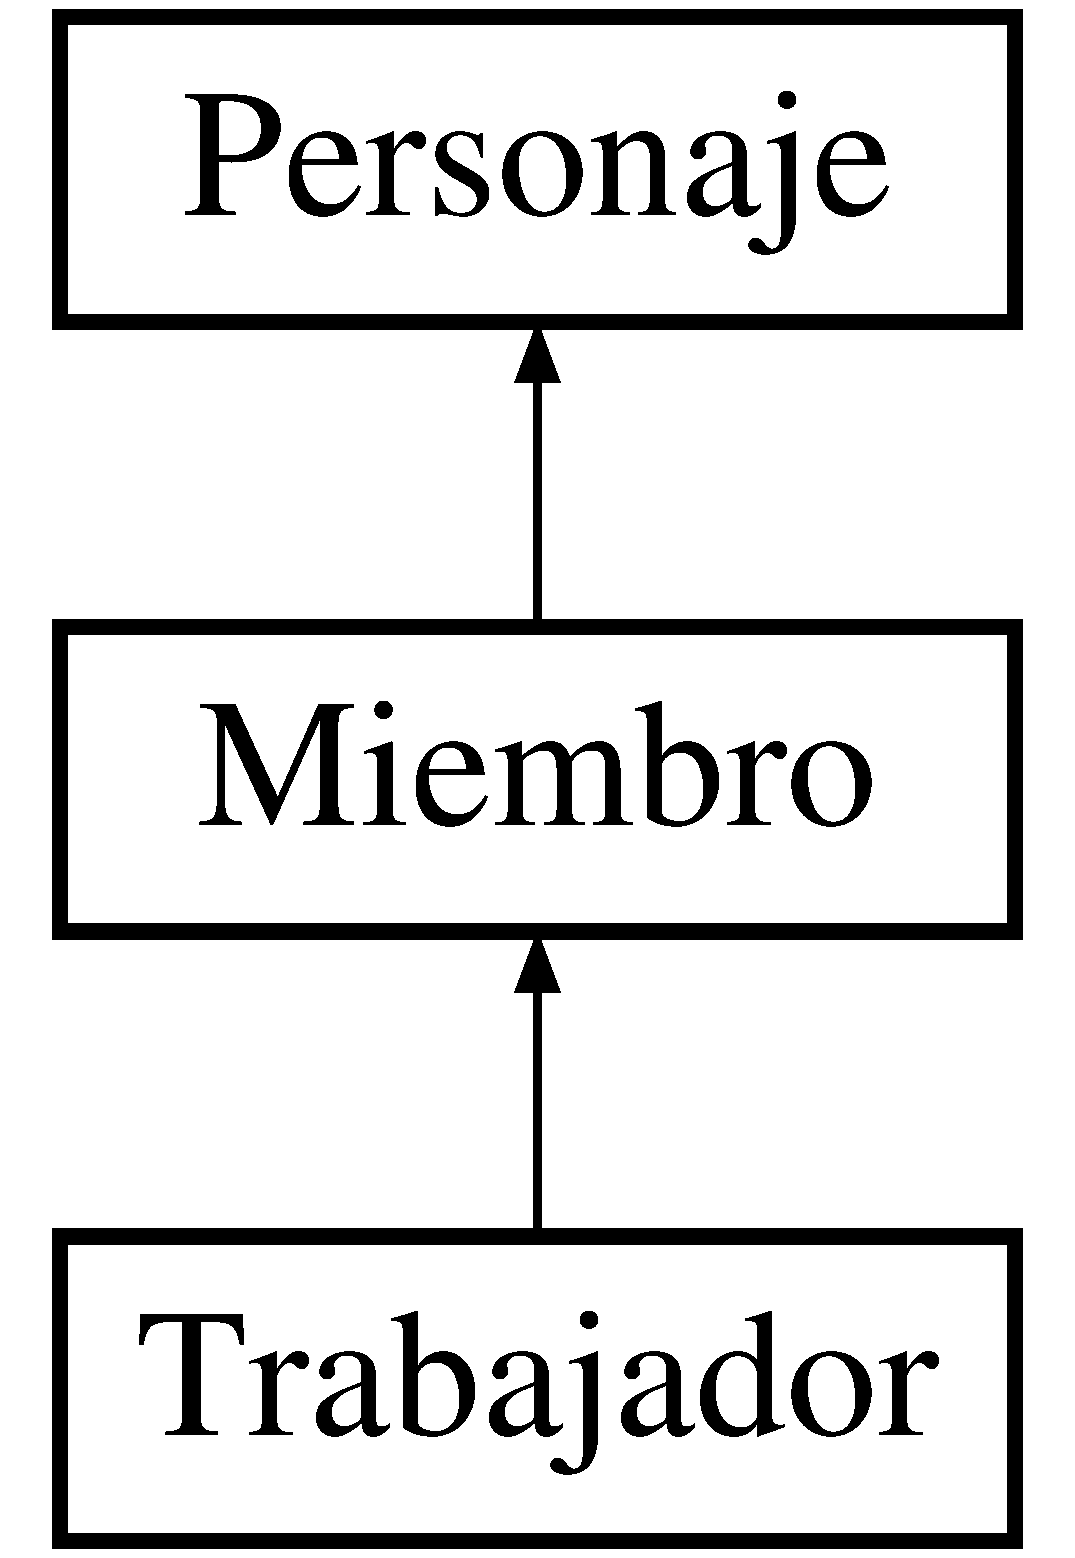
\includegraphics[height=3cm]{classTrabajador}
\end{center}
\end{figure}
\subsection*{Public Member Functions}
\begin{CompactItemize}
\item 
\hyperlink{classTrabajador_3238c3ef60a3e888aa1995399fbee23d}{Trabajador} ()
\item 
\hyperlink{classTrabajador_0596d6d4ac1eaab49ccabb42dfd2fc68}{Trabajador} (char m, string n, int t, int ids, int idp)
\item 
void \hyperlink{classTrabajador_49e5a94181d6a517d9f5213335da1e27}{mostrar} ()
\item 
void \hyperlink{classTrabajador_332796b26094df07fa7b8b39c345f8f4}{escribeLog} (ofstream \&f)
\item 
void \hyperlink{classTrabajador_6b940e57a18466eafa2dcfe0a60313d3}{ruta} (ofstream \&f)
\item 
void \hyperlink{classTrabajador_ae7afce778764088e53c23b21876ac96}{escribeLogRuta} (ofstream \&f)
\item 
void \hyperlink{classTrabajador_ea6e8089295c87f0b5a5014895f28526}{accionUno} ()
\item 
void \hyperlink{classTrabajador_598df69f74628e4da5d0dc776c98b114}{accionDos} ()
\item 
void \hyperlink{classTrabajador_9203576ae93a8854b033f1d91e25fee7}{accionTres} ()
\item 
\hyperlink{classTrabajador_aa31c7df293b6d054e0e41e4b0e27412}{$\sim$Trabajador} ()
\end{CompactItemize}


\subsection{Detailed Description}
\begin{Desc}
\item[Author:]Carlos,,, $<$carlos-linux$>$ \end{Desc}


\subsection{Constructor \& Destructor Documentation}
\hypertarget{classTrabajador_3238c3ef60a3e888aa1995399fbee23d}{
\index{Trabajador@{Trabajador}!Trabajador@{Trabajador}}
\index{Trabajador@{Trabajador}!Trabajador@{Trabajador}}
\subsubsection[Trabajador]{\setlength{\rightskip}{0pt plus 5cm}Trabajador::Trabajador ()}}
\label{classTrabajador_3238c3ef60a3e888aa1995399fbee23d}


Constructor por defecto de mi clase trabajador \begin{Desc}
\item[Parameters:]
\begin{description}
\item[{\em \char`\"{}\char`\"{}}]no recibe parametros \end{description}
\end{Desc}
\begin{Desc}
\item[Returns:]no retorna ningun valor \end{Desc}
\hypertarget{classTrabajador_0596d6d4ac1eaab49ccabb42dfd2fc68}{
\index{Trabajador@{Trabajador}!Trabajador@{Trabajador}}
\index{Trabajador@{Trabajador}!Trabajador@{Trabajador}}
\subsubsection[Trabajador]{\setlength{\rightskip}{0pt plus 5cm}Trabajador::Trabajador (char {\em m}, \/  string {\em n}, \/  int {\em t}, \/  int {\em ids}, \/  int {\em idp})}}
\label{classTrabajador_0596d6d4ac1eaab49ccabb42dfd2fc68}


Constructor parametrizado de mi clase \hyperlink{classTrabajador}{Trabajador} \begin{Desc}
\item[Parameters:]
\begin{description}
\item[{\em m}]es un parametro de entrada del tipo char asociado al atributo marca de mi clase \hyperlink{classPersonaje}{Personaje} \item[{\em n}]es un parametro de entrada del tipo string asociado al atributo Nombre de mi clase \hyperlink{classPersonaje}{Personaje} \item[{\em t}]es un parametro de entrada del tipo entero asociado al atributo turno de mi clase \hyperlink{classPersonaje}{Personaje} \item[{\em ids}]es un parametro de entrada del tipo entero asociado al atributo idsala de mi clase \hyperlink{classPersonaje}{Personaje} \item[{\em idp}]es un parametro de entrada del tipo entero asociado al atributo idplanta de mi clase \hyperlink{classPersonaje}{Personaje} \end{description}
\end{Desc}
\begin{Desc}
\item[Returns:]no retorna ningun valor \end{Desc}
\hypertarget{classTrabajador_aa31c7df293b6d054e0e41e4b0e27412}{
\index{Trabajador@{Trabajador}!$\sim$Trabajador@{$\sim$Trabajador}}
\index{$\sim$Trabajador@{$\sim$Trabajador}!Trabajador@{Trabajador}}
\subsubsection[$\sim$Trabajador]{\setlength{\rightskip}{0pt plus 5cm}Trabajador::$\sim$Trabajador ()}}
\label{classTrabajador_aa31c7df293b6d054e0e41e4b0e27412}


Destructor de mi clase \hyperlink{classTrabajador}{Trabajador} \begin{Desc}
\item[Parameters:]
\begin{description}
\item[{\em \char`\"{}\char`\"{}}]no recibe parametros \end{description}
\end{Desc}
\begin{Desc}
\item[Returns:]no retorna ningun valor \end{Desc}


\subsection{Member Function Documentation}
\hypertarget{classTrabajador_49e5a94181d6a517d9f5213335da1e27}{
\index{Trabajador@{Trabajador}!mostrar@{mostrar}}
\index{mostrar@{mostrar}!Trabajador@{Trabajador}}
\subsubsection[mostrar]{\setlength{\rightskip}{0pt plus 5cm}void Trabajador::mostrar ()\hspace{0.3cm}{\tt  \mbox{[}virtual\mbox{]}}}}
\label{classTrabajador_49e5a94181d6a517d9f5213335da1e27}


Metodo que muestra por pantalla el tipo de personaje del cual se trata, en este caso, trabajador \begin{Desc}
\item[Parameters:]
\begin{description}
\item[{\em \char`\"{}\char`\"{}}]no recibe parametros \end{description}
\end{Desc}
\begin{Desc}
\item[Returns:]no retorna ningun valor \end{Desc}


Reimplemented from \hyperlink{classMiembro_28498c7229e81e64d0cb7ea69515dca0}{Miembro}.\hypertarget{classTrabajador_332796b26094df07fa7b8b39c345f8f4}{
\index{Trabajador@{Trabajador}!escribeLog@{escribeLog}}
\index{escribeLog@{escribeLog}!Trabajador@{Trabajador}}
\subsubsection[escribeLog]{\setlength{\rightskip}{0pt plus 5cm}void Trabajador::escribeLog (ofstream \& {\em f})\hspace{0.3cm}{\tt  \mbox{[}virtual\mbox{]}}}}
\label{classTrabajador_332796b26094df07fa7b8b39c345f8f4}


Metodo que escribe en mi registro.log la informacion correspondiente al trabajador \begin{Desc}
\item[Parameters:]
\begin{description}
\item[{\em f}]es un flujo de entrada salida \end{description}
\end{Desc}
\begin{Desc}
\item[Returns:]no retorna ningun valor \end{Desc}


Reimplemented from \hyperlink{classPersonaje_86fe4a1ff708072d98c6be42bbd512ea}{Personaje}.\hypertarget{classTrabajador_6b940e57a18466eafa2dcfe0a60313d3}{
\index{Trabajador@{Trabajador}!ruta@{ruta}}
\index{ruta@{ruta}!Trabajador@{Trabajador}}
\subsubsection[ruta]{\setlength{\rightskip}{0pt plus 5cm}void Trabajador::ruta (ofstream \& {\em f})\hspace{0.3cm}{\tt  \mbox{[}virtual\mbox{]}}}}
\label{classTrabajador_6b940e57a18466eafa2dcfe0a60313d3}


Metodo que llama al escribelogRuta de mi clase \hyperlink{classTrabajador}{Trabajador} \begin{Desc}
\item[Parameters:]
\begin{description}
\item[{\em f}]es un flujo de entrada salida \end{description}
\end{Desc}
\begin{Desc}
\item[Returns:]no retorna ningun valor \end{Desc}


Reimplemented from \hyperlink{classPersonaje_f6dc20013805229005dfb87fc6f273b5}{Personaje}.\hypertarget{classTrabajador_ae7afce778764088e53c23b21876ac96}{
\index{Trabajador@{Trabajador}!escribeLogRuta@{escribeLogRuta}}
\index{escribeLogRuta@{escribeLogRuta}!Trabajador@{Trabajador}}
\subsubsection[escribeLogRuta]{\setlength{\rightskip}{0pt plus 5cm}void Trabajador::escribeLogRuta (ofstream \& {\em f})}}
\label{classTrabajador_ae7afce778764088e53c23b21876ac96}


Metodo que escribe en mi registro.log la informacion correspondiente a la ruta del trabajador \begin{Desc}
\item[Parameters:]
\begin{description}
\item[{\em f}]es un flujo de entrada salida \end{description}
\end{Desc}
\begin{Desc}
\item[Returns:]no retorna ningun valor \end{Desc}
\hypertarget{classTrabajador_ea6e8089295c87f0b5a5014895f28526}{
\index{Trabajador@{Trabajador}!accionUno@{accionUno}}
\index{accionUno@{accionUno}!Trabajador@{Trabajador}}
\subsubsection[accionUno]{\setlength{\rightskip}{0pt plus 5cm}void Trabajador::accionUno ()\hspace{0.3cm}{\tt  \mbox{[}virtual\mbox{]}}}}
\label{classTrabajador_ea6e8089295c87f0b5a5014895f28526}


Metodo realiza la accion uno correspondiente al trabajador \begin{Desc}
\item[Parameters:]
\begin{description}
\item[{\em \char`\"{}\char`\"{}}]no recibe parametros \end{description}
\end{Desc}
\begin{Desc}
\item[Returns:]no retorna ningun valor \end{Desc}


Reimplemented from \hyperlink{classPersonaje_0454b75ccc8f7e33f03e2cfb2c59e725}{Personaje}.\hypertarget{classTrabajador_598df69f74628e4da5d0dc776c98b114}{
\index{Trabajador@{Trabajador}!accionDos@{accionDos}}
\index{accionDos@{accionDos}!Trabajador@{Trabajador}}
\subsubsection[accionDos]{\setlength{\rightskip}{0pt plus 5cm}void Trabajador::accionDos ()\hspace{0.3cm}{\tt  \mbox{[}virtual\mbox{]}}}}
\label{classTrabajador_598df69f74628e4da5d0dc776c98b114}


Metodo realiza la accion dos correspondiente al trabajador \begin{Desc}
\item[Parameters:]
\begin{description}
\item[{\em \char`\"{}\char`\"{}}]no recibe parametros \end{description}
\end{Desc}
\begin{Desc}
\item[Returns:]no retorna ningun valor \end{Desc}


Reimplemented from \hyperlink{classPersonaje_af7763eb6099390038b7833129a1ef9f}{Personaje}.\hypertarget{classTrabajador_9203576ae93a8854b033f1d91e25fee7}{
\index{Trabajador@{Trabajador}!accionTres@{accionTres}}
\index{accionTres@{accionTres}!Trabajador@{Trabajador}}
\subsubsection[accionTres]{\setlength{\rightskip}{0pt plus 5cm}void Trabajador::accionTres ()\hspace{0.3cm}{\tt  \mbox{[}virtual\mbox{]}}}}
\label{classTrabajador_9203576ae93a8854b033f1d91e25fee7}


Metodo realiza la accion tres correspondiente al trabajador \begin{Desc}
\item[Parameters:]
\begin{description}
\item[{\em \char`\"{}\char`\"{}}]no recibe parametros \end{description}
\end{Desc}
\begin{Desc}
\item[Returns:]no retorna ningun valor \end{Desc}


Reimplemented from \hyperlink{classPersonaje_85c25ff0362bf4f4f5e69965c1ae4cfb}{Personaje}.

The documentation for this class was generated from the following files:\begin{CompactItemize}
\item 
Desktop/academia\_\-lp2/EC3\_\-LPII/src/trabajador.h\item 
Desktop/academia\_\-lp2/EC3\_\-LPII/src/trabajador.cpp\end{CompactItemize}

\chapter{File Documentation}
\hypertarget{arbol_8h}{
\section{Desktop/academia\_\-lp2/EC3\_\-LPII/src/arbol.h File Reference}
\label{arbol_8h}\index{Desktop/academia\_\-lp2/EC3\_\-LPII/src/arbol.h@{Desktop/academia\_\-lp2/EC3\_\-LPII/src/arbol.h}}
}
Declaración de la clase Árbol Binario de Búsqueda. 

{\tt \#include $<$iostream$>$}\par
\subsection*{Classes}
\begin{CompactItemize}
\item 
class \hyperlink{classArbol}{Arbol$<$ T $>$}
\begin{CompactList}\small\item\em Esta clase define un Árbol Binario de Búsqueda. \item\end{CompactList}\item 
class \hyperlink{classArbol_3_01T_01_5_01_4}{Arbol$<$ T $\ast$ $>$}
\begin{CompactList}\small\item\em ÁRBOL GENÉRICO ESPECIALIZADO. \item\end{CompactList}\end{CompactItemize}
\subsection*{Defines}
\begin{CompactItemize}
\item 
\#define \hyperlink{arbol_8h_9eeb8ade5c948220247864bf58da2272}{DEPURAR}~0
\item 
\#define \hyperlink{arbol_8h_4c758869d4ed860db7c6a48f88601c67}{DEPURAR\_\-MSG}(msg)~if (DEPURAR)\{ cout$<$$<$msg; \}
\end{CompactItemize}


\subsection{Detailed Description}
Declaración de la clase Árbol Binario de Búsqueda. 

\begin{Desc}
\item[Author:]{\bf Profesores} LPII \par
 {\bf Asignatura} Laboratorio de Programacion II \par
 {\bf Curso} 07/08 {\bf Revisado} en: Curso 10/11 \end{Desc}


\subsection{Define Documentation}
\hypertarget{arbol_8h_9eeb8ade5c948220247864bf58da2272}{
\index{arbol.h@{arbol.h}!DEPURAR@{DEPURAR}}
\index{DEPURAR@{DEPURAR}!arbol.h@{arbol.h}}
\subsubsection[DEPURAR]{\setlength{\rightskip}{0pt plus 5cm}\#define DEPURAR~0}}
\label{arbol_8h_9eeb8ade5c948220247864bf58da2272}


Variable constante utilizada para mostrar o no mensajes de depuración de programa \hypertarget{arbol_8h_4c758869d4ed860db7c6a48f88601c67}{
\index{arbol.h@{arbol.h}!DEPURAR\_\-MSG@{DEPURAR\_\-MSG}}
\index{DEPURAR\_\-MSG@{DEPURAR\_\-MSG}!arbol.h@{arbol.h}}
\subsubsection[DEPURAR\_\-MSG]{\setlength{\rightskip}{0pt plus 5cm}\#define DEPURAR\_\-MSG(msg)~if (DEPURAR)\{ cout$<$$<$msg; \}}}
\label{arbol_8h_4c758869d4ed860db7c6a48f88601c67}


Macro utilizada paa mostrar mensajes de depuración de programa y retener los mensajes en pantalla 
\hypertarget{cargador_8cpp}{
\section{Desktop/academia\_\-lp2/EC3\_\-LPII/src/cargador.cpp File Reference}
\label{cargador_8cpp}\index{Desktop/academia\_\-lp2/EC3\_\-LPII/src/cargador.cpp@{Desktop/academia\_\-lp2/EC3\_\-LPII/src/cargador.cpp}}
}
Práctica 2007-2008. Implementación de la Clase \hyperlink{classCargador}{Cargador}. 

{\tt \#include \char`\"{}cargador.h\char`\"{}}\par
{\tt \#include \char`\"{}estacion.h\char`\"{}}\par


\subsection{Detailed Description}
Práctica 2007-2008. Implementación de la Clase \hyperlink{classCargador}{Cargador}. 

\begin{Desc}
\item[Author:]{\bf Profesores} LPII \par
 {\bf Asignatura} Laboratorio de Programación II \par
 {\bf Curso} 07/08 -- Revisado en Curso 08/09 \end{Desc}

\hypertarget{cargador_8h}{
\section{Desktop/academia\_\-lp2/EC3\_\-LPII/src/cargador.h File Reference}
\label{cargador_8h}\index{Desktop/academia\_\-lp2/EC3\_\-LPII/src/cargador.h@{Desktop/academia\_\-lp2/EC3\_\-LPII/src/cargador.h}}
}
Práctica 2006-2007. Declaracion de la clase \hyperlink{classCargador}{Cargador}. 

{\tt \#include \char`\"{}fichero.h\char`\"{}}\par
{\tt \#include $<$iostream$>$}\par
{\tt \#include $<$cstring$>$}\par
{\tt \#include $<$cstdlib$>$}\par
{\tt \#include \char`\"{}intruso.h\char`\"{}}\par
{\tt \#include \char`\"{}lider.h\char`\"{}}\par
{\tt \#include \char`\"{}trabajador.h\char`\"{}}\par
\subsection*{Classes}
\begin{CompactItemize}
\item 
class \hyperlink{classCargador}{Cargador}
\begin{CompactList}\small\item\em La misión de esta clase es cargar el sistema con los elementos del fichero de configuración. \item\end{CompactList}\item 
struct \textbf{Cargador::DatoMapeo}
\end{CompactItemize}
\subsection*{Defines}
\begin{CompactItemize}
\item 
\#define \hyperlink{cargador_8h_9eeb8ade5c948220247864bf58da2272}{DEPURAR}~0
\item 
\#define \hyperlink{cargador_8h_4c758869d4ed860db7c6a48f88601c67}{DEPURAR\_\-MSG}(msg)~if (DEPURAR)\{ cout$<$$<$msg;\}
\item 
\hypertarget{cargador_8h_741e5457b26889702f43172b789f32da}{
\#define \textbf{NUMELTOSCONF}~4}
\label{cargador_8h_741e5457b26889702f43172b789f32da}

\end{CompactItemize}


\subsection{Detailed Description}
Práctica 2006-2007. Declaracion de la clase \hyperlink{classCargador}{Cargador}. 

\begin{Desc}
\item[Author:]{\bf Profesores} LPII \par
 {\bf Asignatura} Laboratorio de Programación II \par
 {\bf Curso} 07/08 -- Revisado en Curso 08/09 \end{Desc}


\subsection{Define Documentation}
\hypertarget{cargador_8h_9eeb8ade5c948220247864bf58da2272}{
\index{cargador.h@{cargador.h}!DEPURAR@{DEPURAR}}
\index{DEPURAR@{DEPURAR}!cargador.h@{cargador.h}}
\subsubsection[DEPURAR]{\setlength{\rightskip}{0pt plus 5cm}\#define DEPURAR~0}}
\label{cargador_8h_9eeb8ade5c948220247864bf58da2272}


Variable constante utilizada para mostrar o no mensajes de depuración de programa \hypertarget{cargador_8h_4c758869d4ed860db7c6a48f88601c67}{
\index{cargador.h@{cargador.h}!DEPURAR\_\-MSG@{DEPURAR\_\-MSG}}
\index{DEPURAR\_\-MSG@{DEPURAR\_\-MSG}!cargador.h@{cargador.h}}
\subsubsection[DEPURAR\_\-MSG]{\setlength{\rightskip}{0pt plus 5cm}\#define DEPURAR\_\-MSG(msg)~if (DEPURAR)\{ cout$<$$<$msg;\}}}
\label{cargador_8h_4c758869d4ed860db7c6a48f88601c67}


Macro utilizada para mostrar mensajes de depuración de programa y retener los mensajes en pantalla 
\hypertarget{fichero_8cpp}{
\section{Desktop/academia\_\-lp2/EC3\_\-LPII/src/fichero.cpp File Reference}
\label{fichero_8cpp}\index{Desktop/academia\_\-lp2/EC3\_\-LPII/src/fichero.cpp@{Desktop/academia\_\-lp2/EC3\_\-LPII/src/fichero.cpp}}
}
Implementacion de la clase \hyperlink{classFicheroCarga}{FicheroCarga}. 

{\tt \#include \char`\"{}fichero.h\char`\"{}}\par
{\tt \#include \char`\"{}cargador.h\char`\"{}}\par


\subsection{Detailed Description}
Implementacion de la clase \hyperlink{classFicheroCarga}{FicheroCarga}. 

\begin{Desc}
\item[Author:]{\bf Profesores} LPII \par
 {\bf Asignatura} Laboratorio de Programacion II \par
 {\bf Curso} 07/08 -- Revisado en Curso 08/09 \end{Desc}

\hypertarget{fichero_8h}{
\section{Desktop/academia\_\-lp2/EC3\_\-LPII/src/fichero.h File Reference}
\label{fichero_8h}\index{Desktop/academia\_\-lp2/EC3\_\-LPII/src/fichero.h@{Desktop/academia\_\-lp2/EC3\_\-LPII/src/fichero.h}}
}
Práctica 2007-2008. Declaracion de la clase \hyperlink{classFicheroCarga}{FicheroCarga}. 

{\tt \#include $<$fstream$>$}\par
{\tt \#include $<$iostream$>$}\par
{\tt \#include $<$string$>$}\par
\subsection*{Classes}
\begin{CompactItemize}
\item 
class \hyperlink{classFicheroCarga}{FicheroCarga}
\begin{CompactList}\small\item\em Esta clase carga el sistema con los elementos indicados en el fichero de configuración. \item\end{CompactList}\end{CompactItemize}
\subsection*{Defines}
\begin{CompactItemize}
\item 
\hypertarget{fichero_8h_36e4c5a07c063f5e1dff1855dfedca71}{
\#define \hyperlink{fichero_8h_36e4c5a07c063f5e1dff1855dfedca71}{MAXCAMPOS}~8}
\label{fichero_8h_36e4c5a07c063f5e1dff1855dfedca71}

\begin{CompactList}\small\item\em Constante con el número máximo de campos de una línea del fichero de configuración. \item\end{CompactList}\end{CompactItemize}


\subsection{Detailed Description}
Práctica 2007-2008. Declaracion de la clase \hyperlink{classFicheroCarga}{FicheroCarga}. 

\begin{Desc}
\item[Author:]{\bf Profesores} LPII \par
 {\bf Asignatura} Laboratorio de Programación II \par
 {\bf Curso} 07/08 -- Revisado en Curso 08/09 \end{Desc}

\hypertarget{genaleatorios_8cpp}{
\section{Desktop/academia\_\-lp2/EC3\_\-LPII/src/genaleatorios.cpp File Reference}
\label{genaleatorios_8cpp}\index{Desktop/academia\_\-lp2/EC3\_\-LPII/src/genaleatorios.cpp@{Desktop/academia\_\-lp2/EC3\_\-LPII/src/genaleatorios.cpp}}
}
Implementación de la clase \hyperlink{classGenAleatorios}{GenAleatorios}. 

{\tt \#include \char`\"{}genaleatorios.h\char`\"{}}\par


\subsection{Detailed Description}
Implementación de la clase \hyperlink{classGenAleatorios}{GenAleatorios}. 

\begin{Desc}
\item[Author:]{\bf Profesores} LPII \par
 {\bf Asignatura} Laboratorio de Programacion II \par
 {\bf Curso} 08/09 -- Revisado en Curso 09/10 \end{Desc}

\hypertarget{genaleatorios_8h}{
\section{Desktop/academia\_\-lp2/EC3\_\-LPII/src/genaleatorios.h File Reference}
\label{genaleatorios_8h}\index{Desktop/academia\_\-lp2/EC3\_\-LPII/src/genaleatorios.h@{Desktop/academia\_\-lp2/EC3\_\-LPII/src/genaleatorios.h}}
}
Implementación de la clase \hyperlink{classGenAleatorios}{GenAleatorios}. 

{\tt \#include $<$iostream$>$}\par
{\tt \#include $<$cstdlib$>$}\par
\subsection*{Classes}
\begin{CompactItemize}
\item 
class \hyperlink{classGenAleatorios}{GenAleatorios}
\begin{CompactList}\small\item\em Permite generar números aleatorios dentro de un rango determinado. \item\end{CompactList}\end{CompactItemize}


\subsection{Detailed Description}
Implementación de la clase \hyperlink{classGenAleatorios}{GenAleatorios}. 

\begin{Desc}
\item[Author:]{\bf Profesores} LPII \par
 {\bf Asignatura} Laboratorio de Programacion II \par
 {\bf Curso} 08/09 -- Revisado en Curso 09/10 \end{Desc}

\hypertarget{grafo_8cpp}{
\section{Desktop/academia\_\-lp2/EC3\_\-LPII/src/grafo.cpp File Reference}
\label{grafo_8cpp}\index{Desktop/academia\_\-lp2/EC3\_\-LPII/src/grafo.cpp@{Desktop/academia\_\-lp2/EC3\_\-LPII/src/grafo.cpp}}
}
Implementacion de los metodos de la clase grafo. 

{\tt \#include \char`\"{}grafo.h\char`\"{}}\par


\subsection{Detailed Description}
Implementacion de los metodos de la clase grafo. 

\begin{Desc}
\item[Author:]{\bf Profesores} LPII \par
 {\bf Asignatura} Laboratorio de Programacion II \par
 {\bf Curso} 07/08 (revisado 08/09) \end{Desc}

\hypertarget{grafo_8h}{
\section{Desktop/academia\_\-lp2/EC3\_\-LPII/src/grafo.h File Reference}
\label{grafo_8h}\index{Desktop/academia\_\-lp2/EC3\_\-LPII/src/grafo.h@{Desktop/academia\_\-lp2/EC3\_\-LPII/src/grafo.h}}
}
Declaracion de la clase grafo. 

{\tt \#include $<$iostream$>$}\par
{\tt \#include $<$cstdlib$>$}\par
{\tt \#include $<$queue$>$}\par
{\tt \#include $<$set$>$}\par
\subsection*{Classes}
\begin{CompactItemize}
\item 
struct \textbf{TipoArco}
\item 
class \hyperlink{classGrafo}{Grafo}
\begin{CompactList}\small\item\em Esta clase define un grafo. \item\end{CompactList}\end{CompactItemize}
\subsection*{Defines}
\begin{CompactItemize}
\item 
\hypertarget{grafo_8h_729057a178ee98af9ded64aaabc786be}{
\#define \textbf{MAXVERT}~200}
\label{grafo_8h_729057a178ee98af9ded64aaabc786be}

\item 
\hypertarget{grafo_8h_f076440f216f5a40a11563e489f04932}{
\#define \textbf{INFINITO}~9999}
\label{grafo_8h_f076440f216f5a40a11563e489f04932}

\item 
\hypertarget{grafo_8h_eff54931f8088d31b7efb96f3ec47098}{
\#define \textbf{NO\_\-VALOR}~-1}
\label{grafo_8h_eff54931f8088d31b7efb96f3ec47098}

\item 
\#define \hyperlink{grafo_8h_9eeb8ade5c948220247864bf58da2272}{DEPURAR}~0
\item 
\#define \hyperlink{grafo_8h_4c758869d4ed860db7c6a48f88601c67}{DEPURAR\_\-MSG}(msg)~if (DEPURAR)\{ cout$<$$<$msg; cin.get();\}
\end{CompactItemize}
\subsection*{Typedefs}
\begin{CompactItemize}
\item 
\hypertarget{grafo_8h_6a99a7ad424f10e03cd56b48dc4c695e}{
typedef int \textbf{TipoNodoGrafo}}
\label{grafo_8h_6a99a7ad424f10e03cd56b48dc4c695e}

\item 
\hypertarget{grafo_8h_2e8af4d6cbb1eabfbff65a59a9df8516}{
typedef int \textbf{TipoArcoGrafo}}
\label{grafo_8h_2e8af4d6cbb1eabfbff65a59a9df8516}

\item 
\hypertarget{grafo_8h_bed687de7008e513fbbb6a508534e56b}{
typedef TipoArcoGrafo \textbf{TipoMatrizAdyacencia} \mbox{[}MAXVERT\mbox{]}\mbox{[}MAXVERT\mbox{]}}
\label{grafo_8h_bed687de7008e513fbbb6a508534e56b}

\item 
\hypertarget{grafo_8h_9edce5941c20ba5daf42809231fb1a27}{
typedef TipoNodoGrafo \textbf{TipoVectorNodos} \mbox{[}MAXVERT\mbox{]}}
\label{grafo_8h_9edce5941c20ba5daf42809231fb1a27}

\item 
\hypertarget{grafo_8h_62d8e454f77fac83210e8afb8ed27919}{
typedef set$<$ TipoNodoGrafo $>$ \textbf{TipoCjtoNodos}}
\label{grafo_8h_62d8e454f77fac83210e8afb8ed27919}

\end{CompactItemize}


\subsection{Detailed Description}
Declaracion de la clase grafo. 

\begin{Desc}
\item[Author:]{\bf Profesores} LPII \par
 {\bf Asignatura} Laboratorio de Programacion II \par
 {\bf Curso} 07/08 (revisado 08/09) \end{Desc}


\subsection{Define Documentation}
\hypertarget{grafo_8h_9eeb8ade5c948220247864bf58da2272}{
\index{grafo.h@{grafo.h}!DEPURAR@{DEPURAR}}
\index{DEPURAR@{DEPURAR}!grafo.h@{grafo.h}}
\subsubsection[DEPURAR]{\setlength{\rightskip}{0pt plus 5cm}\#define DEPURAR~0}}
\label{grafo_8h_9eeb8ade5c948220247864bf58da2272}


Variable constante utilizada para mostrar o no mensajes de depuracion de programa \hypertarget{grafo_8h_4c758869d4ed860db7c6a48f88601c67}{
\index{grafo.h@{grafo.h}!DEPURAR\_\-MSG@{DEPURAR\_\-MSG}}
\index{DEPURAR\_\-MSG@{DEPURAR\_\-MSG}!grafo.h@{grafo.h}}
\subsubsection[DEPURAR\_\-MSG]{\setlength{\rightskip}{0pt plus 5cm}\#define DEPURAR\_\-MSG(msg)~if (DEPURAR)\{ cout$<$$<$msg; cin.get();\}}}
\label{grafo_8h_4c758869d4ed860db7c6a48f88601c67}


Macro utilizada para mostrar mensajes de depuracion de programa y retener los mensajes en pantalla 
\printindex
\end{document}
